\documentclass[a4paper,11pt]{book}
\usepackage{graphicx}
\usepackage{epsf}
\usepackage{tocbibind}
\usepackage{amsmath}
\usepackage{amsfonts}
\usepackage{color}
\usepackage{titlesec}
\usepackage{titletoc}
\usepackage{algorithm}
\usepackage{algpseudocode}
\usepackage{tools/fancyhdr}
\usepackage{tools/appendix}
\usepackage{setspace}
\usepackage{subfigure}
\usepackage{enumerate}
\usepackage{makeidx}
\usepackage{hyperref}
%\hypersetup{
%    colorlinks,
%    citecolor=black,
%    filecolor=black,
%    linkcolor=black,
%    urlcolor=black
%}
\addtolength{\textheight}{1cm}
\addtolength{\textwidth}{0.8cm}
\addtolength{\voffset}{0.2cm}
\setlength{\oddsidemargin}{0.9cm}
\setlength{\evensidemargin}{0.5cm}
%Henry's non-sense:
%\setlength{\oddsidemargin}{1.0cm}
%\setlength{\evensidemargin}{-0.47cm}
%\setlength{\parindent}{0cm}
\newcommand{\clearemptydoublepage}{\newpage{\pagestyle{empty}\cleardoublepage}}


\def\x{{\bf x}}
\def\r{{\bf r}}
\def\rp{{\bf r^\prime}}
\def\rpp{{\bf r^{\prime\prime}}}
\def\rppp{{\bf r^{\prime\prime\prime}}}
\def\u{{\bf u}}
\def\p{{\bf p}}
\def\k{{\bf k}}
\def\q{{\bf q}}
\def\G{{\bf G}}
\def\R{{\bf R}}
\def\Rs{{\mathcal{R}}}
\def\Gp{{\bf G^\prime}}
\def\sig{$\Sigma$}
\def\inveps{\varepsilon^{-1}}
\def\eps{\varepsilon}
\def\symm{\left\{\mathcal{S}|\mathbf{v}\right\}}
\def\S{\mathcal{S}}
\def\rt{\tilde{r}}
\def\pt{\tilde{p}}
\def\T{\hat{T}}
\def\bra{\langle}
\def\ket{\rangle}
\def\field{\hat{\psi}}
\def\cfield{\hat{\psi}^{\dagger}}
\def\I{\hat{I}}
\def\w{\omega}
\def\wp{\omega^\prime}
\def\wc{{\omega_{\rm C}}}
\def\e{{\rm e}}
\def\E{\varepsilon}
\def\Y{\mathcal{Y}}
\def\H{\hat{H}}
\def\v{\mathbf{v}}
\def\Gs{\mathcal{G}}
\def\P{\hat{P}_{\rm occ}}
\def\mos{$\textrm{MoS}_{2}$~}
\def\ws{$\textrm{WS}_{2}$}
\def\ck{c_{\k\uparrow}}
\def\ckp{c^{+}_{\k\uparrow}}
\def\cmk{c_{-\k\downarrow}}
\def\cmkp{c^{+}_{-\k\downarrow}}
\definecolor{yellow}{rgb}{1,1,0}
\definecolor{lightblue}{rgb}{0.6,0.6,0.9}
%\sethlcolor{yellow}


\renewcommand{\thechapter}{\arabic{chapter}}
\renewcommand*{\thesection}{\arabic{section}}
\renewcommand{\thesubsection}{\arabic{section}.\arabic{subsection}}
%\setlength{\cftsecnumwidth}{3em}
\titleformat  {\chapter}[hang]{\bfseries\huge\centering}{\thechapter}{2pc}{}{}
\titlespacing {\chapter}{0pt}{0pt}{16pt}{}
\titleformat  {\section}[hang]{\bfseries\large}{\thesection}{2pc}{}{}
\titlespacing {\section}{0pt}{8pt}{6pt}{}
\titleformat  {\subsection}[hang]{\bfseries}{\thesubsection}{2pc}{}{}
\titlespacing {\subsection}{0pt}{10pt}{10pt}{}


\usepackage[sort&compress]{natbib}
\setlength{\bibsep}{0.0pt}
\bibpunct{[}{]}{,}{n}{,}{,}
\makeindex

\begin{document}
\frontmatter
\title{A Material Modeller's Notebook}
\author{Henry Lambert \\
\vspace{0.2cm} 
King's College London \\
\vspace{0.2cm}
{\it with divers and entertaining contributions from}\\
\vspace{0.2cm}
Daniel Corbett\\
\vspace{0.2cm}
University of Manchester
}

\maketitle
\pagenumbering{roman}
\makeatletter
\tableofcontents

\mainmatter
\pagenumbering{arabic}

\chapter{Introduction}
\section{Electronic Structure for Materials Science}
In 1987 Henry Ehrenreich published an article in Science called
``Electronic Theory for Materials Science". The article begins
with what might now be considered a bold statement:

\begin{quote}
Theoretical Materials Science remains to be invented as a discipline, and for good reason.
\end{quote}

The reason he supplies is that materials processing, historically, was a craft. 

It may serve our purposes to consider what exactly constitutes a craft. 
%
There is some sense that the word craft in its common usage 
is to be distinguished from both from science and from art.
%
The word occupies a space somewhere between those two realms. 
%
While a craft bears an element of science
in its application, perhaps the workers possess precision tools or 
established recipes, the process remains fundamentally informed by 
the choices of the craftsman. These choices will always be personal
and in the course of making those choices some aspect of the craftsmen's 
character is conferred to the final product. 

The rise of automation and mechanization means that the conferral
of the craftsman's character to each individual product is 
somewhat diminished.
Though where bespoke solutions are required it is still possible
to turn to the tailors and blacksmiths, carpenters and masons who
have the knowledge and training to render from raw materials
the desired finished product.

In the realm of materials as craft we may take the example of Roman concrete.
%
Roman engineers learned to manufacture concrete from a 
particular mixture of volcanic sands called pozzolana, which
takes its name from Pozzuoli near Napoli. 
%
The pozzolana was mixed with quicklime, an aggregate, and seawater.

The concrete they produced was of striking quality. 
%
The pantheon today remains standing built with the same concrete poured centuries before.
%
This concrete was particularly resistant to degradation in the presence of moisture.
\footnote{For a description of roman concrete and its use at the port at Pouzol see: Mariano Vasi, 
Itineraire Instructif de Rome à Naples, ou, Description Generale des Monumens Anciens et Modernes, 
Rome: [Mariano Vasi]. 1813, de Beer Itb 1815 V.}. 

This concrete was manufactured without any specific knowledge of microstructure and 
chemistry. How the precise mixture even came to be discovered is somewhat mysterious.

Passing from the Romans to the middle ages we may encounter blacksmiths 
who had over the centuries learned to 
The blacksmit learned to manipulate the hardness of swords 
and shields by controlling the alloying of metals and the 
heat in the tempering process. 

Again the theoretical model they worked with 
lacked the modern conception of atomic composition 
and microstructure.

%
The expertise was developed based on part trial and error, 
part common sense, and part notions; or, in a word, craft.
%
In each case the material practitioner's expertise 
was not acquired based on reasoning from first principles.

\subsection{First Principles}

A comprehensive atomic theory describing the way atoms bind, the forces acting on them, 
the way electrons move through the solids, the way light interacts with electrons in solids
and the techniques to solve the equations governing these behaviours, has only 
arisen in the last 100 years. 
%
Over the past 40 years the combination of the theory and access to computers 
means the possibility of constructing accurate models of materials 
systems beginning from the arrangment of the constituent atoms has
progressed. 
%

This philosophy has given rise to the large field of ``first principles" or {\it ab initio} 
\footnote{ab initio (latin): from the beginning.} modelling. 
%
The basic contention of {\it ab initio} modelling is:  

\begin{quote}
Given the atomic numbers of a collection of atoms 
and the arrangement of those atoms in space 
it should be possible to deduce every other 
physical property of the system from that information.
\end{quote}

The philosophy bears a passing resemblance to the classical idea
that so long as the position and momentum of all particles 
is specified with arbitrary accuracy their subsequent 
trajectories could be predicted. The advent of quantum theory
placed limitations on the specification of position and momentum
effectively frustrating the classical picture of a fully determined
trajectory. 

I suspect first principles modelling has yet to 
achieve the level of sophistication
that classical mechanics had by the end 
of the 19$^{\rm th}$ century. Should it  
achieve that level of sophistication we might anticipate 
new discoveries that completely dash 
our hopes of deriving all the physical properties of a system
from the atomic numbers and positions alone.

The extent to which materials science has evolved to the point of being 
a truly 'first principles' theory is one of the themes of these notes. 
%
%Tracking the evolution of theoretical materials science may also allow 
%researchers to identify the avenues of research that are inefficient, 
%that are potentially obscuring knowledge, and convoluting 
%what is already understood. 
%

To chart this evolution we may begin from Ehrenreich's survey of the field from 30 years ago.

Ehrenreich identified four points that either characterized the state 
of the field of theoretical material science at the time or constituted essential principles 
that a satisfactory theory of materials must possess:
%
\begin{enumerate}[i)]
\item Theory must be closely linked to experiment.
\item Ab initio calculations without approximations are virtually impossible 
      except in model systems.
\item Approximations are frequently based on prior experience rather 
      than on theoretical justification.
\item The study of trends in the properties of homologous materials 
      is a crucial ingredient of a credible theoretical framework.
\end{enumerate}
%
These four observations provide a useful framework to analyze the current state of the field.


\subsection{Scales of Materials Modelling}
What are the scales involved in materials modelling?
On what length scale is it important to treat the interactions
using quantum mechanics? What are the time scales? 
What is a typical number of particles?

Chemists arrived at the mol as a convenient unit for describing
quantities of atoms. A mol is on the order of $10^{23}$ atoms. 
That is a lot of atoms. Setting up a single system of 
equations to describe the motion of and mutual 
interactions of this number of particles is not practical.

More realisitically a suitably macroscopic specimen might be considered to be on the 
order of 200 nm$^{3}$ of material. A sample of material of this size is of the 
same order as the wavelength of visible light and could be
resolved with an optical microscope. Assuming an atomic spacing of 2 tenths 
of a nanometer a dynamical simulation of around a billion atoms 
done using quantum mechanics could be considered a quantum mechanical 
simulation of a macroscopic system. 

To give an idea of the time required to perform a well converged quantum simulation 
250 Fe atoms required 4 hours on 96 nodes of the computer with the same 
specifications noted earlier. There are 2000 electrons in the 
simulation which must be allowed
to rearrange themselves so they find their energetic minimum. 
This calculation yields forces on every 
atom that are calculated to an accuracy greater 
than 0.1 eV/A (electron volts per angstrom).
This accuracy is determined by the limitations 
of the theory employed to perform the simulation
rather than numerical limitations.

If computer technology continues developing at the same rate it has
over the previous 30 years than within 60 years, with 
no developements in the numerical techniques, 
quantum mechanical simulations of systems of 
millions of atoms should be feasible within a 
similar amount of computing time. 

If dynamical properties are of interest the atoms motion must be propagated forward. 
If a time step of a femtosecond ($(10^{-15})$s) is taken between evaluations of the 
forces generating a picosecond of data ($(10^{-12})$s) would require about 5 months 
computing time. Another 12 orders of magnitude efficiency would remain to be found to 
simulate the motion of particles on time scales more familiar to
everyday experience.

These considerations are artificial for two important reasons. The first
is I strongly suspect computational power will not continue developing at the rate
seen over the previous 30 years. 

The second is that even if computational resources did continue growing 
at an equivalent rate; simulations of this nature would be of little value.
The objective of {\it ab initio} modeling is to extract meaningful information
about trends and characteristic properties of different classes of materials. 
Massive simulations generate such a quantity of data they may obscure 
reasoning and consume resources without providing insight and general principles.

If, as Ehrenreich suggests, studying trends in homologous materials 
is truly a necessary component of a satisfactory
theory then these simulations would have to be repeated 
over and over again, for every element in a group,
for each compound in a series, etc... The ``one-off" character of 
numerical calculations makes them unsuitable
as the basis for an actual theory of trends in the 
measurable properties of materials.

There is another strange aspect to the properties of materials.
That is that many properties of materials can be described by a scalar, 
like Young's modulus, Poisson ratios, 
or small tensors to describe the elasticity. 
Even some electronic properties can be described 
using a single number like the dielectric constant of a material.
All these properties of systems are made up of many tiny degrees of freedom.
yet at some point all these variables merge 
into macroscopic parameters.
%{this seems like it might require some additivity element similar to in entropy}

The development in computing hardware is in some ways the easy part to chart. 
Clock speed, transistor density, storage, and the proliferation of high 
performance computing clusters with fast interconnects have greatly extended 
the range of problems that can be treated with numerical simulations
simply by providing more horse power.

Along with advances in hardware there have been a number
of methodological developments. These include compiler 
optimization, modern programming languages, 
shared libraries, object orientation, and stable open source 
platforms for code development, testing, and sharing. 

The important theoretical advances, i.e., the physical principles and
mathematical techniques that enable theoretical materials science 
are more difficult to quantify. Difficult to quantify in what exactly 
they are and what they have enabled. In the following sections, 
we describe in some more detail the actual scale 
of the increse in computing power and try to 
identify the major theoretical pillars of materials modelling.

\section{The Rise of the Computer}
\label{sec:riseofcomp}
The second of Ehrenreich's points addresses the state of
{\it ab initio} calculations in 1988 and
the inherent difficulties in performing them.

The intervening thirty years has seen an enormous extension of computing capacity. 
To demonstrate this we may contrast the machines available at the time
he was writing to those that are widely available at the present time of writing (2017). 

In 1987 an example of a state of the art computer would be the Connection Machine.
\footnote{One of the employees at Thinking Machines Corporation,
the company building the connection machine, was Richard Feynman.
For an interesting discussion of the work they
did at Thinking Machines and Feynman's time there see W. Daniel
Hillis' article in Physics Today 42, 2, 78 (1989).}
%There was a strong focus on design at the company. Some of that
%work can be found at Tamiko Thiel's page}%; \url{http://www.tamikothiel.com/theory/cm_txts/di-frames.html}}
The CM-2 was launched in 1987 it was configured with up to 512 MB of RAM and 25 GB of RAID
hard disk space. It had 65K microprocessors (each with 600 bytes of memory). 
%Support for 32 bit floating point operations meant just over 
%2048 processors in practice per machine.

By contrast the HPC machine presently accessible to the author 
is more easily measured in nodes. Each node in a machine has 2x12 core 
Intel Broadwell processors.
Each node has 128 GB RAM and 120 GB static storage. The machine has in total 720 nodes. 
The processors themselves have up to 10 cores with clock speeds (roughly the speed the
processor can execute instructions) on the order of 3 GHz. A clock speed of 12.5 MHz 
would be representative in 1987. 
Each processor, on the modern machine, has abundant cache 
space of 10x 256 KiB L2 Cache, and 25 MiB of L3 cache,
this is to be compared with 600 bytes in the connection machine. 
Nowadays there could be on the order of 3 billion 
transistors in a single microprocessor;
in 1987 that number would be closer to 100,000. 

Listing specifications doesn't necessarily clarify how much more powerful machines have become, 
but it is striking that in terms of speed, storage, and transistor density 
there are 3-5 orders of magnitude improvements in each category. 
The stability and optimization of compilers and the ease of programmability
of the machines has also improved.

It is this constant development of computing capacity that 
has played an important component in enabling {\it ab initio} calculations. 

\section{Computational Craft}
What sort of computations might a theoretical material scientist
wish to compute? One wish list has been provided by Andersen, a materials scientist
may wish to ``compute groundstate properties such as cohesive energies, interatomic forces, 
charge transfer, and magnetic moments, and also excitation spectra described 
by the one-electron Green's function."\cite{anderson75} To obtain these quantities a
number of intermediate calculations must be performed.

The theoretical engines driving progress in numerical simulations of materials systems are
largely based on obtaining descriptions of the electronic eigenstates via mean field theories
like density functional theory or Hartree-Fock. The effective separation
of core and valence electronic interactions, and the various numerical algorithms for 
computing the eigenstates of electrons in material systems, 
and solving the coupled systems of linear equations which arise 
again and again when doing self-consistent electronic structure calculations.

As a guide to which developments are considered important we may
look at the citation metrics. The foundational papers in theoretical materials science
number their citations in the tens of thousands. Table~\ref{tab:foundation} lists some of the papers in the field which, as
their citation count suggests, have enabled subsequent research. These techniques are divided into
three categories, they are either theoretical justification for a calculation scheme, the description of
a technique that allows for more expedient and/or accurate calculations to be performed, 
or parameterizations of the exchange-correlation functional.

\begin{table}
\resizebox{\columnwidth}{!}{%
\begin{tabular}{|p{6cm}|l|p{6cm}|p{4cm}|}
\hline
Paper & Citations & Development & Category\\
\hline
Inhomogeneous Electron Gas \cite{hohenberg64} & 20,527 & Ground state energy of electron gas is universal functional of the density. & Theory \\
Self-Consistent Equations Including Exchange and Correlation Effects & 26,273 & Self-consistent set of equations for varying electron density. & Theory \\
Linear methods in band theory \cite{andersen75}& 4,822 & Describes LAPW and LMTO approach to electronic structure calculations. & Theory/Implementation \\
Norm-Conserving Pseudopotentials \cite{hamann79} & 2,156 & Nodeless eigenfunctions that match atomic eigenvalues.  & Pseudopotentials \\
Soft self-consistent pseudopotentials in a generalized eigenvalue formalism \cite{vanderbilt90} & 11,560 & Effective pseudopotentials for
first row and transition-metal systems.  & Pseudopotentials \\
Projector augmented-wave method \cite{blochl94paw} & 19,194 & Generalizes pseudopotential and LAPW methods; allows reconstruction of wavefunctions at nucleus.  & Pseudopotentials \\
Efficacious Form for Model Pseudopotentials \cite{kleinman82} & 3,709 & Reduces number of integrals which need to be calculated in
pseudopotential calculations. & Pseudopotentials \\
Special points for Brillouin-zone integrations \cite{monkhorst76} & 21,361 & Brillouin zone integration. & Numerical Integration \\
Ground State of the Electron Gas by a Stochastic Method \cite{ceperley80} & 8,855 & Calculation of the exchange-correlation energy of an electron gas. & Exchange Correlation \\
Self-interaction correction to density-functional approximations for many-electron systems \cite{perdew81} & 11,629 & Parameterization of
Ceperley-Alder data on free electron gas. & Exchange Correlation \\
Accurate and simple analytic representation of the electron-gas correlation energy \cite{perdew91} & 12,296 & Parameterization of exchange
correlation functional. & Exchange Correlation \\
Atoms, molecules, solids, and surfaces: Applications of the generalized gradient approximation for exchange and correlation \cite{perdew92}
& 11,418 & Incorporates information from the gradient of the density. & Exchange Correlation \\
New Method for Calculating the One-Particle Green's Function with Application to the Electron-Gas Problem & 2,599 & A calculation scheme for
obtaining progressively more accurate approximations to the one-electron Green's function. \cite{hedin65} & Theory\\
Electron correlation in semiconductors and insulators: Band gaps and quasiparticle energies \cite{hybertsen86} & 1,929 & Extension of
electronic structure calculations to excited states. & Theory/Implementation \\
Unified Approach for Molecular Dynamics and Density-Functional Theory \cite{car85} & 5,940 & Combined molecular dynamics and density
functional theory. & Theory/Implementation \\
High-precision sampling for Brillouin-zone integration in metals \cite{methfessel89} & 2,908 & Brillouin zone integration. & Numerical Integration Technique \\
Improved tetrahedron method for Brillouin-zone integrations \cite{blochl94} &  2,986 & Brillouin zone integration. & Numerical Integration Technique\\
A new mixing of Hartree–Fock and local density‐functional theories \cite{becke93} & 7,143 & Combining Hartree-Fock and DFT. & Exchange Correlation \\
Generalized Gradient Approximation Made Simple \cite{perdew96} & 47,029 & GGA functionals improved.& Exchange Correlation \\
\end{tabular}
}
\caption{Citations are relevant up to Nov. 2017. Citations are according to the journals in which they appear, the actual number of
citations are much higher. These selections have been chosen as representative of the important theoretical and algorithmic developments
which have enabled subsequent research. In some cases there are a number of contemporary papers which
treat the same problems but failed to "catch on", or describe techniques which differ in an incremental way to the works cited here. 
\label{tab:foundation}}
\end{table}

A criticism of Table~\ref{tab:foundation} is biased towards a "plane wave" conception of electronic structure. 
These methods are suitable for crystalline systems with periodicity and can be pushed 
to describe more disordered systems on the order, as discussed in Sec.\ref{sec:riseofcomp}, 
of 1000 atoms. These sorts of techniques are also most favoured by workers studying metallurgical
systems from first principles and materials with potential electronic applications.

To broadly categorize the workers we can say a material scientist 
is interested in crystals, alloys, ceramics, glasses, and, possibly, rubbers and elastomers. They
worry about energy differences on the order of 100 meV. Chemists are interested in molecules, 
tend to use localized basis sets and exploit Monte Carlo and related methods to obtain energy 
bounds on the order of a few meV. Physicists are interested in lasers, Ising and Hubbard models, and the 
general positions of resonances and asymptotes in very cold materials and won't be discussed further. 
%String theorists and cosmologists are charlatans.

\section{Justification by Utility}
The observation that materials processing has evolved in the manner 
of a craft appears to have been imitated in the development of the 
theory of materials science. Much of first principles modelling is reliant on
the realization that certain approximations work well. The first is 
the separatation of degrees of freedom. That is that some electrons in a solid are
tightly bound to a nucleus and behave similarly to how they might behave in an atom.
This allows these "core electrons" to be frozen out of a calculation, via some transformation,
and only valence electrons need to be considered. This is an important realization in
chemistry as well where it has been long recognized that chemical trends are dominated by
the valence electrons of atoms. Accordingly, chemical elements are grouped together in the table 
by their valency. 

\subsection{Core Electrons and Valence Electrons}
Another successful theoretical development is pseudopotentials. Focusing on the valence electrons 
has worked for chemistry.

\subsection{Exchange and Correlation}
The second approximation which works quite well is mean field treatments of 
electron-electron interactions: the treatment of exchange and correlation. 

If we look at the work done based on parameterization of the exchange correlation functional 
we see the number of citations approaches 100,000. Naturally that figure includes significant 
double counting of citing work, on the other hand  we have not included cross citations between journals in many of the 
figures quoted, so with some lucky canceellation the number is probably representative. 

This parameterization is based on what may be considered an abstract question,
``What might happen if we start squeezing electrons into an imaginary box?".
This imaginary box has been pondered for close to a century now. 
The practical utility of these considerations is unreasonable. 
The outcome of these considerations have resulted in a family of 
unremarkable curves that describe some energy relationship between
the density of electrons at a point in space and an energy. 
The practical consequence is this curve enables the
structural, electronic, and vibrational properties of an 
enormous class of materials to be calculated with creditable accuracy.

Just how creditable this approach is returns again to point three. 
The theoretical justifications for the success of the approach are
secondary to the fact that prior experience suggests these techniques work, 
and the rate of their acceptance and adoption seems to have 
tracked their usage in a positive feedback loop. 

If you look through a typical density functional based electronic structure code it is interesting to look at the routine
responsible for calculating the local exchange correlation potential. The input required is the 
electronic density at a point in space \footnote{Beyond the local density
approximation there a range of increasingly complex parameterizations and
approximations to the exchange-correlation functional. For instance some functionals
require the gradient of the density at a point in space.} This 
density is inserted as the sole argument in a subroutine and a single number is returned. The curve
returned has little more structure than that given in Fig.~\ref{fig:ldapz}. 
%
\begin{figure}
\begin{center}
\graphicspath{{./intro/}}% GNUPLOT: LaTeX picture with Postscript
\begingroup
  \makeatletter
  \providecommand\color[2][]{%
    \GenericError{(gnuplot) \space\space\space\@spaces}{%
      Package color not loaded in conjunction with
      terminal option `colourtext'%
    }{See the gnuplot documentation for explanation.%
    }{Either use 'blacktext' in gnuplot or load the package
      color.sty in LaTeX.}%
    \renewcommand\color[2][]{}%
  }%
  \providecommand\includegraphics[2][]{%
    \GenericError{(gnuplot) \space\space\space\@spaces}{%
      Package graphicx or graphics not loaded%
    }{See the gnuplot documentation for explanation.%
    }{The gnuplot epslatex terminal needs graphicx.sty or graphics.sty.}%
    \renewcommand\includegraphics[2][]{}%
  }%
  \providecommand\rotatebox[2]{#2}%
  \@ifundefined{ifGPcolor}{%
    \newif\ifGPcolor
    \GPcolortrue
  }{}%
  \@ifundefined{ifGPblacktext}{%
    \newif\ifGPblacktext
    \GPblacktextfalse
  }{}%
  % define a \g@addto@macro without @ in the name:
  \let\gplgaddtomacro\g@addto@macro
  % define empty templates for all commands taking text:
  \gdef\gplbacktext{}%
  \gdef\gplfronttext{}%
  \makeatother
  \ifGPblacktext
    % no textcolor at all
    \def\colorrgb#1{}%
    \def\colorgray#1{}%
  \else
    % gray or color?
    \ifGPcolor
      \def\colorrgb#1{\color[rgb]{#1}}%
      \def\colorgray#1{\color[gray]{#1}}%
      \expandafter\def\csname LTw\endcsname{\color{white}}%
      \expandafter\def\csname LTb\endcsname{\color{black}}%
      \expandafter\def\csname LTa\endcsname{\color{black}}%
      \expandafter\def\csname LT0\endcsname{\color[rgb]{1,0,0}}%
      \expandafter\def\csname LT1\endcsname{\color[rgb]{0,1,0}}%
      \expandafter\def\csname LT2\endcsname{\color[rgb]{0,0,1}}%
      \expandafter\def\csname LT3\endcsname{\color[rgb]{1,0,1}}%
      \expandafter\def\csname LT4\endcsname{\color[rgb]{0,1,1}}%
      \expandafter\def\csname LT5\endcsname{\color[rgb]{1,1,0}}%
      \expandafter\def\csname LT6\endcsname{\color[rgb]{0,0,0}}%
      \expandafter\def\csname LT7\endcsname{\color[rgb]{1,0.3,0}}%
      \expandafter\def\csname LT8\endcsname{\color[rgb]{0.5,0.5,0.5}}%
    \else
      % gray
      \def\colorrgb#1{\color{black}}%
      \def\colorgray#1{\color[gray]{#1}}%
      \expandafter\def\csname LTw\endcsname{\color{white}}%
      \expandafter\def\csname LTb\endcsname{\color{black}}%
      \expandafter\def\csname LTa\endcsname{\color{black}}%
      \expandafter\def\csname LT0\endcsname{\color{black}}%
      \expandafter\def\csname LT1\endcsname{\color{black}}%
      \expandafter\def\csname LT2\endcsname{\color{black}}%
      \expandafter\def\csname LT3\endcsname{\color{black}}%
      \expandafter\def\csname LT4\endcsname{\color{black}}%
      \expandafter\def\csname LT5\endcsname{\color{black}}%
      \expandafter\def\csname LT6\endcsname{\color{black}}%
      \expandafter\def\csname LT7\endcsname{\color{black}}%
      \expandafter\def\csname LT8\endcsname{\color{black}}%
    \fi
  \fi
    \setlength{\unitlength}{0.0500bp}%
    \ifx\gptboxheight\undefined%
      \newlength{\gptboxheight}%
      \newlength{\gptboxwidth}%
      \newsavebox{\gptboxtext}%
    \fi%
    \setlength{\fboxrule}{0.5pt}%
    \setlength{\fboxsep}{1pt}%
\begin{picture}(5760.00,3960.00)%
    \gplgaddtomacro\gplbacktext{%
      \csname LTb\endcsname%%
      \put(1078,2420){\makebox(0,0)[r]{\strut{}$-0.1$}}%
      \put(1078,2684){\makebox(0,0)[r]{\strut{}$-0.08$}}%
      \put(1078,2948){\makebox(0,0)[r]{\strut{}$-0.06$}}%
      \put(1078,3211){\makebox(0,0)[r]{\strut{}$-0.04$}}%
      \put(1078,3475){\makebox(0,0)[r]{\strut{}$-0.02$}}%
      \put(1078,3739){\makebox(0,0)[r]{\strut{}$0$}}%
      \put(1210,2200){\makebox(0,0){\strut{}$0$}}%
      \put(2041,2200){\makebox(0,0){\strut{}$0.2$}}%
      \put(2871,2200){\makebox(0,0){\strut{}$0.4$}}%
      \put(3702,2200){\makebox(0,0){\strut{}$0.6$}}%
      \put(4532,2200){\makebox(0,0){\strut{}$0.8$}}%
      \put(5363,2200){\makebox(0,0){\strut{}$1$}}%
    }%
    \gplgaddtomacro\gplfronttext{%
      \csname LTb\endcsname%%
      \put(198,3079){\rotatebox{-270}{\makebox(0,0){\strut{}Energy (Ry.)}}}%
      \csname LTb\endcsname%%
      \put(4376,3566){\makebox(0,0)[r]{\strut{}PZ Correlation Energy}}%
    }%
    \gplgaddtomacro\gplbacktext{%
      \csname LTb\endcsname%%
      \put(946,704){\makebox(0,0)[r]{\strut{}$-1$}}%
      \put(946,915){\makebox(0,0)[r]{\strut{}$-0.8$}}%
      \put(946,1126){\makebox(0,0)[r]{\strut{}$-0.6$}}%
      \put(946,1338){\makebox(0,0)[r]{\strut{}$-0.4$}}%
      \put(946,1549){\makebox(0,0)[r]{\strut{}$-0.2$}}%
      \put(946,1760){\makebox(0,0)[r]{\strut{}$0$}}%
      \put(1078,484){\makebox(0,0){\strut{}$0$}}%
      \put(1935,484){\makebox(0,0){\strut{}$0.2$}}%
      \put(2792,484){\makebox(0,0){\strut{}$0.4$}}%
      \put(3649,484){\makebox(0,0){\strut{}$0.6$}}%
      \put(4506,484){\makebox(0,0){\strut{}$0.8$}}%
      \put(5363,484){\makebox(0,0){\strut{}$1$}}%
    }%
    \gplgaddtomacro\gplfronttext{%
      \csname LTb\endcsname%%
      \put(198,1232){\rotatebox{-270}{\makebox(0,0){\strut{}Energy (Ry.)}}}%
      \put(3220,154){\makebox(0,0){\strut{}$\rho$ (e/a.u.$^{3}$)}}%
      \csname LTb\endcsname%%
      \put(4376,1587){\makebox(0,0)[r]{\strut{}PZ Exchange Energy}}%
    }%
    \gplbacktext
    \put(0,0){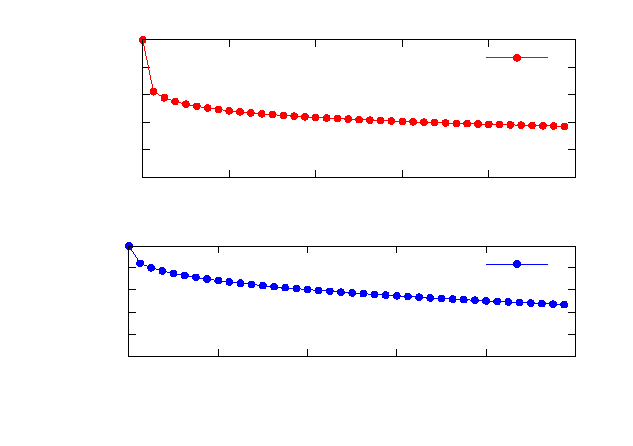
\includegraphics{pz}}%
    \gplfronttext
  \end{picture}%
\endgroup

\caption{Perdew-Zunger parameterization of the correlation and exchange energies for an electron gas.
This curve and those like it enable a great deal of contemporary materials modelling. For reference
a crystal of iron would have an electronic density of around 0.36 e/a.u.$^{3}$ (electrons per cubic
atomic unit). A silicon crystal would have an electronic density in the range of 0.02 e/a.u.$^{3}$,
carbon in the diamond conformation would be around 0.1 e/a.u.$^{-3}$.  
\label{fig:ldapz}.}
\end{center}
\end{figure}
%
Curves of this type have been used to perform calculations and simulations for 
materials composed of elements from across the periodic table. They have been
used to compute all the properties of interest, cohesive energies, magnetic moments,
etc. with varying degrees of success.

Despite its apparent simplicity, in all manner of crystalline systems, 
this functional enables the theoretical
prediction of accurate ground state properties and structures entirely from first principles. 
There are trends at the moment to reparameterize the exchange-correlation functional
in order that simulations return a better description of experimental data. The extent
to which this reparameterization is helpful is debateable. 

Part of the appeal of the simplest local density approximations is that it is universal. 
Where a calculation fails to reproduce an experimental data point, and this failure is attributed to the
exchange correlation functional, it will be argued that applying a more sophisticated treatment
is preferred to introducing a complicated reparameterization of the exchange correlation
function, based on a mixture of theoretical and post hoc experimental justification.

\section{Bayesian Materials Science}
The ubiquity of access to {\it ab initio} data has had a significant impact on 
Ehrenreich's first point: experimental corroboration. 
Cursory surveys of the literature demonstrate the increasing frequency of 
appearance of publications which contain no original experimental work. 

This is partly down to the high level of specialization of contemporary 
researchers and research groups. Previously, the distinction between
an experimental materials scientist and a theoretical one was not so clear cut. 
In addition many important theoretical developments came 
from the context of attempting to explain a new set of experimental data.
%This paragraph needs research:
%Bethe's calculation of the hyperfine? shift, the recursion work on the magnetic 
%moment of $FeAl_{3}$, I think Bardeen mentioned his work on superconductivity was
%initiated when they were trying, Shockley's work on the transistor. (A good source 
%for these sorts of anecdotal history can be found in Nobel prize banquet speeches.)
Ehrenreich's four points help clarify a desirable objective for materials modelling:
a minimal theoretical model informed by {\it ab initio} calculations that accounts for 
experimental data, and {\it predicts quantitatively} trends in material properties. 

In these notes the possibility of exploiting the invariance theorem 
and recursion techniques is assessed as the optimal framework
for achieving this. 

A metric for the quality of the approach can be defined using 
Bayesian probability theory. The Bayesian framework lets us define a metric 
that increases as the number of free parameters in the model is reduced,
and the reproduction of target experimental data is increased, 
with a bound on optimal predictions.

The posterior on the parameters of the model can be assessed:
%
\begin{equation}
\label{eq:bayes}
P(\mathbf{w}|D, \mathcal{H}_{i}) = 
\frac{P(D|\mathbf{w}, \mathcal{H}_{i})P(\mathbf{w}|\mathcal{H})}{P(D|\mathcal{H}_{i})},
\end{equation}
%
where D, the target data, should constitute experimental data. 
Eq.~\ref{eq:bayes} MacKay summarises as:
%
\begin{equation}
{\rm Posterior} = \frac{{\rm Likelihood} \times {\rm Prior}}{{\rm Evidence}}
\end{equation}
%
\begin{equation}
\label{eq:bayesH}
P(\mathcal{H}_{i}|D) \propto P(D|\mathcal{H}_{i})P(\mathcal{H}_{i})
\end{equation}
%
\begin{equation}
\label{eq:bayesH}
P(D|\mathcal{H}_{i}) = P(D|\mathbf{w}, \mathcal{H}_{i})P(\mathbf{w}|\mathcal{H}_{i})d\mathbf{w}
\end{equation}
%
Models (hypotheses) of material systems can then be ranked according to Eq.~\ref{eq:bayesH},  

\section{Prospective}
The purpose of these notes is to establish a framework 
for mapping first principles knowledge about material systems 
onto concise mathematical models. 
%
These models can then be used to compute the properties of materials 
that may be of interest.

The general procedure is to use ab initio data to map 
to well defined local models of the atomic environment. 
The local models of atomic interaction become easier to 
store and manipulate. 

Subsequent chapters will discuss the theory underlying each of these planks; a
theory of the local atomic environment, and the Bayesian techniques to select
models according to a mathematical criterion. 
All of these techniques have been developed by other workers 
over a number of years but collecting 
them into a single place still seems a worthwhile endeavour. 
Of particular interest is providing detailed working of the sometimes 
tedious algebra that underlies important results.

%In chapter \ref{chap:odlr} the passage from discrete atomic models to continuum mechanics
%where collective variables, for instance stress and strain tensors, arise is discussed. 
%Finally, in Chapter \ref{chap:bayes} the criterion for assessing the quality of {\it ab initio} 
%models is discussed which ranks models positively according to their ability to 
%describe target experimental data, and penalizes them for the number of 
%adjustable parameters they require.

Ideally a formalism will be arrived at where engineers informed by the 
structure and composition of a material can consult a simple table of 
coefficients and directly perform the necessary computations, 
perhaps even with pen and paper, to compute within a prescribed
level of accuracy, quantum mechanical properties of their system: e.g. 
band gaps, Young's moduli, hardness, conductivities, cohesive energies, 
reflectivity, superconducting transition temperatures, and so on. A real
alchemist's notebook.

\chapter{The Local Atomic Environment}
\label{chap:invariance}
\section{Introduction}
Vol.~35 of Solid State Physics is dedicated to electronic structure
theory from the point of view of the local environment. This perspective
has a long tradition in physical and chemical electronic structure theory.
This chapter is purely a summary of the work developed there.

Given a Hamiltonian Haydock's Recursion method gives a rapidly convergent 
scheme for computing quantities of interest. The primary quantity of interest 
is the density of states. When this has been computed comparisons between the energetics of 
structures can be made. The method is applicable in situations where Bloch's theorem no longer holds.
A situation which arises at surfaces, in glasses, disordered structures, in structures with a substantial
quantity of impurites, vacancies, defects and dislocations. In short the method is applicable
in realistic physical situations and yields quantities which can be interpreted directly.

%Topics that are often discussed at the beginning of introductory physics courses include:
%the study of black body radiation, photoemission phenomenon, De Broghlie waves,
%electron diffraction experiments and the structure of the hydrogen atom.
%Examination of these topics constitute a suitable foundation 
%for understanding the formalism and experimental justification for the theory.

%It is natural to hope that from the understanding of the electronic states of hydrogen the
%understanding of larger atomic systems, containing progressively more electrons, might emerge. 
%However as the number of electrons in a system grows the wave function becomes 
%somewhat unwieldly to work with and the accurate evaluation of the 
%electron-electron repulsions becomes more difficult. Computers provide a route
%to numerical solutions of the equations governing the behaviour of these systems.
%Computer simulations are commonly performed these days in many branches of physics, 
%chemistry, engineering, and biology. The use of computers to solve Schr\"odinger's 
%equation for electrons in crystals has led to the proliferation of the 
%many, many tribes of electronic structure theory. 
%The tribes are well known to practitioners in the field. A non-exhaustive list
%of some of these we can name here as: tight binding and linear combination of atomic orbitals (LCAO), 
%linear muffing tin orbitals (LMTO), plane waves and pseudopotentials, Gaussian orbitals, and 
%Kohn-Kuttinger-Rostiger theory.
%While successful in a number of respects numerical work can be tedious and, more importantly, can obscure underlying
%mechanisms. There is also a tendency for people working in numerical methods to become 
%excessively obsessed with algorithmic details and, most importantly,
%the results of a single calculation may not provide a framework that accounts for a range
%of phenomenon in homologous series of materials where only slight adjustment of the physical
%interaction parameters change. (This speaks to Ehrenreich third observation 
%that results for homologous materials should be computed
%wherever possible and the results should be compared). 

An example of the economy of explanatory expression afforded by the recursion method
and a physical formulation in terms of the local atomic environment
is Ref.~\cite{johannes76}. In that work 76 crystal structures are correctly predicted 
with a model containing 5 coefficients derived from first principles.

The purpose of this chapter is two fold: firstly to attempt to summarize the incredible range and
detail of theory and application covered in Vol. 35 of Solid State Physics. The secondly
purpose is to speculate on where it should be possible to exploit modern 
computational advantages and the new understanding which has emerged in materials 
to systematically improve descriptions of quantum systems based
on the local environment. 

%

\section{The Invariance Theorem}
\label{sec:invariance}
Heine presents an extended discussion of the invariance
theorem. Heine's section begins, by way of introduction, by pointing 
out an analogy between the the local density of states of a system of interacting
electrons and the black body spectrum of electromagnetic radiation.
Weyl [1911 Math. Ann. 71 441] demonstrated demonstrated the total density
of modes is independent of the shape of the cavity so long as the
radiation is contained in a cavity with dimensions greater than the wavelengths
under consideration. Von Laue [1914 Ann. Phys. Lpz 44 1197] demonstrated that the local density of modes at 
a particular point are exponentially insensitive to the cavity walls.

This analogy has been developed by Friedel [1954 Adv. Phys. 3 446] where
the substition is electromagnetic modes for electronic wavefunctions and
the probability density for finding an electron at a given point
with a given energy replaces the local density of normal modes.\cite{annett94}

The analogy can be seen by writing the density of states,
and the local density of states (for each spin direction) as:
%
\begin{eqnarray}
n(E) = \sum_{n}\delta(E-E_{n}) \\
n(E,\r) = \sum_{n} |\psi_{n}(\r)|^{2}\delta(E-E_{n})
\end{eqnarray}
%
The local density modes of black-body radiation alternatively can be written:
%
\begin{equation}
\rho(\omega,\r)= \sum_{i} |\bra \r| \psi_{i}\ket|^{2}\delta(\omega-\omega_{i}),
\end{equation}
%
with $\psi_{i}$ the eigenfunction (of an electromagnetic wave or a wavefunction) for an eigenvalue $\omega_{i}$.\cite{annett94}
The normal modes of a system can be quite quite sensitive to disturbances but the 
local density of modes, averaged over a small frequency interval, is a stable quantity 
insensitive to disturbances more than a few wavelengths away.

The local density of states is related in turn to the diagonal elements of
the Green's function of a system:
%
\begin{equation}
n(E,\r) = -\frac{1}{\pi}{\rm Im}~G(\r,\r,E)
\end{equation}
%

\section{Matching Green's Functions}
The following treatment has been developed by Heine which in turn follows the 
work of Garcia-Moliner and Rubio, and, Velicky and Bartos, Refs.~\cite{garcia69, velicky71, garcia71},
along with the work of Inglesfield in Refs.~\cite{inglesfield71,inglesfield81}.

An intuitive grasp of the theory of matching Green's functions is a key component of a material
modellers outlook. The theme will be returned to time and again throughout these notes and in
practical applications. Entire subfields of materials science which at first appear distinct 
are in effect just different methods of solving the Schr\"odinger equations in a convenient
basis for one region and matching it at the boundary to a convenient basis 
for a solution in another region. Embedding one potential in another, treating impurities,
the interaction between valence electrons and core electrons bound tight to the nucleus all
involve in one way or another matching Green's functions across a surface.

%The perspective that Heine introduces in Vol. 35 of Solid State Physics 

First a change of variables is perform from $\r$ to $\r''$ in 4.1 
and $\r$ to $\r''$ and $\r'$ to $\r$ in 4.3:
%
\begin{equation}
\label{eq:greentot}
[-\frac{1}{2}\nabla^{2}_{\r''} + V(\r'') - E]G(\r'',\r',E)= -\delta(\r''-\r')
\end{equation}
%
\begin{equation}
\label{eq:greenA}
[-\frac{1}{2}\nabla^{2}_{\r''} + V(\r'') - E]G_{A}(\r,\r'',E)= -\delta(\r''-\r')
\end{equation}

Now multiply Eq.~\ref{eq:greentot} by $G_{A}$ and Eq.
\ref{eq:greenA} by $G$ Then integrate over $\r''$ over region A using
Green's theorem:
%
\begin{equation}
\label{eq:greenthm}
\int\int\int(\phi\nabla^{2}\psi - \psi\nabla^{2}\phi)d^{3}\r 
= \int(\phi\nabla\psi-\psi\nabla\phi)d{\mathbf{S}}
\end{equation}
%
We suppress the energy arguments from here on in assuming them to be contained in G. 

obtained by expressions for $G$ by integrating $\r''$ over region $A$.
%
\begin{equation}
\label{eq:green1a}
G(\r,\r') = G_{A}(\r,\r') + \frac{1}{2} \int d\mathbf{S} 
[\frac{\partial G_{A}(\r,\r_{s})}{\partial n_{S}}G(\r_{S},\r') - G_{A}(\r,\r_{S})\frac{\partial G(\r_{S},\r')}{\partial n_{S}}] [\r, \r' \in A]
\end{equation}

$\frac{\partial}{\partial n_{S}}$ denotes the normal component of grad across
the surface S and $\r_{S}$ is a point on S. (The grad term is a directional component
so the sign can change depending on the orientation.)

And in region B:
%
\begin{equation}
\label{eq:green1b}
G(\r,\r') = G_{B}(\r,\r') - \frac{1}{2} \int d\mathbf{S} 
[\frac{\partial G_{B}(\r,\r_{s})}{\partial n_{S}}G(\r_{S},\r')
- G_{B}(\r,\r_{S})\frac{\partial G(\r_{S},\r')}{\partial n_{S}}] [\r, \r' \in B]
\end{equation}
%

A further property has been used:
%
\begin{equation}
G(\r,\r',E) = G(\r',\r,E),
\end{equation}
%
which is often justified on the ground of a time reversal theorem applying 
to the wave functions in the system.

Finally consideration of the case where $\r'$ and $\r''$ are in different regions is required.

With $\r''$ in B and $\r'$ in A Eq.~\ref{eq:greentot} becomes:
%
\begin{equation}
[-\frac{1}{2}\nabla^{2}_{\r''} + V(\r'') - E]G(\r'',\r') = 0,
\end{equation}
%
the delta function is uniformally zero with those spatial constraints.

The next case restricts $\r$ in B:
%
\begin{equation}
[-\frac{1}{2}\nabla^{2}_{\r''} + V(\r'') - E]G_B(\r,\r'')= \delta(\r-\r''),
\end{equation}
%

A similar cross multiplying trick gives:
%
\begin{equation}
\label{eq:green1c}
G(\r,\r') = -\frac{1}{2} \int dS[\frac{\partial G_{B}(\r, \r_{S}}{\partial n_{S}} G(\r_{S},\r')
- G_{B}(\r, \r_{S})\frac{\partial G(\r_{S},\r')}{\partial n_{S}}] \quad [\r~{\rm in}~B, \r'~{\rm in}~A],
\end{equation}
%
and a similar relation for [$\r$ in A and $\r'$ in B].

Eq.~\ref{green1a} and Eq.~\ref{green1b} give solutions for G but 
aren't very useful until the terms $G(\r_S,\r)$ and 
$\frac{\partial G}{\partial n_{S}}$ are eliminated.

From Eq.~\ref{eq:green1a} we let $\r$ tend to the boundary so $\r = \r_{S}$
%
\begin{equation}
\label{eq:greensys1}
G(\r'',\r') = G_{A}(\r''_{S}, \r') + \frac{1}{2} \int d{S}
[\frac{\partial G_{A}(\r''_{S}, \r_{S})}{\partial n_{S}} G(\r_{S},\r) - 
G_{A}(\r''_{S},\r_{S})\frac{\partial{G(\r_{S}, \r')}}{\partial n_{S}}].
\end{equation}
%

The second relation comes from Eq.\ref{eq:green1c} with 
$\r$ in region B and letting $\r$ tend to $\r^{''}_{S}$.
%
\begin{equation}
\label{eq:greensys2}
G(\r''_{S}, \r') = -\frac{1}{2}\int dS [\frac{\partial G_{B}(\r''_{S}, \r_{S})}{\partial n_{S}}
-G_{B}(\r''_{S},\r_{S})\frac{\partial G(\r_{S},\r')}{\partial n_{S}}]
\end{equation}
%

We now dump the cumbersome indices on the position attributes. These
were necessary to motivate the physical argument for how we have a Green's function
description in one region of space, a Green's function description in another, 
and the joined physical system should be some combination of these two descriptions
which match at the interface. The final step is to write Eq.~\ref{eq:greensys1} 
and Eq.~\ref{eq:greensys2} as matrices:
%
\begin{align}
\label{eq:operator1}
g = g_{A} + \frac{1}{2}\G'_{A}g - \frac{1}{2}\G_{A}g' \\
g = -\frac{1}{2}\G'_{B}g + \frac{1}{2}\G_{B}g' \\
\end{align}
%
\begin{align}
\label{eq:operator2}
g & = & [\G^{-1}_{A}(1-\frac{1}{2}\G'_{A}) + \G^{-1}_{B}(1+\frac{1}{2}\G'_{B})]^{-1} \G^{-1}_{A}g_{A} \\
g' & = & [(1-\frac{1}{2}\G'_{A})^{-1}\G_{A} + (1+\frac{1}{2}\G'_{B})^{-1}]^{-1}(1 - \frac{1}{2}\G'_{A})^{-1}2g_{A}
\end{align}
%
$g$, $g_{A}$, $g'$ are vectors in a space $\{\r_{S}\}$ with components $G(\r_{S},\r')$,
$G_{A}(\r_{S},\r')$, $\partial G(\r_{S},\r')/\partial n_{S}$ with $\r'$ fixed.

$\G_{A}$, $\G'_{A}$ are operators in the space with matrix elements
$G_(A)(\r''_{S}, \r_{S})$, $\partial G_{A}(\r''_{S}, \r_{S})/\partial n_{S}$.

Where the inverse in Eq.~\ref{eq:operator1, eq:operator2} 
doesn't exist there is a pole. This is the condition for a discrete energy level 
of the Schrodinger equation for the combined A + B systems. 

Equations written in the form of \ref{eq:green1a} are of the type required for the invariance theorem namely:
%
\begin{equation}
G(\r,\r';E) = G_{A}(\r,\r';E) + {\rm boundary ~ corrections},
\end{equation}
%
where we have restored the energy argument.
These considerations provide a reasonable mathematical framework for 
investigating electronic structure from the point of view of the local environment.
Indeed as Heine himself says: 

\begin{quote}
The importance of this approach would lie in the fact that
one has a single entity $G_{A}$ to represent an element in anything 
from a small molecule to a complex alloy.
\end{quote}

As a practical example the success of planewave and pseudopotential methods 
is reliant on finding decent approximations to the quantity $G_{A}$. The plane waves
in the interstitial regions must match the Green's function for the atomic system
at a particular radial cutoff and energy. If a function can be found that 
describes the scattering of these waves across a suitable energy range the approximation 
is a good one and the matching of the two systems will be successful. This
is represented schematically in Fig.~\ref{fig:pseudosplit}.
%
\begin{figure}
\begin{center}
\includegraphics{./invariance/pseudosplit.png}
\caption{Schematic representation of decomposing the Green's function into a local atom centered
Green's function, $G_{A}$, and the Green's function in the interstitial region $G_{B}$.
A pseudopotential is a function that allows $G_{B}$ to be represented as a relatively
smooth function of position capable of efficient description in terms of plane waves.
The functions must match at the cutoff for $G_{A}$ to the solutions for 
atomic wave functions. Another approach would involve matching the $G_{A}$ 
and $G_{B}$ explicitly at each stage of the calculation until self-consistency is obtained.}
\end{center}
\end{figure}
%
Heine's ambition turns on this:
%
\begin{quote}
We see now that the trick in the new formulation of quantum 
mechanics is not just to express measurable quantities in terms of 
G, {\it but in terms of some appropriate small parts of G that can be solved 
for and computed separately from all the unwanted remainder of G.}
\end{quote}
%
This relies, again in analogy with black bodies, on the Green's
function in a certain region of space being independent of the size and shape
of the container and the boundary conditions.

\section{Slater-Koster Tight Binding}
  Let us denote the translation operator $\hat{T}$
as the operator which displaces all the coordinates of a vector 
by a crystal lattice vector $\R_{i}$ we require 
firstly that $[\hat{T},\hat{H}]=0$, i.e. that the 
translation operator commutes with the Hamiltonian. This also
has the consequence that the eigenvectors of the Hamiltonian
must be eigenvectors of the translation operator. 

Bloch's theorem encapsulates this idea. When a translation operator acts 
on a Bloch state of a crystal the wavefunction is multiplied by a scalar
value $e^{i\k\cdot\R}$: i.e. the condition for a vector to be an
eigenvector.

If a basis set of atomic orbitals $\phi_{n}(\r-\R_{i})$
is placed on each atom in the crystal an un-normalized Bloch sum can be 
written as $\sum_{\R_{i}} e^{i\k\cdot\R_{i}}\phi_{n}(\r-\R_{i})$. For
a given $\k$ there will be off-diagonal elements between Bloch sums
for different atomic orbitals.


The matrix elements between Bloch sums (where L\"owdin orbitals $\psi_{n}$ 
are used instead of LCAOs, \cite{lowdin62}) gives:
%
\begin{equation}
\sum_{\R_{j}} e^{i\k\cdot(\R_{j}-\R_{i})}\times\int \psi^{*}_{n}(\r-\R_{i})H\psi_{m}(\r-\R_{j})dV
\end{equation}
%
The development of computers means the secular equations can be solved 
at arbitrary $\k$ points. \footnote{The paper explicitly anticipates that the integrals and Bloch 
sums could be performed with the help of computers: ``The possibility is not excluded 
that eventually ways will be found to do this work by means of high-speed computers, but
it will certainly be quite out of the question without such help."} 

The work of Slater-Koster demonstrates, in an intuitive fashion, how localized atomic
states, when modulated by a wave of the form $e^{i\k\cdot\R}$ can interfere 
(constructively or deconstructively) to allow charge to accumulate in different 
spatial patterns between atoms, and how the variation in the eigenvalues of $H_{\k}$
can give rise to band structures. Determining the coefficients involved in the 
tight binding energy integrals is somewhat involved. The Coordinate system needs
to be set up and the integrals performed for different combinations of spherical
harmonics on neighbouring atoms. Ref.~\cite{sharma79,podolsky04} both give explicit
expression for generating the coefficients programmatically.

The determination of the integration constants is a problem unto itself.
Tight binding parameters for the transition metals can be extracted from 
a number of places: tight binding parameters that span the transition
metal range can be found in Refs. \cite{nieminen76}, \cite{pettifor77} and \cite{jepsen75, andersen77, harrison80}.
Harrison has also published a set of universal parameters for s-p bonded structures.

\section{Transition Metal Tight Binding}
\label{sec:tmtb}
Bullet discusses some of the problems with treating d electrons in a tight binding 
formalism (Sec. IV 13 Solid State Physics Vol. 35). Fig.~\ref{fig:datoms} demonstrates
one of the main issues arising with d electrons:
%
\begin{figure}
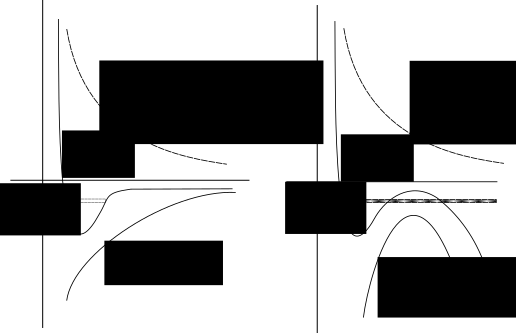
\includegraphics{./invariance/resonant-datoms.pdf}
\caption{The possibility of free electron states, in the interstitial region, 
resonating with atom centered localized states. The centrifugal components of the 
atomic d wave scattering channel can combine with
the atomic potential to produce a bound electronic state at some energy $E^{0}_{l}$ for an atomic system.
In a crystal the atomic periodic potential can be such that electrons can be bound in an
atomic d-like state can have the same energy as tunnel through the barrier localizing 
them and mix with free electron plane wave states. This dual character of the wave 
function, with localized components and extended components, requires careful 
detangling to return to a tight binding description. This difficulty 
stems from the presence of an energy resonance 
complicating the process of choosing the coefficients of the tight binding matrix. 
For the optimal, energy independent, set of coefficients that can be 
chosen see the work of Pettifor. There is a close parallel with the resonant
scattering of d-wave electrons in materials and Feshbach resonances Ref.~\cite{chin10}.
[Figure Taken from D.W. Bullet Solid State Physics Vol. 35 pg. 197.]}
\end{figure}
%

From pseudopotentials we are familiar with having to match the logarithmic energy
derivative at some cutoff radius. Usually found by integrating the radial
Schr\"odinger equation to find $u_{l}(r,\epsilon)$ and matching the logarithmic derivatives:
%
\begin{equation}
L_{l}(\epsilon) \equiv \frac{u'_{l}(r_{0},\epsilon)}{u_{l}(r_{0},\epsilon)} = \frac{\kappa[j'_{l}
(\kappa r_{0}) - \tan \eta_{l} n'_{l}(\kappa r_{0})]} {j_{l}(\kappa r_{0}) - \tan \eta_{l} n_{l}'(\kappa r_{0})]},
\end{equation}
%
where
%
\begin{equation}
\label{eq:phaseshift}
\tan \eta_{l} = \frac{\kappa j'_{l} - L_{l}j_{l}}{\kappa n'_{l} - L_{l}n_{l}}.
\end{equation}

In terms of the energy and width the l=2 phase shift Eq.~\ref{eq:phaseshift} 
can be written:
%
\begin{equation}
\label{eq:dshift}
\tan \eta_{d} = \frac{\frac{1}{2}W(\epsilon)}{\epsilon_{d}-\epsilon}.
\end{equation}
%
The uncertainty principle allows for the estimation of the rest
time for an electron on an atomic d state to be around $\hbar/W_{d}\approx 10^{-14}$s \cite{friedel73}.
\footnote{Ref.~\cite{friedel73}, written in 1973, provides us with another example
of the early impact electronic computers were making in the field. Friedel  compares 
the relative merits of `muffin tin' type calculations and tight binding approximations.
The former approach he describes as leading, ``to fairly exact if cumbersome
computations, and has thus had the support of the `computers lobby'". The conclusion
puts forward a number of points in favour of tight binding approaches as 
being suitable for studying complex phases and lattice defects,
latent heats of phase changes, elastic constants and electron-phonon couplings.}

The strong centrifugal contribution to the
atomic scattering potential from higher angular moment channels means the effective potential
can create a bound atomic state. In a solid the energy of this bound state can match the 
energy of a free electron state in the interstitial region and there will
be resonant tunneling between the two states. This results in the hybridization of d states
and plane waves. 

This means an appropriate model Hamiltonian must account for the various states as
%
\begin{eqnarray}
\label{eq:d-hamiltonian}
H =  d-d  &  d-PW \\
     PW-D & PW-PW 
\end{eqnarray}
%
where d-d and PW-PW are of the tight-binding and plane-wave 
pseudopotential form and hybridization occurring in the 
off-diagonal elements. The dual characteristic of transition metals
tightly bound d-electrons and diffuse s-p orbitals hybridizing 
accounts for the difficulties in describing their electronic properties.


The $dd\sigma$ terms behave roughly as \cite{pettifor71}:
%
\begin{equation}
\label{eq:pettifor}
dd\sigma \approx \frac{-5W\cos\kappa_{d}R}{\kappa_{d}R}
\end{equation}
%
If we write our basis functions in terms of localized orbitals
Eq.~\ref{eq:pettifor} suggests our Hamiltonian matrix will be 
populated by a huge number of off-diagonal matrix elements which can't be neglected. If 
the energy is equal to $k^{2}$ constructive interference occurs and the energy summation
diverges with off-diagonal matrix elements between all d states on remote atoms becoming
significant. This isn't entirely surprising. We are considering a periodic crystalline solid
and the eigenfunctions of this crystal are extended throughout. The off-diagonal elements
in a coordinate space representation reflect the long range order of the material and
preservation of the phase of the electronic wave function as they move from atom to atom. See
Chapter~\ref{chap:odlro} for further discussion of this and related points.

The `best' approximations to the explicit formulas for $dd\sigma$, $dd\pi$ and $dd\delta$ and the phase
shift $d_{0}'$ of the diagonal tight-binding elements 
These difficulty have been addressed in a number of works 
\cite{hubbard67}, \cite{hubbard68}, \cite{hubbard69} \footnote{Another computational
snapshot comes from Ref.~\cite{hubbard69}, "...smaller secular 
equations are used, taking about one second per k point on an IBM  360/65." The
main storage capacity of those machines was 524 kilobytes. See Fig.~\ref{fig:ibm360}
for a (grainy) snapshot of what that computer looked like.},
and J. Hubbard, ibid 2, 1222 (1969). The problem being to define an
energy independent Hamiltonian, amenable to tight binding for the d electrons.

Deriving an effective, tight binding, energy indepedent parameterization
of d electron structure  culminated in the work of D. G. Pettifor's \cite{pettifor69}. 
Pettifor's work produced a justifiable scheme for computing the two center tight binding integrals of Slater
and Koster, $dd\sigma$, $dd\pi$, $dd\delta$ in terms of the position and halfwidth of the resonance:
$\epsilon_0$ and $\Gamma$. It is worthwhile considering the achievement of these collected papers.
With relatively limited computing power the workers determined 
the positions of atomic eigenvalues, band widths, and the effect 
of atomic scattering potentials. In 
the course of the work a great deal of algebraic manipulation of spherical 
harmonics and plane waves is required, along with the determination
of numerical values via graphical methods. All in all a laborious but fruitful task resulting
in energy independent matrix elements localized to nearest (next nearest ) 
neighbours real and reciprocal space.

The work of Pettifor and colleagues in determining justifiable tight 
binding parameters for transitional metals, 
effectively completed by 1969, was an important prerequisite for the subsequent 
development of the recursion method in the 1970s. Generalized tables for tightbinding parameters 
across the transition metal series has been produced in Ref.~\cite{harrison80}.

%The parameters used in Ref.~\cite{burke78} are appropriate to the BCC structure.
%The tightbinding Hamiltonian only considers two center contributions, with the parameters 
%coming from Pettifor\cite{pettifor69} and rescaled to produce the observed
%bandwidth of tungsten. The parameters are given in Table~\ref{tab:dsurface}.

For ease of reference we collect here d tight-binding coefficicents
that have found there way into the literature. The choice of these parameters
is very much an example of theoretical materials science constituting a 
craft. In later chapters we will examine some of the developments that set
tight-binding and the choice of coefficients on a more definite 
theoretical framework. The Slater-Koster parameters used for FCC, BCC, 
and HCP crystals in Ref.~\cite{haydock72} are given in Table \ref{tab:pettiparams}.
%
\begin{table}
\begin{center}
\begin{tabular}{|c|c|c|c|c|} 
\hline
Structure & $dd\sigma$ & $dd\pi$  & $dd\delta$ &  Band-limits \\
\hline
FCC       & -0.027784  & 0.012535 & -0.001554  & -0.131 to 0.085 \\ 
\hline
HCP       & -0.027784  & 0.012535 & -0.001554  & -0.119 to 0.081 \\
\hline
BCC       & -0.03248   & 0.01538  & -0.00200   & -0.119 to 0.097 \\
          & -0.01341   & 0.00487  & -0.00049   &              \\
\hline
\end{tabular}
\caption{Slater-Koster parameters from Pettifor \cite{pettifor69}, 
along with band edges in Ry. First and second nearest neighbour 
parameters are given for BCC crystals. \label{tab:pettiparams}.}
\end{center}
\end{table}
%
%\begin{table}
%\begin{tabular}{|c|c|c|}
%\hline
%SK Parameter & First Neighbour & Second Nearest Neighbour \\
%\hline
%$dd\sigma$ & -0.02992  & -0.05364 \\
%$dd\pi$    &  0.06652  &  0.01943 \\
%$dd\delta$ &  0.00800  &  0.00196 \\
%\hline
%\end{tabular}
%\caption{These parameters are difficult to make out from the electronic version of Ref.
%due to poor resolution of the scan. \label{tab:dsurface}.}
%\end{table}
%
\begin{table}
\begin{center}
\begin{tabular}{|c|c|c|}
\hline
\multicolumn{3}{|c|} {FCC TB Parameters} \\
\hline
Integral & 1st Nearest Neighbour & 2nd Nearest Neighbours \\
\hline
$dd\sigma$ & -0.027784 & - \\
$dd\pi$    &  0.012535 & - \\
$dd\delta$ & -0.001554 & - \\
\hline
\multicolumn{3}{|c|} {BCC TB Parameters} \\
\hline
Integral & 1st Nearest Neighbour & 2nd Nearest Neighbours \\
$dd\sigma$ & -0.06560  & -0.03195 \\
$dd\pi$    &  0.04373  & 0.02130\\
$dd\delta$ & -0.010934 & -0.00537\\
\hline
\end{tabular}
\caption{The tight binding parameters used for the example recursion 
calculations in this chapter, in the FCC lattice only nearest neighbours 
are included.}
\end{center}
\end{table}

Whether we are able to create a tight binding description of transition metals
depends on whether a decent, energy independent, approximation to the electronic 
structure in fcc/bcc metals can be achieved with 9x9 matrices describing 
nearest neighbour interactions of the s, p and d states, in the Slater-Koster 
form or derived from electronic states localized according to some 

\subsection{Kelly Tight Binding}

An example from Kelly helps to make the application of the tightbinding scheme clear:
%
\begin{quote}
As input data we require a convenient local representation of $H$. In simple crystals,
this is most easily given in terms of interactions with a unit cell and between neighboring cells.
For a FCC transition metal we have nine orbitals (1 s-orbital, 3 p-orbitals, and 5 d-orbitals) per site, 
and a diagonal 9x9 matrix for the self-energies of these orbitals. Twelve 9x9 matrices 
suffice to describe the interaction of any atom with its nearest neighbours.
\end{quote}
%

The actual operation of $H|u_{n}\ket$,which has been discussed in a general way so far, 
can be written as:
%
\begin{equation}
H|u_{n}\ket = \sum_{\alpha l \beta j}a_{n \alpha l}(\bra \beta j |H| \alpha l\ket)|\beta j\ket,
\end{equation}
%
to exploit the sparsity of H we introduce an index $z$ which runs over the neighbors of 
site l with which the orbitals interact:
\begin{equation}
H|u_{n}\ket = \sum_{\alpha l z}a_{n \alpha l}(\bra \beta_{z} j_{z} |H^{z}|\alpha l\ket)|\beta_{z} j_{z}\ket.
\end{equation}
There are no restrictions on the number of orbitals per site, or on the range of interactions that can be
incorporated, these only impact on the efficiency of the method and the validity of the original assumptions
about the dominance of the local atomic environment.


\section{Recursion Method}
The principle of the recursion method is to obtain a convergent expression 
for an element of the Green's function:
%
\begin{equation}
G_{\chi\chi}(E) = \bra\chi|[E + i\delta -H]^{-1}|\chi\ket.
\end{equation}
%

The Green's function can be immediately related to the local density of states as:
%
\begin{equation}
n_{\alpha l}(E) = -\frac{1}{\pi} {\rm Im}\bra\alpha l|[E + i\delta -H]^{-1}|\alpha l\ket
\end{equation}
%

The state $\chi$ which we project on to can be made up of some linear combination 
of the local basis set $\phi_{\alpha l}$, which, in turn, could be local atom centered orbitals, bond orbitals, 
Wannier functions, atomic diplacements, or any localized quantity we wish to define. The method is thus
applicable to a wide range of problems in condensed matter. In short what we wish to examine
is determined by the choice of $\chi$.

\subsection{Mathematical Origin}
The trick of the recursion method, if you like to think of things in terms of tricks, 
or its generating feature, if you prefer, is that from the outset the `Greenian', the element
of the Green's function we are interested in, is restricted to a particular matrix element: 
%
\begin{equation}
\label{eq:greenian}
G_{00}(E) = \bra u_{0}|[E-H]^{-1}|u_{0}\ket 
\end{equation}
%
As Heine puts it in his chapter:
%
\begin{quote}
Note that we do not want the whole of the inverse matrix $[E-H]^{-1}$, 
\emph{only one element}, and on this the whole method depends. In physics we do not
usually inquire about the whole of life, but about one particular matrix element (at a time) and we have chosen
$u_{0}$ so that Eq.~\ref{eq:greenian} gives us what, to put it crudely, we want.
\end{quote}

If we are given a tridiagonal matrix of the form:
%
\begin{equation}
H = \begin{bmatrix}
a_0 & b_1 & 0 & 0 & 0 &  ...\\
b_1 & a_1 & b_2 & 0 & 0 &  ...\\
0 & b_2 & a_2 & b_3 & 0 &  ...\\
0 & 0 & b_3 & a_3 & b_4 & ...\\
0 & 0 & 0 & b_4 & a_4 & ...  \\
0 & 0 & 0 & 0 & b_5 & ... 
\end{bmatrix}
\end{equation}

%
The determinants and sub-determinants etc. of the matrix can be nested:
%
$$
\newcommand*{\temp}{\multicolumn{1}{|c|}{b_1}}
\newcommand*{\tempa}{\multicolumn{1}{|c|}{b_2}}
\newcommand*{\tempb}{\multicolumn{1}{|c|}{b_3}}
\newcommand*{\tempc}{\multicolumn{1}{|c}{0}}
\begin{array}{|ccccccc}
\cline{0-5}
a_0 & b_1 & 0 & 0 & 0 & 0  & D_0 \\ \cline{2-6} 
\temp & a_1 & b_2 & 0 & 0 & 0 & D_1 \\ \cline{3-6} 
0 & \tempa & a_2 & b_3 & 0 & 0 & D_2 \\ \cline{4-6}
0 & \tempc &  \tempb &  a_3 & b_4 & ... & D_3
\end{array}
$$

Eq.~\ref{eq:greenian} can be rewritten in terms of its determinants:
%
\begin{equation}
\label{eq:greendet}
\bra u_{0}|[E-H]^{-1}|u_{0}\ket = \frac{{\rm det}|D_{1}|}{{\rm det}|D_{0}|},
\end{equation}
%
or, equivalently, be written as:
%
\begin{equation}
\label{eq:greendet}
\bra u_{0}|[E-H]^{-1}|u_{0}\ket = \frac{1}{\frac{{\rm det}|D_{0}|}{{\rm det}|D_{1}|}}.
\end{equation}
%
Appeal is then made to \index{Cauchy}\footnote{Baron Augustin-Louis Cauchy FRS FRSE (21 August 1789 – 23 May 1857)} 
for the following expansion:
%
\begin{equation}
\label{eq:cauchy}
{\rm det}|D_{0}| = (E-a_{0}){\rm det}|D_{1}|-b^{2}_{1}{\rm det}|D_{2}|
\end{equation}
%
and when generalized to determinants for $|D_{n}|$, $|D_{n+1}|$, and $|D_{n+2}|$:
%
\begin{equation}
\frac{{\rm det}|D_{n}|}{{\rm det}|D_{n+1}|} = E-a_{n}-\frac{b^{2}_{n+1}}{\frac{{\rm det}|D_{n+1}|}{{\rm det}|D_{n+2}|}}
\end{equation}

\footnote{
\index{C. Lanczos} J. Res. Natl. Bur. Stand. 45, 255 (1950) 
used the chain model in numerical work as a way of diagonalizing matrices
that could be implemented efficiently in a computer.
Chebyshev used chain models for approximating functions on an interval
P. L. Chebyshev, Bull. Acad. Imp. Sci. St. Petersbourg 1, 193 (1859)}

The coefficients of the continued fraction can be obtained from
a three term recurrence relation:
%
\begin{equation}
b_{n+1}|u_{n+1}\ket = H |u_{n}\ket - a_{n}|u_{n}\ket - b_{n}|u_{n-1}\ket
\end{equation}

where:
\begin{equation}
a_{n} = \bra u_{n}|H|u_{n} \ket,
\end{equation}
and 
\begin{equation}
b_{n} = \bra u_{n}|H|u_{n-1} \ket.
\end{equation}

\section{Analytic Recursion}
\subsection{The Constant Chain}
The simplest chain model that can be handled analytically is the constant chain and it
serves as the paradigm of all the recursion calculations that will be undertaken. 
The constant chain corresponds to the general continued fraction written:
%
\begin{equation}
\label{eq:constantchain}
G_{0}(E) = \cfrac{1}{E-a_{0}-\cfrac{b_{1}^2}{E-a_{1}-\cfrac{b_{2}^{2}}{E-a_{2}-\cfrac{b_{3}^{2}}{...}}}},
\end{equation}
%
where $a_{0}=a_{1}=...=a_{n}=a$ and $b_{0}=b_{1}=...=b_{n}=b$. 
%
In this chain an electron experiences the same pull to 
every site on the chain, and can hop from one site to 
the next with the same hopping amplitude $b^{2}_{n}$. 
%
That all the coefficients are the same means a closed 
form solution can easily be found by recognizing that 
Eq.~\ref{eq:constantchain} can be written as:
%
\begin{equation}
G_{0}(E) = \frac{1}{E-a-b^{2}G_{0}(E)},
\end{equation}
%
and rearranged to give:
%
\begin{equation}
G_{0}(E) = (\frac{E-a}{2b^{2}}) \pm \sqrt{\frac{1}{4}(\frac{E-a}{b^{2}})^{2} - \frac{1}{b^{2}}}.
\end{equation}

The argument of the Green's function is $E + i\delta$, for positive 
energies the negative root is chosen and for negative energies 
the positive root is chosen. This gives the real
and imaginary part of the Green's function plotted 
in Fig.~\ref{fig:gfconstchain}.
%
\begin{figure}
\begin{center}
{\graphicspath{{./invariance/chain_figs/}}\input{./invariance/chain_figs/chain_plot.tex}}
\caption{Real and imaginary parts of the Green's function for the constant chain.\label{fig:gfconstchain}}
\end{center}
\end{figure}
%
The constant chain yields an analytic solution. All the coefficients of the continued
fraction are known and the recursion relation can be solved exactly. 

%In practice
%the computation of the $a_{n}$ and $b_{n}$ terms is truncated after some number.
%The function chosen to approximate the remaining coefficients is discussed in
%Refs.~\cite{haydock84, haydock85}.

A great deal of interesting physics can be obtained directly from the chain model. 
For instance, to couple an impurity to a constant chain we allow the first two coefficients $a_{0}$ and $b_{1}$ to vary, 
and the rest of the chain remains constant. This leads to the expression:
%
\begin{equation}
\label{eq:defectchain}
G(E) = \frac{1/b_{1}}{\frac{E-a_{0}}{b_{1}} - G_{0}(E)}
\end{equation}
%
There are a few different cases depending on the relative magnitude of $a_0$ 
and $b_{1}$ and the chain parameters $a$ and $b$.
We plot the behaviour of the function for a few different choices of coupling parameters
$b_{1}$, and the relative position of the defect state $a_0$ in Fig.\ref{fig:gfdefect}. 
We will return to the idea of coupling single particle states to bands in Chap.~\ref{chap:manybodyrec}. 

In Fig.~\ref{fig:inband} the defect state energy is placed inside the energy range of the band. The
results for different couplings $b_{1}$ are plotted.
%
\begin{figure}
\begin{center}
{\graphicspath{{./invariance/chain_figs/}}\input{./invariance/chain_figs/inband_plot.tex}}
\caption{Defect chain model, Eq.~\ref{eq:defectchain}, with $a_{0}$ chosen to be 
within the band of energies for the constant chain. The strength of the coupling between the chain 
and the defect, $b_1$, is varied. For well matched systems the density of states splits 
into two resonances corresponding to bound and antibound states. \label{fig:impurity}}
\end{center}
\end{figure}
%

For $a_{0}$ outside the energy range of the band, the coupling to the band shifts the position
of the pole from $a_{0}$ and adjusts the areas under the two curves. Where there is 
near matching of the chain and the defect the function changes rapidly for small
variations in the coupling parameters.
%
\begin{figure}
\begin{center}
{\graphicspath{{./invariance/chain_figs/}}\input{./invariance/chain_figs/adsorbate_plot.tex}}
\caption{Coupling of an adsorbate to a constant chain model Eq.~\ref{eq:defectchain}. 
In this case $a_{0}$ is chosen to be outside the band formed by the chain.
Where there is strong coupling to the chain two distinct resonances appear.
The blue and green curves correspond to couplings of $b_{1}=2b$ and $b_{1}=b/10$ respectively.
\label{fig:gfconstchain}}
\end{center}
\end{figure}
%
In cases where the defect state is far removed and only weakly coupled to the band
there is only a small renormalization of the pole from $a_{0}$ and redistribution of the weight across the band.
This will be discussed more in Chap.\ref{chap:manybodyrec} in the context of single particle states
interacting with plasmon bands and the continuum.

\section{The Cambridge Recursion Library: \texttt {CamRecLib}}
Moving from analytic chain models to material systems with different atoms requires specification
of the Hamiltonian. The choice of the tight binding parameters was discussed in the first half of this
chapter. For present purposes the Slater-Koster tight binding parameters for the interaction of 
d-electrons should be sufficient to demonstrate the important features of typical recursion type calculation.
In subsequent chapters we will prefer the use of tight binding parameters based on Wannier functions.

\subsection{Integrals of the Density of States}
%
As will be seen, and is perhaps already known to the reader, nothing is perfect. The
recursion method for all its many strengths has an issue: the chain must be terminated
somewhere. In an extended system only so many moments can be computed in practice.  
This is not necessarily a defect of the method but a reflection of reality. Though
this is disappointing there is a silver lining. Integrals over the density of states
are very stable. As such any time we require an integral over the density of states
we can be quite confident in the result, similarly integrals over differences
are quite stable. This property of the recursion chains will be exploited again and again
to compute the relative stability of different structures. The details of how
integrals of continued fractions are performed is included in the appendix 
but it is highly recommended that the reader refer to Ref.~\cite{nex78}
for a formal description of the implemented techniques.

To compute the difference in energy between inequivalent structures 
one begins with the electron occupancy of a specific orbital:
%
\begin{equation}
N_{\alpha l}(E) = \int_{-\infty}^{E_{F}} n_{\alpha l}(E') dE'
\end{equation}
%

The total energy in a particular orbital:
%
\begin{equation}
U_{d} = \int_{-\infty}^{E_{F}}E'n_{\alpha l}(E') dE'
\end{equation}
%

The energy difference of two structures A and B can also be computed
to high accuracy:
%
\begin{eqnarray}
\label{eq:Ua}
U_{A} = \int_{-\infty}^{E_{FA}} E n_{A}(E) dE
\end{eqnarray}
%
\begin{eqnarray}
\label{eq:Ub}
U_{B} = \int_{-\infty}^{E_{FB}} E n_{B}(E) dE
\end{eqnarray}
%
\begin{equation}
\label{eq:totaldos}
Z = \int_{-\infty}^{E_{FA}} n_{A}(E)dE = \int_{-\infty}^{E_{FB}}n_{B}(E)dE
\end{equation}
%
\begin{equation}
U_{A}-ZE_{FA}= \int_{-\infty}^{E_{FA}}(E-E_{FA})n_{A}(E)dE
\end{equation}
%
\begin{equation}
U_{B}-ZE_{FA}= \int_{-\infty}^{E_{FA}}(E-E_{FA})n_{B}(E)dE + \int_{E_{FB}}^{E_{FA}}n_{B}(E)dE
\end{equation}
%
If $n_{B}(E)$ is taken to be constant across that small energy range, the second term, in
Eq. results in a small squared term that can be dropped. Swapping $E_{FB}$ and $E_{FA}$ gives
a similar result. This justifies dropping the A index on the Fermi energy to get the
final expression \cite{johannes76}:
%
\begin{equation}
U_{A}-U_{B} = \int_{-\infty}^{E_{F}}(E-E_{F})[n_{A}(E) -n_{B}(E)]dE.
\end{equation}
%

\subsection{Local Density of States}
\label{sec:fccldos}
The simplest demonstration of the Cambridge Recursion Library 
is a computation of the local density of states for an atom located at the center of a small 
Face Centered Cubic (FCC) cluster. 
Fig.~\ref{fig:cuboid} depicts a 75 atom cuboid cluster and the 
local density of states for an atom located in the middle of the cluster. 
The contribution of the electronic states to the total energy are also plotted. 
%
\begin{figure}
\begin{center}
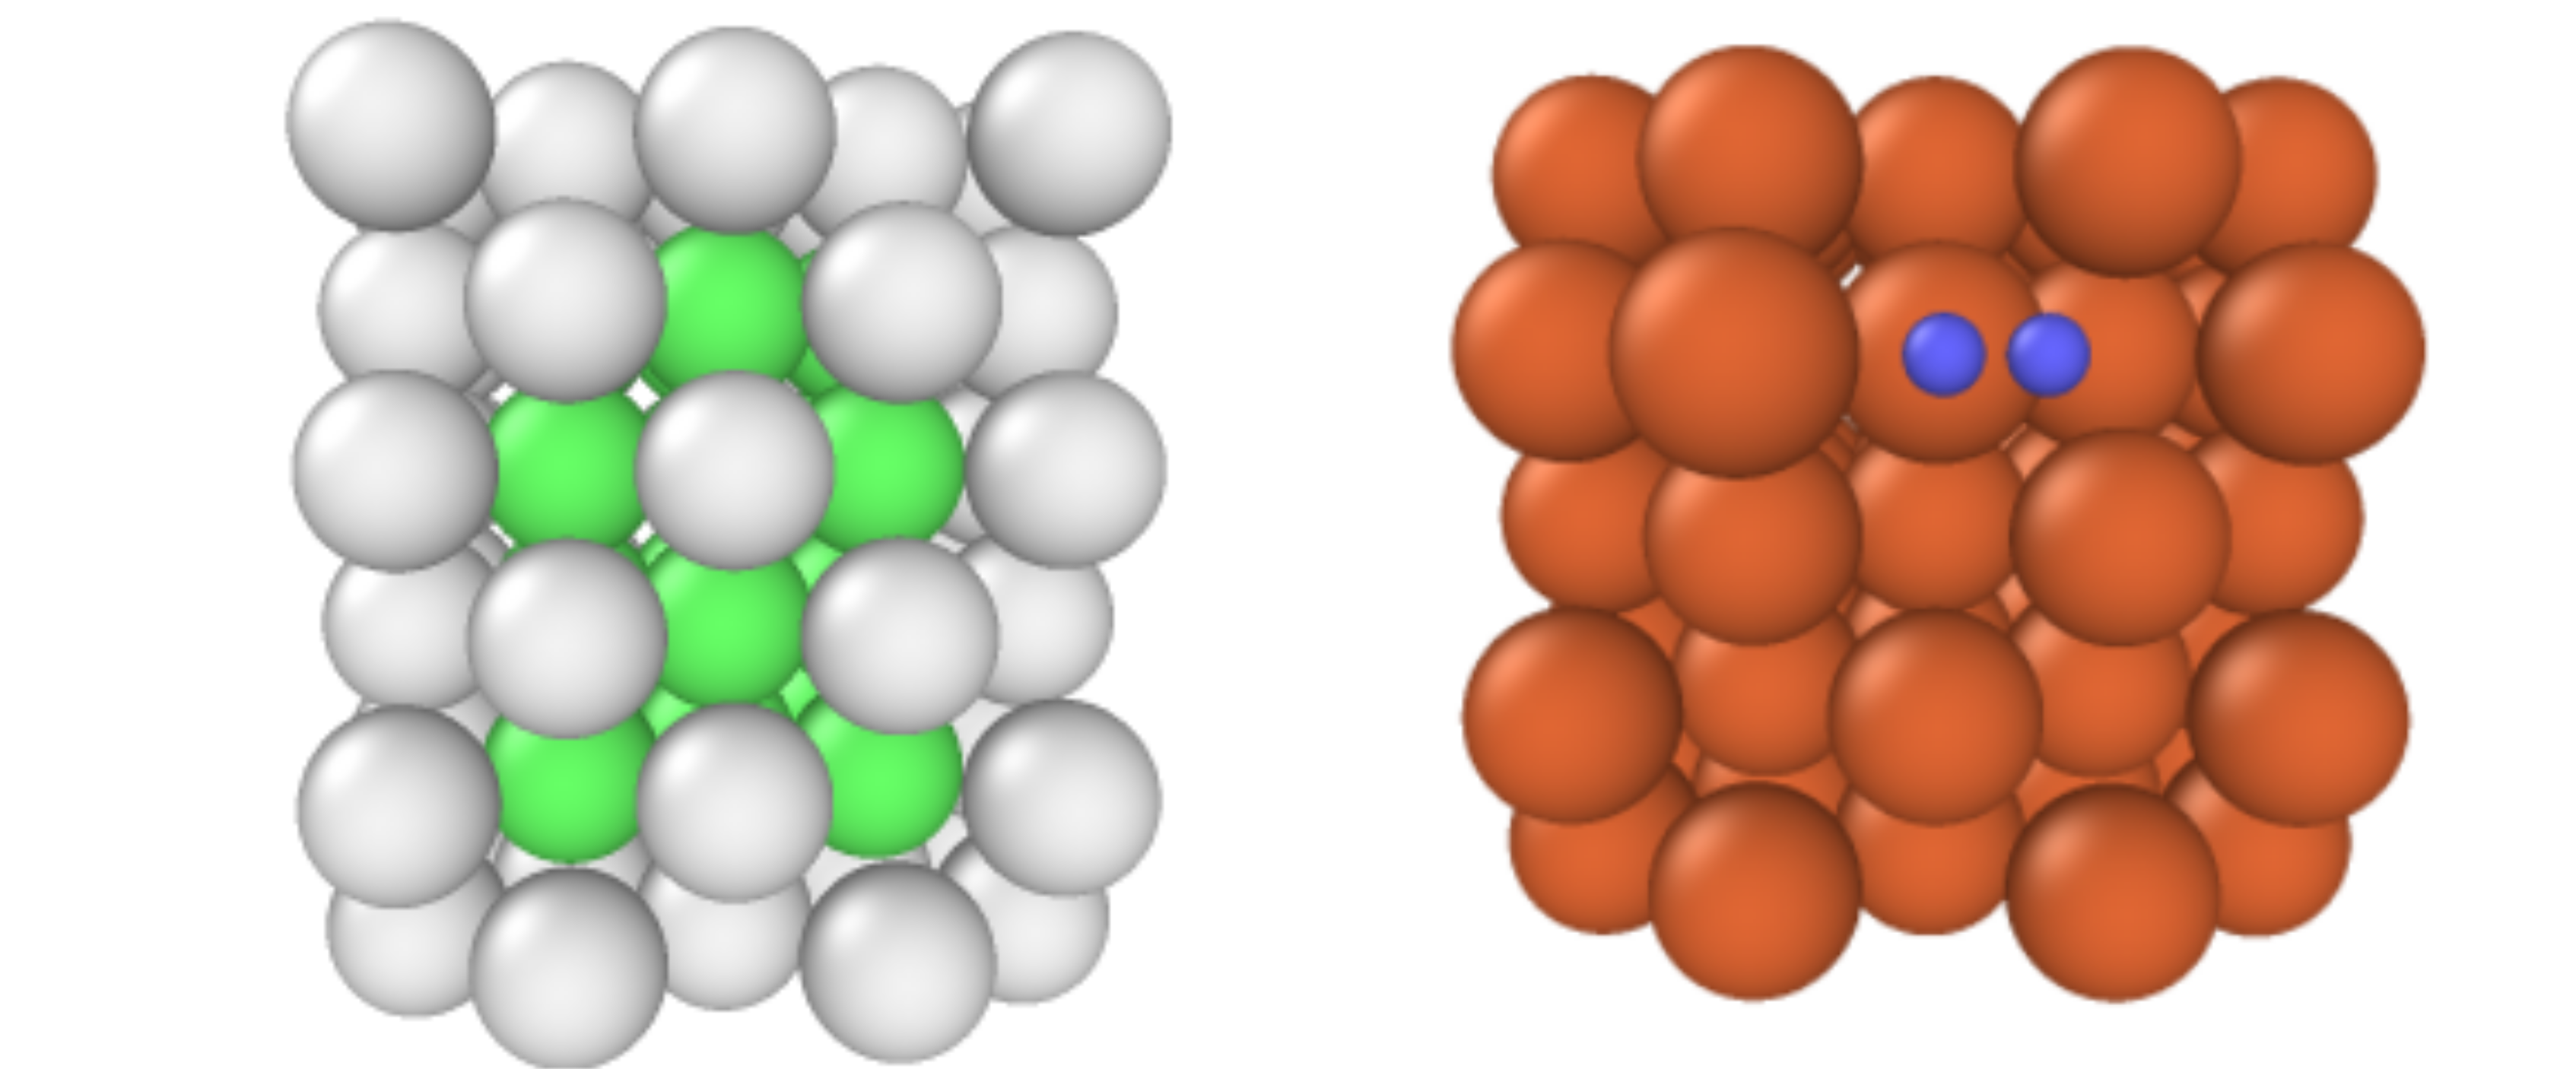
\includegraphics[width=\columnwidth]{./invariance/rec_examples/exrecal/combined.png}
\caption{(a) 75 atom cuboid cluster of face centered cubic (FCC) crystal. Green 
atoms are in an FCC environment, and have a complete set of FCC neighbours, grey atoms 
are surface atoms of the cluster and a have a lower coordination number.
(b) Same cluster with an extra bulk atom and two additional atoms 
placed on the surface at two different sites. 
\label{fig:cuboid}}
\end{center}
\end{figure}
%
The density of states in Fig.~\ref{fig:fcc_dos} is computed by 11 iterations of the 
recurrence equation. This generates continued fraction coefficients
from $a_{0}$ to $a_{10}$ and $b_{0}$ to $b_{11}$. 
A basis of five d orbitals are chosen to reside on each atom 
and their interaction via the Hamiltonian is determined by the Slater-Koster parameters.
The Hamiltonian parameters and the coefficients of the continued fraction are given in Table~\ref{tab:reccoeffs}.
The total DOS in this case is computed by combining the continued fractions computed for each of the 
five starting orbitals into a single continued fraction 
(multiple sets of continued fraction coefficients can be combined via the 
routine \texttt{RECSUM} in \texttt{CamRecLib}). 
%
\begin{figure}
\begin{center}
{\graphicspath{{./invariance/rec_examples/exrecal/}}\input{./invariance/rec_examples/exrecal/recal_dos.tex}}
\caption{Top panel: the local density of states on the central atom for the FCC 
cluster in Fig.~\ref{fig:cuboid} is computed. 
Bottom panel:  The contribution of the band structure to the 
cohesive energy and the integrated density of states.\label{fig:fcc_dos}}
\end{center}
\end{figure}
%

\begin{table}
\begin{center}
\begin{tabular}{|c|c|}
\hline
$a_{n}$ & $b_{n}$ \\
\hline
 0.000000E+00 & 0.100000E+01\\
-0.736283E-02 & 0.295643E-02\\
-0.296524E-01 & 0.178593E-02\\
-0.126548E-01 & 0.221181E-02\\
-0.225989E-01 & 0.178256E-02\\
 0.296606E-02 & 0.141733E-02\\
-0.129493E-01 & 0.196435E-02\\
-0.136124E-01 & 0.141377E-02\\
-0.170328E-01 & 0.181703E-02\\
-0.161681E-01 & 0.173104E-02\\
 0.000000E+00 & 0.148088E-02\\
\hline
\end{tabular}
\caption{Coefficients for the continued fraction DOS for a $d_{xy}$ orbital of a Ni 
atom in the middle of a small nickel cluster.\label{tab:reccoeffs}}
\end{center}
\end{table}

The difference in the qualities, in terms of the structure revealed, in the DOS 
is determined by the size of the cluster, the number of iterations of the
recurrence relations, the Hamiltonian, and the different termination 
scheme employed. 
\footnote{See the routines \texttt{DENCRS} and \texttt{DENSQ} 
for the square root and analytic terminator (TermDOS) schemes and \texttt{DENQD} 
for the QuadDOS termination scheme in the Cambridge Recursion Library 
\cite{nex84,haydock84,haydock85}.
The asymptotic behaviour of the continued fraction coefficients 
are affected by the presence of singularities
in the spectrum: e.g. band gaps, delta functions near the band edges,
the band edges themselves, and Van Hove singularities.
There is considerable literature on the topic of termination schemes 
and the analytic structure of the asymptotic coefficients:
\cite{hodges77,bylander80,turchi82,haydock84,luchini87,glanville88,
yoshino87,yoshino88,haydock89,haydock10,alhaidari18}.
In certain cases expressions for the behaviour of the coefficients
is given in terms of sinusoidal or elliptic functions. Linear prediction techniques
have also been used to study the behaviour of the recursion coefficients in the
asymptotic region \cite{allan84}. The problem of terminating the continued fraction
is quite an involved one and the discussion is deffered to the appendix.}

\subsection{Defects, Surface Electronic Structure and Orbital Peeling}
Surface catalysis is a topic of immense interest in chemistry and chemical engineering.
The rate at which reactions proceed is important in industrial and biomedical 
applications. The presence of a surface disrupts the periodicity required to use Bloch's theorem,
at least in the direction normal to the surface. In real systems
The periodicity parallel to the surface is also quite likely to 
be compromised by steps, terminating dislocation loops, 
vacancies and impurities. All this is to say that where 
there is a surface there is likely to be a need for recursion
techniques.

The need for a direct calculation of binding energy between adatoms or
the binding of a defect impurity in a lattice stems from the difficulties in computing 
these quantities via the method of energy differences. Performing two total
energy calculations on systems with on the order of $10^{23}$ atoms and subtracting the
resulting numbers is not a well conditioned problem. 
The very nature of the problem suggests that exploiting symmetries
will not greatly simplify things.

Relevant work on surfaces using the recursion method can be found in 
Refs.~\cite{haydock72, kelly73, kelly74, kelly74b, burke76, haydock79, haydock82}.
In particular \cite{haydock79} presents a quantitative treatment of chemisorption of simple
molecules to transition metal surfaces across the transition metal series. 
\footnote{This study provides a strong positive example of analysis of homologous 
trends in materials according to Ehrenreich's fourth point Chapter~\ref{chap:intro}}.
A detailed discussion of surface catalysis is also given in Ref.~\cite{haydock80}
for the dissociation of hydrogen on a transition metal surface. The apparent
connection to embrittlement phenomenon will be discussed in detail in Chap.~\ref{chap:metallurgy}.

The Cambridge Recursion Library provides an example 
to demonstrate some of the technique required to perform 
calculations of electronic properties on a surface. 

The example treats the problem of the interaction of adatoms on a 
surface, i.e. adatoms interacting via the metallic substrate.
The formalism was partially developed in Ref.~\cite{einstein73} and 
allowed for the study of adatom interaction energy 
as a function of the substrate band filling, adatom energy level, and the hopping
potential chosen between the adatom and the substrate. The generalization
to multiple orbital adatoms was given in Ref.~\cite{burke76}. 

The problem reduces to finding the difference in the total energy of the system when
adatoms are distant (infinitely separated) and when they are close together.
The total energy of the system is written:
%
\begin{equation}
U_{\rm TOT} = \sum_{i}\epsilon_{i} - U_{\rm ES},
\end{equation}
%
the first term is the band structure contribution to the energy, integrated
across all the occupied electronic states (on an adatom), and the second term is the electrostatic
energy, including the interelectron repulsion (to avoid double counting), and the repulsion
between the ion cores. It is the first term that is considered to be of primary 
interest in the example and corresponds to the energetic contribution coming 
from the adatoms sharing electrons via the d-band substrate.

The calculation proceeds as follows. First the two atoms are placed at a sufficient
distance that they do not interact and the energy:
%
\begin{equation}
U_{1} = \int_{-\infty}^{E^{(1)}_{F}}EN_{1}(E)dE,
\end{equation}
%
is computed. 

Then the two adatoms are allowed to come together on the surface, 
a new density of states is recalculated along with the new Fermi level.
%
\begin{equation}
U_{2} = \int_{-\infty}^{E^{(2)}_{F}}EN_{2}(E)dE,
\end{equation}

The integrals of the two density of states up to the two Fermi energies are equal
(no electrons have been added to the system).

The interaction energy can now be written:
%
\begin{equation}
W = \int_{-\infty}^{E_{F}} (E-E_{F})(N_{2}-N_{1}) dE
\end{equation}
%

The two reference systems are labeled System 1 and System 2. In Fig.~\ref{fig:burkesurf}
System 1 consists of two substrates each with an adatom, System 2 is a substrate with
2 adatoms and the empty substrate giving a Hamiltonian $H_{2}+H_{0}$.

The density of states then become:
%
\begin{equation}
N_{1} = 2{\rm Tr}[EI-H_{1}]^{-1}
\end{equation}
%
\begin{equation}
N_{2} = {\rm Tr}[EI-H_{2}]^{-1}
\end{equation}

Finally the identity: 
%
\begin{equation}
{\rm Tr}[EI-H]^{-1} = \frac{\partial}{\partial E} \log \det[EI-H],
\end{equation}
%
is employed to reach an expression for the difference in the density
of states $\delta N=(N_{2}-N_{1})$.
%
\begin{equation}
\delta N = \frac{\partial}{\partial E}\log\frac{\det[EI-H_{2}]}{\det [EI-H_{1}]}\frac{[EI-H_{0}]}{[EI-H_{1}]}
\end{equation}
%

What then follows is some consideration of the block structure of the matrices 
$H_2$, $H_1$ and $H_0$. $H_2$ is a partitioned matrix of dimension 
$5N+6$ and $H_1$ has dimension $5N+3$. $H_{0}$ is the substrate Hamiltonian 
with dimensions $5\times N$ (orbitals times atoms).
The self energy elements are given in the block $E_A$, $V_{1}$ and $V_{2}$ describe
the atoms interactions with the substrate and the $V_{12}$ describe the interaction
between adatoms. Some identities from matrix algebra employed in Ref.~\cite{einstein73}
and given in the appendix of Ref.~\cite{burke76} are then used to simplify the
expressions to:
%
\begin{equation}
\delta N = \frac{\partial}{\partial E}\log \frac{\det G_{1}}{\det G_{2}}
\end{equation}
%

The physical meaning is that $\log \det G_{2}$ gives the energy required to pull
one of two adatoms away from the substrate and its paired atom, the $\log \det G_1$
term is the energy required to put it back on substrate at an isolated site. 
The difference between these two energies is then the interaction energy. 
Formulating the problem as a matrix means the determinant can be split 
into a sum over five separate logarithms. This is accomplished by ``orbital peeling".

\begin{equation}
{\rm det}|G_{2}| = \bar{G}_{21}\bar{G}_{22}\bar{G}_{23}\bar{G}_{24}\bar{G}_{25}
\end{equation}

\begin{equation}
{\rm det}|G_{1}| = \bar{G}_{11}\bar{G}_{12}\bar{G}_{13}\bar{G}_{14}\bar{G}_{15}
\end{equation}

The matrix elements for each $G_{i\alpha}$ should be very familiar at this point:
%
\begin{equation}
G_{i\alpha}=\bra i,\alpha| [E-\bar{H}_{i\alpha}]^{-1} |i, \alpha\ket
\end{equation}
%
with $i=1,2$ $\alpha=1,5$. The matrix $\bar{H}_{i\alpha}$ is formed by taking 
$[E-\bar{H}_{i}]$, deleting the first $(\alpha-1)$ rows and columns 
to form $[EI-\bar{H}_{i\alpha}]$. The desired matrix element is now 
in the upper left-most corner of the matrix. 
Using this representation the difference in the density of states is calculated:
%
\begin{equation}
\Delta N = \sum_{\alpha=1}^{5} \frac{\partial}{\partial E}(\log\bar{G}_{1\alpha} - \log \bar{G}_{2\alpha})
\end{equation}
%

%
%The range of $E_{F}$ is restricted to $-0.068 \ge E_{F} \le 0.12$ Ryd by considerations
%based on the atomic configuration of tungsten as $5d^{4}6s^{2}$, meaning the band 
%should contain a minimum of 4 and a maximum of 6 electrons, with the band being half filled (5 e)
%considered the most plausible.

Fig.~\ref{fig:burkesurface} shows the energy difference as a function of the 
Fermi energy position. The energy is computed from the three p orbitals of a 
surface atom adhered to the same cluster studied in Sec.~\ref{sec:fccldos}.
%
\begin{figure}
\begin{center}
{\graphicspath{{./invariance/rec_examples/exorpeel/}}\input{./invariance/rec_examples/exorpeel/exorpeel.tex}}
\caption{Top panel: Adsorbate interaction energy as a function of the Fermi energy for a representative d band
substrate. Mutual interaction of the adsorbates is mediated by the substrate and the p-d surface interaction.
Interaction goes to zero when the substrate band is completely filled. 
Bottom panel: Difference in the total energy for the two adsorbate configurations as a function of
d-band filling (position of the Fermi energy). See Ref.~\cite{burke76} for details. \label{fig:burkesurface}}
\end{center}
\end{figure}
%

These early surface calculations using the recursion method were overwhelmed 
by a number of uncertainties. The lack of a procedure for a choice of the tight-binding 
Hamiltonian and difficulties in accessing the self consistent charge density
and relaxed configurations in the presence of a surface being the most significant.
\footnote{For early work on Wannier functions at surfaces Ref.~\cite{smith74}. Also see 
\cite{mostoller79} for a treatment of surface effects using the recursion method.}

The development of first principles calculations 
has greatly simplified access to these quantities and should remove 
some of the ambiguities in mapping ab initio data onto a local picture
of the electronic structure at surfaces. These advances mean that the 
recursion techniques described in Refs.~\cite{burke76, haydock79, haydock81} 
might be revisited with potentially profitable effect. 

For applications of orbital peeling to defects and the 
computation of interaction energies and variations in the charge density
see Refs.\cite{gibson93,gibson94}. However that work partially relies 
on the computation of off diagonal of the Green's function. A topic
to which we turn now.

\subsection{Off-Diagonal Elements of the Green's Function}
The off-diagonal elements of the Green's function can be written:
%
\begin{equation}
G_{AB}(E) = \bra \phi_{A}|[H-E]^{-1}|\phi_{B}\ket,
\end{equation}
%
and they contain a lot of useful information. 

These off-diagonal elements are required to calculate 
response functions, \cite{terakura78}, interatomic 
forces \cite{finnis84, finnis87, ohta87}, and bond orders 
\cite{coulson39,tersoff86,pettifor89}.

One direct route to computing an off-diagonal elements of the Green's function
is by expressing it as a linear combination of two diagonal elements. 
This can be seen by forming new starting vectors 
from the potential linear combinations of $\phi_{A}$ and $\phi_{B}$:
%
\begin{align}
\phi_{+} = \frac{1}{\sqrt{2}}(\phi_{A} + \phi_{B})\\
\phi_{-} = \frac{1}{\sqrt{2}}(\phi_{A} - \phi_{B})\\
\phi_{i+} = \frac{1}{\sqrt{2}}(\phi_{A} + i\phi_{B})\\
\phi_{i-} = \frac{1}{\sqrt{2}}(\phi_{A} - i\phi_{B}),
\end{align}
%
we can retrieve the off-diagonal elements by computing 
two `normal' diagonal elements from these linear combinations.
For example, for an Hermitian $\hat{H}$, and real $\phi_{A}$ and $\phi_{B}$ 
the $AB$ off-diagonal element of the Green's function can be computed as:
%
\begin{equation}
\label{eq:offdiaggreen}
G_{AB}(E) = \frac{1}{2}[G_{++}(E)-G_{--}(E)].
\end{equation}

\subsection{The Tight Binding Bond Model}
To see how the off-diagonal elements contribute to the force on an 
atom we follow Sec. 2.4 of Sutton \cite{sutton88} and Ohta \cite{ohta87}.
First we reproduce their expression for the bond energy:
%
\begin{equation}
\label{eq:tbenergy}
u_{ij} = u^{\rm rep}_{ij} - \frac{4}{\pi}\sum_{\lambda\mu} 
h_{ij}^{\lambda\mu}{\rm Im}\int_{-\infty}^{\epsilon_{F}}G_{ji}^{\mu\lambda}(\epsilon+i0)d\epsilon,
\end{equation}
%
The total energy is then a sum over the bond energies:
%
\begin{equation}
\label{eq:tbtoten}
U^{\rm tot} = \frac{1}{2}\sum_{ij,(i\neq=j)}u^{\rm tot}_{ij}
\end{equation}
%

The expression for the bond force follows naturally as the gradient of the bond energy:
%
\begin{equation}
\label{eq:tbforce}
f_{ij}^{\alpha} = f^{\rm rep}_{ij\alpha} - \frac{4}{\pi}\sum_{\lambda\mu} 
\nabla_{i\alpha}h_{ij}^{\lambda\mu}{\rm Im}\int_{-\infty}^{\epsilon_{F}}G_{ji}^{\mu\lambda}(\epsilon+i0)d\epsilon,
\end{equation}
%
$\alpha$ is a Cartesian direction, $i,j$ are site indices, and $\lambda, \mu$ are orbital indices 
the z axis lies along the bond connecting atoms i and j. The first term in Eq~\ref{eq:tbforce} 
we will come back to this term in Chapter~\ref{chap:gw} and Chapter~\ref{chap:wannier}. 
It is very much a term determined by craft and describes the repulsive contribution of the ion cores. 
But all this to come. 

For now it is the second term that is of interest and
it is easily recognized as something we can access via the Green's function 
computed using recursion techniques. It is also important to note that 
Eq.~\ref{eq:tbforce} is certainly not a two body interaction! The Green's function 
as it is calculated accounts for information from every shell of neighbours 
until there are no more or the recursion process is terminated. 
The importance of this local formulation of forces should not be underestimated.
Many of the practical applications discussed in Chapter~\ref{chap:metallurgy} 
will rely on it.

%
These off-diagonal elements are also required to determine the vibrational properties. 
If we want the interatomic force constants determining the harmonic energy surface 
we follow Finnis\cite{finnis84} and go to second order in the variation of the 
total energy to derive the interatomic force constant matrix:
%
\begin{equation}
\label{eq:tbdynmat}
\psi_{\alpha\beta}^{ab} = \hat{\psi}_{\alpha\beta}^{ab} +  \sum_{dnq\sigma}(\delta 
\rho_{bd,a\alpha}^{nq,\sigma}\nabla_{\beta}h_{db}^{qn} + \delta\rho_{ad,b\beta}^{nq,\sigma}\nabla_{\alpha}h_{da}^{qn}),
\end{equation}
%
$h^{qn}_{db}$ is a two center hopping integral that links the orbital n on atom b to orbital 
q on atom d. For the d electrons this integral is taken to decay as
$\r^{5}$. The density changes are proportional to the variation in the Hamiltonian 
multiplied by the response function. Displacing atom a in the $\alpha$ direction induces a change in the
bond charges about atom b. The change in the bond charge between atoms b and d 
in the spin-$\sigma$ channel stemming from orbitals n and q is then given by:
%
\begin{equation}
\label{eq:tbdeltarho}
\delta \rho_{bd,a\alpha}^{nq,\sigma} = \sum_{cmp}(\chi_{bc,ad}^{np,mq,\sigma}+\chi_{ba,cd}^{nm,pq,\sigma})\nabla_{\alpha}h_{ac}^{pm}
\end{equation}
%
where the response function is defined as:
%
\begin{equation}
\label{eq:tbresponse}
\chi_{bc,ad}^{np,mq,\sigma} = \frac{1}{\pi}{\rm Im}\int^{E_{F}}G_{bc}^{np,\sigma}(\epsilon)G_{ad}^{mq,\sigma}(\epsilon)d\epsilon,
\end{equation}
%

An interesting relationship can be derived between off-diagonal elements
and the response functions \cite{terakura82, sutton88}:
%
\begin{equation}
\frac{dG}{dE}=-G^{2},
\end{equation}
%
and upon integration:
%
\begin{equation}
\frac{-2}{\pi}G_{jk}(E^{+}) = \frac{2{\rm Im}}{\pi}\int^{E}\sum_{l}G_{jl}(E')G_{lk}(E')dE'.
\end{equation}
%

Fig.~\ref{fig:tbresponse} gives a pictorial representation of some of these many indiced terms. In 
Ref.\cite{finnis84} the Green's functions are computed out to sixth nearest neighbour. This allows
for force contributions out to the thirteenth nearest neighbour. Symmetry relations are exploited 
in that work to reduce the number of unique off-diagonal Green's function elements to 
33 separate functions which are tabulated and used to compute the force constant matrix. 
%
\begin{figure}
\begin{center}
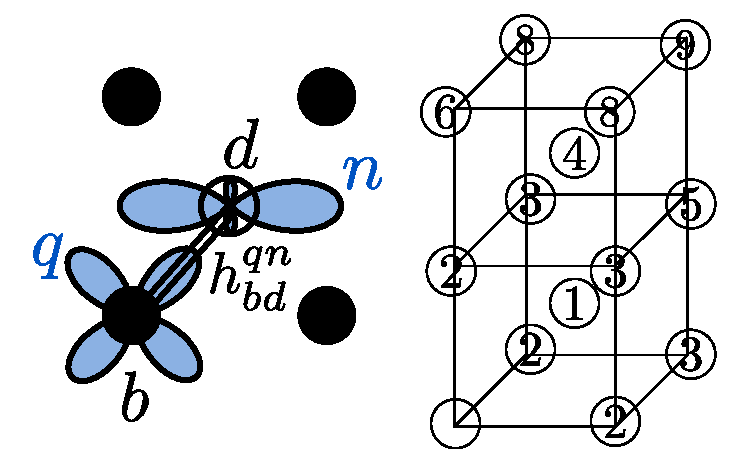
\includegraphics[scale=0.8]{./invariance/tbresponse.pdf}
\caption{Pictorial representation of the terms and sites 
described by Eq.~\ref{eq:tbdynmat}. On the left atoms $b,d$ 
and two orbitals centered on those sites, $n, q$, and the energy
integral $h_{bd}^{qn}$ which connects them. On the right are two unit cells
of BCC crystal with the nearest neighbours to the zeroth atom 
labeled out to its sixth nearest neighbour.\label{fig:tbresponse}}
\end{center}
\end{figure}

The type of analysis in Ref.~\cite{finnis84} is taken as an example
of the desired computational framework these notes pursue. 
The approach satisfies many of Ehrenreich's points ~\ref{en:ehrenreich}: 
direct experimental links, tractable calculations 
for a minimally idealized system, and, most importantly, 
the calculations have {\emph explanatory and predictive power 
across a homologous series}, in this case the BCC transition metals.
\footnote{For neutron spectroscopy data determining vibrational modes 
see \cite{powell68, colella70, shaw71}, The mystery of obtaining a 
good experimental phonon spectra in published literature continues... 
A. M. B. G. De Vallera, Ph.D. thesis, Cambridge University, 1977 (unpublished).
However it is apparently quite similar to NbMo\cite{powerll68}.}

The only point not fully satisfied is that of theoretical justification.
The force constants as determined in Eq.~\ref{eq:tbdynmat}
rely on the repulsive force and some means of determining 
the local Hamiltonian i.e. its bond integrals and their 
radial dependence {\it ab initio}. Addressing these issues
will be the subject of subsequent chapters. 
 
Eqs.~\ref{eq:tbdynmat, eq:tbdeltarho, eq:tbresponse} encode
a huge amount of information. Although well developed reciprocal space 
techniques exist, see Ref.~\cite{baroni01}, to obtain the phonon dispersion
curves, the local formulation still has a great deal of 
interprative value, and crucially, will remain valid
in situations where Bloch's theorem does not.

The bond order between atoms has a long history
beginning with Coulson's study of carbonyl 
chains in Ref.~\cite{coulson39,coulson47}. 
It is a good exercise to compare the derivative of Eq.~\ref{eq:tbtoten} with respect
to the hopping integral and the Green's function,
with Coulson's definition of the bond order\cite{coulson39}. 
The correlation of the experimental data in the form of bond lengths
with the concept of a bond order in polyenes and aromatic molecules
is an elegant demonstration of a theory and application closely
linked to experimental data, and studying the trend in a property
of homologous materials.

\footnote{The obituary of C.A.Coulson\cite{altmann74} 
is highly recommended reading. His obituary gives an insight into 
of how wave mechanics was imported to the study of 
complex molecules and crystals at the earliest stage. Coulson's 
immense contribution to the study of electronic structure
begins near the inception of quantum theory. As mentioned in Ref.~\cite{altmann74}
Coulson is supposed to have attended a seminar given by Dirac 
where Dirac was discussing the uncertainty relation: $xp-px=ih$.
When Coulson inquired when this work had been done Dirac replied, 
``Last night." In 1938 Coulson may have performed the first 
iterative self-consistent field calculations 
on a molecule, $H_2$, by hand (with the possible help of a £25 Brunsviga calculator)
~\cite{coulson38}. Coulson's life work spans diverse fields.
A small selection from his bibliography will find work 
touching on numerical methods \cite{coulson37,coulson42}, 
random walks with an application to a certain type of slug 
traversing a surface in the presence of a bright light \cite{coulson47}, 
the electronic structure of aromatic compounds and polymers, 
dielectric media, and theology. The application of the methods 
reviewed in the present work to his fields of endeavour would 
constitute a textbook onto itself.}

The order of a given bond is a measure
of the force tending to change the length of a given bond
for small variation of the bond length.

Defined in terms of Green's functions, the bond order is the integrated 
energy difference between a symmetric and anti-symmetric combination 
of nearest neighbour orbitals \cite{pettifor89}:
%
\begin{equation}
\label{eq:bondorder}
\Theta_{ij} = - \frac{2}{\pi} {\rm Im} \int^{E_{F}}\left[G^{+}_{00}(E)-G_{00}^{-}(E)\right]dE.
\end{equation}
%
The bond order in this form then appears like a measure of the interference 
between orbitals on the two sites.

As we integrate up in energy the difference in the symmetric and antisymmetric 
combinations of the two states are accumulated. The resulting integral is 
then a scalar which measures the sign and magnitude of the
interference between the two localized orbitals up to the Fermi energy.

Eq.~\ref{eq:offdiaggreen} gives an immediate scheme for computing the 
off-diagonal elements but can result in the need for substracting 
two largish quantities to find a small one. Such a procedure 
is never ideal. This concern and others motivated the introduction
of the block recursion method which will be discussed shortly.

First though a small digression.

Harrison in his textbook argues that every conclusion drawn in 
his work follows immediately from the proposition that electrons 
are simultaneously a particle and a wave. 
In the context of the recursion method we can propose 
a tentative meaning to his statement: the electron is a 
particle when we can point to it and say, `There it is. 
It is in that orbital centered on that atom.' It becomes a wave 
when the recursion process is initiated and the spectral weight of the 
localized orbital spreads outwards onto neighbouring atoms. 
The form this interaction takes in the recursion method 
is the linear mixing of the starting vector
with the other localised vectors in the system from 
further and further away, adding these vectors with changing coefficients,
allowing them to interfere constructively or deconstructively. 

When the recurrence is terminated a record of the projection of 
the starting orbital on to each of its increasingly distant neighbours 
is recorded. The electron, though confined to a discrete energy 
and state on the lone atom, when placed in a solid, can 
take on a range of shapes across a range of energies distributed 
throughout a crystal.

\subsection{Non-Orthogonal Recursion}
\label{sec:tensornotation}
The underlying assumption about the basis vectors
used to describe the system up to this point have 
been that they are orthogonal. However the most intuitive basis set to 
choose, a basis of atomic orbitals centered on an atom, 
the original choice made by Bl\"och, will not be orthogonal. 

L\"owdin functions are a class of localized orthogonal functions,
as are Wannier functions but the price to be paid for
obtaining these functions is often that of an entire 
first principles calculation. These matters will 
be discussed further in Chap.~\ref{chap:wannier}.

Anderson's chemical pseudopotential theory is formulated 
in terms of a generalized eigenvalue problem \cite{anderson68,anderson69}
as are the molecular building block type orbitals of \cite{edmiston63} 
and the work of Boys and Boys and Foster~\cite{boys60a,boys60b}. 

Though we begin to digress it is clear that for physical 
and numerical accuracy we require an orthogonal basis 
set but for intuition or heuristic purposes we may wish to continue thinking
in terms of nicely formed localized starting states that 
are not orthogonal but easy to picture and initialize.

In any case when the basis vectors set up to describe the system
are not orthogonal some choices need to be made. There are two options.
The most tempting option is just to ignore the non-orthogonality of the
vectors and carry on. The other is to modify our approach somewhat. 
The latter course is the morally upright one. 

If the basis set for the Hamiltonian is given as a set of
${\phi_{m}}$ orbitals elements of the overlap matrix can 
be written:
%
\begin{equation}
[S]_{mn} = \int \phi^{*}_{m}(\r)\phi_{n}(\r)d\tau
\end{equation}
%

Given two states $\mathbf{u}$ and $\mathbf{v}$ which
are linear combinations of the $\phi$ the physical
overlap of the states is given: $\mathbf{v}^{\dagger}S\mathbf{u}$.

The Hamiltonian operator $\mathcal{H}$ acts on a basis orbital and
its effect is approximated by a sum over the basis orbitals:

\begin{equation}
\mathcal{H}\phi_{n}(\mathbf{r}) = \sum_{n=0}^{\infty} H_{mn}\phi_{m}(\r)
\end{equation}

If the basis set is not orthogonal the Hamiltonian operator
is related to its representation in the basis set as:

\begin{equation}
\mathcal{H}_{mn} = [SH]_{mn}
\end{equation}

In the cases where S and $[\mathcal{H}_{mn}]$ are known the Hamiltonian
matrix is required which is obtained from:
%
\begin{equation}
H = S^{-1}[\mathcal{H}_{mn}],
\end{equation}
%
this transformed matrix is sometimes denoted $D$ in the literature
see Ref.~\cite{weeks73} for a discussion of the properties of
this transformed Hamiltonian. S should hopefully have some 
nice properties like its diagonal elements are unity and that it 
possesses small off-diagonal elements that fall off relatively 
quickly in real space.

The previous notation follows Haydock's article in Vol. 35 and uses 
a calligraphic $\mathcal{H}$ to denote the Hamiltonian operator and 
a roman $H$ with subscripts to denote the matrix elements of this operator 
projected onto the chosen basis set. 

In Ref.~\cite{ballentine86} Ballentine and Kol\'a\'r introduced 
a compact tensor notation to keep track of whether one was working 
with matrix elements of the overlap matrix and Hamiltonian 
in the non-orthogonal basis or in the Hamiltonian transformed by
the overlap matrix. The call to follow this tensor notation 
was echoed in Ref.~\cite{sutton88} and we describe it here to help
clarify the implementation of the non-orthogonal recursion method.
In Ref.~\cite{foulkes86} this notation was exploited in order to 
study some extensions of the recursion method to the evaluation of 
operator matrix elements. A transparent notation can greatly clarify
the concepts.

In what follows the lower case greek letters in the sub and superscripts
denote a composite orbital index comprised of the site-index and the 
angular momentum channel. In later sections of this chapter this notation
might be expanded with site indices denoted using lower case
roman letters and orbital indices denoted by lower case greek letters.
An effort is made to use $\alpha$ and $\beta$ where the index is a composite
one and $\lambda$, $\mu$, where they refer only to orbital indices with the 
site index made explicit. The usage should be clear from the context.

The matrix element of the overlap between non-orthogonal 
basis functions can be written:
%
\begin{equation}
S_{\alpha\beta} = \bra \psi_{\alpha}|\psi_{\beta}\ket
\end{equation}
%
with $i,j$ referring to a site index and $\alpha$ and $\beta$ 
referring to orbital indices.

The matrix elements of the Hamiltonian with the non-orthogonal states takes
the form:
%
\begin{equation}
H_{\alpha \beta} = \bra \psi_{\alpha}|H|\psi_{\beta}\ket
\end{equation}

The inverse of the overlap matrix is defined:
%
\begin{equation}
\sum_{\beta}(S^{-1})^{\alpha\beta}S_{\beta\gamma}=\delta^{\alpha}_{\gamma}.
\end{equation}
%

Naturally, the elements of the inverse overlap matrix $S^{-1}$ are chosen 
such that they produce the identity matrix upon multiplication $S$.

The dual set of basis vectors is:
%
\begin{equation}
|\psi^{\alpha}\ket = \sum_{\beta}|\psi_{\beta}(S^{-1})^{\beta\alpha}.
\end{equation}
%
If the overlap matrix is just the identity matrix the original 
basis set is already orthonormal and the dual vectors (covariant
contravariant, or upper and lower indiced, depending
on your naming preference) are equal.

The two most important aspects of any basis set
are {\it representation} and {\it normalization}. 
We can reprsent an arbitrary vector $|u\ket$:
%
\begin{equation}
|u\ket = \sum_{\alpha}u^{\alpha}|\psi_{\alpha}\ket = \sum_{\alpha}u_{\alpha}|\psi^{\alpha}\ket.
\end{equation}
%
The expansion coefficients in either basis can be obtained via:
%
\begin{equation}
u_{\alpha} = \sum_{\beta}S_{\alpha\beta}u^{\beta}.
\end{equation}
%

Along with {\it representation} we require a {\it norm} i.e. 
the inner product of two vectors:
%
\begin{equation}
\bra v|u \ket = \sum_{\alpha\beta}v^{\alpha *}S_{\alpha\beta}u^{\beta} = \sum_{\alpha}v^{\alpha *}u_{\alpha} = \sum_{\beta}v_{\beta *}u^{\beta}
\end{equation}
%

The Hamiltonian in a mixed representation takes the form:
%
\begin{equation}
\label{eq:mixedH}
H^{\alpha}\ _{\beta} = \sum_{\gamma}(S^{-1})^{\alpha\gamma}H_{\gamma\beta}.
\end{equation}
%
This form of the Hamiltonian matrix is sometimes referred to as $D$ \cite{weeks73}.

The reason for going to all this trouble of defining upper and lower
indexed vectors and a tensor notation is illustrated by considering how the Schr\"odinger
equation looks in different representations. If one works with
the easily instantiated, in the sense that one has the Hamiltonian and
overlap matrix elements to hand, but non-orthogonal basis set the Schrodinger
equation takes the form:
%
\begin{equation}
H..\psi^{\mbox{\large .}}=\epsilon S..\psi^{\mbox{\large .}}
\end{equation}
%

However if the Hamiltonian is converted to the mixed representation:
%
\begin{equation}
H^{\mbox{\large .}}.\psi^{\mbox{\large .}}=\epsilon\psi^{\mbox{\large .}}
\end{equation}
%
the overlap matrix disappears and the eigenvalue problem is in a 
more familiar form. The Hamiltonian in the mixed representation 
is that obtained from Eq.~\ref{eq:mixedH}. The price? The Hamiltonian
is no longer necessarily Hermitian.

The starting vector for the recursion will often be a lower indiced
vector corresponding with the basis set chosen to represent the electron
states.

Ballentine and Koclar conclude by giving the trace of an operator:
\begin{align}
{\rm Tr}A =& \sum_{\alpha\beta}S_{\alpha\beta}A^{\beta\alpha}\\
          =& \sum_{\alpha\beta}(S^{-1})^{\alpha\beta}A_{\beta\alpha} \\
          =& \sum_{\alpha}A^{\alpha}_{\alpha}
\end{align}

The trace of the Hamiltonian or density operator would be necessary 
if one wished to compute, for example, the total band energy 
or the density. Depending on which matrix elements one has to hand, 
the lower indiced being the more accessible generally. 

As mentioned the trouble with the mixed representation of the Hamiltonian is,
although it escapes the need to deal directly with the overlap 
matrix or its inverse, it is no longer Hermitian. 

The following two subsections suggest a generalization of the recursion
scheme to deal with non-Hermitian matrices, and a practical means
of performing non-orthogonal calculations which exploit the Gauss-Seidel
iterative scheme to obtain the inverse of the overlap matrix efficiently.
In effect these two approaches amount to the choice of working
in the mixed representation or working with the inverse of the overlap
matrix and the lower indiced Hamiltonian respectively.

\subsubsection{Two-Sided Lanczos}
For the case where $H\neq H^{*\dagger}$ i.e. for a non-Hermitian
Hamiltonian a two-sided Lanczos algorithm exists as discussed in
Ref.\cite{haydockkelly75} following Wilkinson's description.

Two starting vectors are chosen $|u_{0}\ket=|0\ket$, $|v_{0}\ket=|0\ket$
and two chains of recurrences are generated:
%
\begin{equation}
b_{n+1}|u_{n+1}\ket = H|u_{n}\ket - a_{n}|u_{n}\ket - b_{n}|u_{n-1}\ket
\end{equation}
%
\begin{equation}
b_{n+1}|v_{n+1}\ket = H^{\dagger}|v_{n}\ket - a_{n}|v_{n}\ket - b_{n}|v_{n-1}\ket
\end{equation}
%
where $a_{n} = \bra v_{n}|H|u_{n}\ket = \bra u_{n}|H^{\dagger}|v_{n}\ket$
and the overlap is given by $b^{2}_{n+1} = \bra v_{n+1}|u_{n+1}\ket$.

The danger of the two sided recursion algorithm is that the inner
product of the vectors $\bra v_{n+1}|u_{n+1}\ket$ could become negative.
The density of states would no-longer be non-negative which makes it
more difficult to interpret as a local density of states. The fact 
that the Hamiltonian is non-Hermitian does not guarantee this will 
be the case so the application of this method may not produce 
any complex eigenvalues. S. F. Boys has given a thorough treatment
of the convergence properties of non-Hermitian operators in Ref.~\cite{boys69}.

\subsubsection{\texttt{RECNO}: Recursion Non-Orthogonal Algorithm}
The approach to the \index{non-orthogonal basis vectors} taken in the 
\texttt{CamRecLib} routine \texttt{recno} is slightly different.
It is similar to the approach taken in Refs.\cite{jones84, jones85} which
uses the Gauss-Seidel method or the Cholesky decomposition
to efficiently compute the application of the inverse of the overlap matrix
and obtain the $H^{\alpha}_{\beta}$ of the Hamiltonian discussed in 
Section~\ref{sec:tensornotation}.

Following the notation in \cite{nex89} the generalized 
eigenvalue problem to be solved becomes:

\begin{equation}
MX = \epsilon S X
\end{equation}

The actual Greenian computed is:
%
\begin{equation}
\bra u_{0}S|[S\epsilon-M]^{-1}|Su_{0}\ket
\end{equation}
%

The \texttt{RECNO} algorithm then proceeds according to the following steps:
%
\begin{flalign}
\psi_{0} = & Su_{0} \\
b^{2}_{1} = & \bra u_{0}|\psi_{0} \ket \\
\end{flalign}
Then up to the $LL^{th}$ iteration of the recurrence:
\begin{flalign}
 a_{n} = \frac{\bra u_{n}|M u_{n}\ket}{\bra u_{n}|\psi_{n} \ket}&\\
 \psi_{n+1} = M u_{n} - a_{n}\psi_{n} - b^{2}_{n}\psi_{n-1}&\\
 u_{n+1} = S^{-1}\psi_{n+1}&
\end{flalign}
%
The Gauss-Seidel Algorithm \index{Gauss-Seidel} is used 
to compute the application of the inverse 
of the overlap matrix to the recursion vector so $S^{-1}\psi_{n+1}$:
%
\begin{equation}
u_{n+1}^{i} = \psi_{n+1} - Lu_{n+1}^{i} - Ru^{i-1}_{n+1}
\end{equation}
%
L and R are the strict left and right triangular parts of S.

In Ref.~\cite{weaire85} R. Jones proposes an alternative strategy
for obtaining and applying the inverse matrix $S^{-1}$ based on the Cholesky
decomposition \index{Cholesky Decomposition}.

A lower triangular matrix $L_{ij}$ is calculated by solving:
%
\begin{align}
\label{alg:cholesky}
L_{ll} = & \sqrt{S_{ll}}   &\\
S_{il} = & L_{il}L_{ll}    & i>l\\
S_{ij} = & \sum_{k \leq j}L_{ik}L_{jk} & j\leq i
\end{align}

$U_{i}$ in Eq.~\ref{eq:} is then found by solving for $q$:
%
\begin{equation}
\sum_{k\leq i} L_{ik}q_{k} = \psi_{i}
\end{equation}
%

followed by:
%
\begin{equation}
\sum_{k\leq i} L_{ik}U_{k} = q_{i}
\end{equation}
%
using back substitution. 

For ease of reference we also write out the explicit expressions 
for the elements of $L$ determined in the Cholesky decomposition:
%
\begin{align}
L_{jj} =& \sqrt{S_{jj} - \sum_{k=1}^{j-1}L_{jk}L^{*}_{jk}}\\
L_{ij} =& \frac{1}{L_{jj}}(S_{ij}-\sum_{k=1}^{j-1}L_{ik}L^{*}_{jk})
\end{align}
%
The forward substitution can proceed column wise or row wise. 
See Ref.~\cite{wilkinson68} for a discussion of the 
stability of this procedure.

Both the Gauss-Seidel and Cholesky processes emphasise the physical consequence
of applying $S^{-1}$ to the recursion vector at each step.
It is like a small orthogonalizing hair-cut applied at each stage of the recurrence
to remove the double counting of components that would arise 
as a consequence of the overlap of the basis set. The more 
diagonally dominant the overlap matrix is the faster the Gauss-Seidel 
algorithm will converge.

\subsection{Block Recursion}
The block recursion method is a direct and intuitive extension of the scalar method.
In this method a {\emph set of m} initial orbitals are chosen. The recursion
coefficients then become matrices, and the continued fractions become
matrix continued fractions. The technique and its implementations are described 
in Refs.~\cite{jones84, legrand85, inoue87, nex89, godin91}. 
The applications of the block recursion method are varied.
Lewis and Jones in Ref.~\cite{jones84} derived the block recursion method
in order to compute the real space electron density from a basis of atomic orbitals.
Paxton's study of the stability of different phases of silicon in 
Refs.~\cite{paxton87, paxton88} required the block recursion method so that
the computed Greenians respected the underlying rotational symmetries of the 
Hamiltonian. This point will be discussed more shortly. The work of 
Godin and Haydock focused on the ability of the block recursion technique
to directly provide off diagonal Greenians required for quantum transmittance problems
on the passage of electrons through disordered media in Refs.~\cite{godin86, godin88}. 

The notation we supply here is a synthesis of the descriptions 
given in Refs.~\cite{paxton88, nex89} and is in 
accord with the accompanying \texttt{CamRecLib} routines.

We make a simple adjustment to the notation when discussing
block recursion as opposed to scalar recursion.
The starting vector $u_{0}$ and the recursion coefficients
$a_{n}$ and $b_{n}$ from the scalar case are transformed to
matrices denoted by capital letters $U_{0}$, $A_{n}$, and $B_{n}$
in the case of block recursion. Where recursion coefficents could be
inverted by simple division the block matrices require matrix inversion.

\subsubsection{Transforming Like a Tensor}
By picking a single orbital and turning the wheel on the recursion method a
chain of coefficients and vectors can be generated. However rounding errors in the evaluation
of the matrix vector products mean the accumulation of numerical noise
generated by the artifical truncation of the recurrence
can disrupt underlying symmetries. This can be demonstrated where there are 
deviations in the density of states computed for a given orbital if the z-axis 
is changed For some historical insight into the need for block recursion formulation
we quote from Finnis' article in Ref.~\cite{andersen89}:

\begin{quote}
The first problem came to our attention in the course of 
calculating the relaxed structure of a (310) grain boundary.
The potential had been adjusted to ensure that the perfect lattice
was in equilibrium at zero pressure with the observed lattice constant. Yet
when the perfect lattice was reoriented to set up the (310) grain boundary, the 
perfect part of the structure was no longer in equilibrium! Our forces were not transforming
properly as vectors under rotations. In fact, neither was the energy rotationally invariant.
The cause of the problem was that although the exact Green function would transform as a tensor,
the approximate Green function matrix elements obtained by termination or quadrature
methods do not transform exactly into their symmetry related combinations under lattice 
rotations.
\end{quote}

Inoue and Ohta addressed the former problem, i.e. the proper transformation of the forces,
in their formulation of the block recursion method\cite{inoue87}. 
It is useful to incorporate their discussion of the underlying 
symmetries of the Green's function and Greenians.

Their notation follows Edminson, where a rotation of the co-ordinate axis
of the system by the Euler angles $\alpha$,$\beta$, and $\gamma$ is denoted:

\begin{equation}
R(\alpha\beta\gamma)H
\end{equation}

If the crystal under considerations has a potential V which transforms as some symmetry group
the Slater-Koster matrix elements will also transform according to that symmetry group:
%
\begin{equation}
H_{i\lambda j\mu} = \bra \phi_{i\lambda} | -\frac{\hbar^{2}}{2m}\nabla^{2} + V|\psi_{j\mu} \ket
\end{equation}
%

%
We may denote the action of an element of the symmetry group of the crystal $G_{h}$ by:
%
\begin{equation}
G_{h} H_{ij} =  K^{\dagger}(h)H_{ij}K(h)
\end{equation}
%
where $K(h)$ is a matrix representation of the symmetry element 
with respect to the atomic orbitals. 

\subsubsection{The Block Recursion Algorithm}
\label{sec:blockrecursion}
\index{blockrecursion}
The matrix Greenian to be computed is:
\begin{equation}
G(E) = \bra U_{0}S|[SE-H]^{-1}|SU_{0}\ket
\end{equation}

The starting vector $u_{0}$ which in the scalar recursion
would have been a starting orbital or, to obtain an off diagonal
element a linear combination of starting orbitals, is now a matrix
of starting orbitals. In Inoue and Ohta's notation the initial block
matrix can be written:
%
\begin{equation}
(U^{s}_{0})_{\lambda\mu} = \delta_{is}\delta_{\lambda\mu} \pm \delta_{js}\delta_{\lambda\mu}
\end{equation}
%
with $s,i,j$ running over the site indices and  U is an $N\times p$ block or orbitals
with N the number of sites and p the number of orbitals.

Nex formulates the block recursion in terms of the 
$D$ matrix, or in the tensor notation, the mixed Hamiltonian:
%
\begin{equation}
\mathbf{D} = S^{-1}H = H^{\alpha}_{\beta}.
\end{equation}
%

The steps of the block Lanczos iteration then follow a familiar pattern.
the projection of the current step is computed:
%
\begin{equation}
A_{n} = U_{n}SDU_{n},
\end{equation}

and the next block of vectors in the chain is formed by: 
%
\begin{equation}
\label{eq:blockrec}
U_{n+1}B^{\dagger}_{n+1} = V_{n+1} = \mathbf{D}U_{n} - U_{n}A_{n} - U_{n-1}B_{n}.
\end{equation}
%
The vector $V_{n+1}$, which is produced operationally by the right hand
side of Eq.~\ref{eq:blockrec}, needs to be factored into the block
$U_{n+1}$ and $B_{n+1}$. $B_{n}$ and $A_{n}$ are $p\times p$ 
matrices with $p$ the number of columns in the initial block matrix, or
physically, the number of starting orbitals chosen to
initiate the recursion. 

A common choice for the starting block
might be the full set of atomic orbitals centered on a particular 
site: e.g. 5 d-orbitals centered on an atom in an FCC crystal. 
Each step of the block recursion then propagates an entire subspace of
the matrix rather than just a single element.

There are a few different ways to factor $V_{n+1}$. Nex
uses a modified Gram-Schmidt algorithm to orthogonalise 
with respect to S directly. Denoting the columns of V and U
as $v_{i}$ and $u_{i}$, the Gram-Schmidt process takes the
form:
%
\begin{equation}
u_{i} = \frac{1}{k_{i}}[v_{i} - \sum_{j < i}(v^{\dagger}_{i}Su_{j})u_{j}]
\end{equation}
%
This can be rearranged with $B_{n}$ a lower triangular matrix (note it is $B^{\dagger}$
that is applied in Eq.~\ref{eq:blockrec}:
%
\begin{equation}
b_{ij} = k_{ij}\delta_{ij} + \bra v_{i}|Su_{j}\ket (1-\delta_{ij}) \quad j>i
\end{equation}

The effect of the three term block recurrence procedure
is demonstrated by the action of the D matrix on the 
generated chain:
%
\begin{align}
D[U_{0}U_{1}U_{2}...] = &[U_{0}U_{1}U_{2}...]& A_{0} B_{1} 0  ...             \\
                        &                    & B_{1}^{\dagger} A_{1} B_{2} ... \\
                        &                    & 0     B_{2} A_{2} B_{3}
\end{align}
%

\subsubsection{Matrix Continued Fractions}
The matrix recursion coefficients $A_{n}$ and $B_{n}$ are handled by
analogy with their scalar counterparts $a_{n}$ and $b_{n}$. 
The recursion library provides two different approaches to generating 
the desired resolvent spectra from the recurrence coefficient blocks.

As in the scalar case there are two approaches a quadrature approach
and a termination approach. Most of the discussion 
of handling of the continued fractions in the scalar case
is deferred to the mathematical appendix and it is recommended 
the reader familiarizes themselves with that. The relations for
the block recursion are included here for ease of reference.

The identities for the convergents of a continued fraction (see Appendix)
are generalized. There are two types.

Type 1:
\begin{equation}
B_{n+1}P_{n+1}(E) = (E-A_{n})P_{n}(E) -B^{\dagger}_{n}P_{n-1}(E),
\end{equation}
with $P_{-1}(E)=0$ and $P_{0}(E)=B_{0}^{-1}$,
and type 2:
%
\begin{equation}
B_{n+1}Q_{n}(E) = (E-A_{n})Q_{n-1} -B_{n}Q_{n-2}(E),
\end{equation}
%
with $Q_{-1}(E)=0$ and $Q_{0}(E)=B_{1}^{-1}B^{\dagger}_{0}$.
%
Defining the terminal matrix polynomials as:
\begin{equation}
\mathbf{P}_{L}(E) = \frac{P_{L}(E) -t(E)B_{L}^{\dagger}P_{L-1}(E)}
\end{equation}
and
\begin{equation}
\mathbf{Q}_{L}(E)=[Q_{L-1}(E) -t(E)B_{L}^{\dagger}Q_{L-2}(E)]
\end{equation}

The Greens function matrix can be written:
%
\begin{equation}
\mathbf{G}(E) = \mathbf{P}_{L}^{-1}(E)\mathbf{Q}_{L}(E)
\end{equation}
%
The simplest choice of matrix terminator is a diagonal 
matrix with the corresponding terminators for the scalar 
case along the diagonals.

\subsection{Phonon Recursion}
With a simple modification phonon spectra can be computed directly 
using the recursion technique. Instead of localized orbitals, localized 
displacements are introduced, and in the place of on-site and hopping
matrix elements force constants connect nearest and next 
nearest neighbour displacements. 

The papers and PHD thesis of Meek describes in detail the 
application of the recursion method to the computation of 
vibrational spectra \cite{meek76, meek78}. Electron-phonon coupling has also been
considered in this context\cite{terakura78}. The method is particularly useful for
computing vibrational spectra in disordered media 
where a statistical averaging procedure needs to be undertaken \cite{mookerjee04}.

The force constant matrix of a crystal can be written as:
%
\begin{equation}
\label{eq:forceconstant}
\Phi_{\alpha\alpha'}(l\kappa,l\kappa') = \frac{\partial^{2}V}{\partial u_{\alpha}(l\kappa) \partial u_{\alpha'}(l'\kappa')}
\end{equation}
%

The equation of motion for atom $i$ becomes:
%
\begin{equation}
m_{k} \frac{\partial^{2} u_\alpha (l\kappa)}{\partial t^{2}} = - \sum_{l'\kappa'\alpha'}
\Phi_{\alpha\alpha'}(l\kappa,l'\kappa')u_{\alpha'}(l'\kappa'),
\end{equation}
%
l, $\kappa$, and $\alpha$, represent the unit cell index, basis atom, and 
cartesian coordinate of the displacement respectively.

A solution of the form:
%
\begin{equation}
u_{\alpha}(lk) = \frac{1}{\sqrt{m_{k}}} U_{\alpha}(\kappa;\k)e^{[i(\k\cdot x(l) - \omega_{\k}t)]},
\end{equation}
%
is assumed where $U_{\alpha}(\kappa;\k)$ is the amplitude of the displacement.
%
\begin{equation}
\omega^{2}(\k) U_{\alpha}(\kappa, \k) = \sum_{\kappa'\alpha'}D_{\alpha\alpha'}(\kappa\kappa';\k) U_{\alpha'}(\kappa',\k)
\end{equation}
%
and the Fourier transform of the dynamical matrix has been introduced:

\begin{equation}
D_{\alpha\alpha'}(\kappa\kappa';\k) = \frac{1}{\sqrt{m_{k}m_{k'}}} \sum_{l'} \Phi_{\alpha\alpha'}(l\kappa,l'\kappa') e^{[i\k(x(l')-x(l))]}
\end{equation}
%
The vibrational frequencies of the normal modes of a cluster or crystal can then be determined 
from the secular equation:
%
\begin{equation}
{\rm det}|D(\k) - \omega^{2}(\k)I| = 0
\end{equation}
%

The Green's function matrix elements for the vibrational problem 
becomes the projection of the interaction matrix on to the 
displacement of atom $i$ in direction $\alpha$.
%
\begin{equation}
G_{i\alpha,i\alpha}(\omega^{2})= \bra i\alpha| \left[D- \omega^{2}I\right]^{-1} |i\alpha \ket
\end{equation}
%

For instance for 2 atoms in a unit cell of a perfect 
crystal Eq.~\ref{eq:phonon} would only
need to be computed for 6x6 matrix at every $\k$ point 
in the Brillouin zone to determine the vibration spectrum. 
In this case there would be little need for employing a recursion method.
Well developed techniques exist to obtain the force constant 
matrix at every $\k$ point from first principles \cite{baroni01}, 
however this again requires an assumption about
microscopic periodicity which may not be valid. For any amount of 
disorder at the atomic level, for instance in the CRN systems 
studied by Meeks secular determinants of $3N\times3N$ with
$N=200-300$ may need to be solved. In these situations recursion 
type calculation become necessary.
%
\begin{figure}
\begin{center}
{\graphicspath{{./invariance/rec_examples/phonon/}}\input{./invariance/rec_examples/phonon/phonon_dos.tex}}
\caption{The local phonon density of states for a small six atom molecule 
composed of two atom types. The model is specified by giving the 
masses of the two atoms. In the present simulation 
the masses are chosen to be 0.25 and $0.189$ amu. Two force constants are also
specified, a bond stretching force constant of 1.0, 
which is the same for both atomic types
and two bond bending force constants of 0.5 and 0.25 \label{fig:phonondos}. 
The phonon DOS relies on the routine
\texttt{RECSUM} to combine the continued fraction coefficients 
for the vibration modes computed for each site. 
The six atom system has $3N-6=12$ vibration modes and the 
DOVS integrates to 12 as expected.}
\end{center}
\end{figure}
%
The phonon density of states and the integrated phonon density of 
states is depicted in Fig.~\ref{fig:phonondos} 
for a six atom molecule consisting of two atomic types. The number of 
sets of continued fraction coefficients
that needs to be generated is equal to $3*N_{s}$ where $N_{s}$ 
is the number of atoms that the phonon LDOS
or density of vibrational states (DOVS), is computed 
for and the factor of 3 is for the displacement in each 
atomic direction. The expression for the average phonon density of states
over the different matrix elements of the resolvent 
is first over the cartesian displacements $\alpha$:
%
\begin{equation}
n_{i}(\omega^{2}) = \sum_{\alpha}n_{\alpha,i}(\omega^{2}),
\end{equation}
%
\begin{equation}
N(\omega) = \frac{2\omega}{N_{s}}\sum_{i}^{N_{s}}n_{i}(\omega^{2}),
\end{equation}
%
its integral gives the total number of vibrational modes.

In Fig.~\ref{fig:phonondos} two sites are used to generate the 
DOVS, to a depth of $7$ in the continued fraction coefficients. 
The postprocessing of the continued fraction coefficients 
is the same as in the case of the surface and bulk DOS calculations. 
In Meeks work sufficient feature resolution in the DOVS is 
achieved with a depth of 20 in the recursion steps for a 
cluster of 344 diamond atoms. The force constants entering 
these models were not ab initio instead being 
derived from a model due to Born \cite{born14}. 
It is now possible to obtain highly accurate force 
constants from first principles. The higher 
quality force constant matrices that can be generated 
as a result could well be reflected in the quality 
(with respect to experiment) of the features 
observed in the density of states.

Direct examination of the routines involved in the 
computation of the Phonon DOS itself give a good feeling 
for how the recursion method works. In Table~\ref{tab:phonon} 
the various routines and the task they accomplish are listed. 
These routines specify the entire problem and with minor 
adaptations, (the crystal structure, force constants etc.), can 
be used to compute the DOVS for any system.

\begin{table}
\begin{small}
\begin{tabular}{|l|l|}
\hline
Routine & Task \\
\hline
\texttt{EXPHNDS} & Generate Recursion Coefficients for DOVS \\
\hline
\multicolumn{2}{|c|} {Define and Initialize Force Constant Matrix} \\
\hline
\texttt{SCAN} & Loop Over Atoms in Cluster Calling \texttt{DMGEN}. \\
\texttt{DMGEN} & Compute the Dynamical Matrix between Atoms (According to Ref.~\cite{meek}.) \\ 
\texttt{RECAL} & Compute Chain Coefficients via Recursion Algorithm. Hamiltonian applied using \texttt{DMHOP}. \\
\texttt{DMHOP} & Satisfies requirements of RECAL calling \texttt{MLT} to apply dynamical matrix at each step. \\
\texttt{MLT} & Computes and Accumulates Product of Dynamical Matrix at Atom I with a Displacement. \\
\texttt{EXPHNPLT} & Reads Recursion Coefficients and Tabulates DOVS \\
\hline
\multicolumn{2}{|c|} {Tabulate DOVS and Integral of DOVS} \\
\hline
\texttt{RECSUM} & Compute Sum of Densities ($N_{S}*3$) and Store the Resulting Recursion Coefficients \\
\texttt{DENQD} & Evaluate DOVS and Integral of DOVS Using Quadrature\\
\hline
\end{tabular}
\end{small}
\caption{The subroutines required to perform a typical Local Density of Vibrational 
States (DOVS) calculation. \label{tab:phonon}}
\end{table}

For other examples of the computation of vibration spectra the stretching modes 
in ice have also been studied using the recursion method\cite{mcgra78,bergren82}.

The actual computation of forces using the recursion method is possible. 
A discussion of the computation of forces in tight binding bond models can be found in
Ref.~\cite{sutton88} and explicity expression using the recursion method can be found in 
\cite{boswarva82, boswarva87}. However it should be noted that obtaining ab initio forces
is now a highly developed technique and populating a force constant matrix for a recursion
type calculation in novel alloys and chemical environments would be an interesting application
of the method.

\footnote{For an instructive derivation of the solution to an infinite 
chain, using classical mechanics, of spring coupled massed using a continued fraction expansion see 
The Classical Harmonic Chain: Solution via Laplace Transforms and Continued Fractions 
(https://arxiv.org/pdf/1608.00616).}

\section{Chains and Moments}
Before concluding this chapter there are a few 
pictorial and heuristics comments on the recursion method
and related methods.

The recursion method produces the eigenvalue spectrum
for a given Hamiltonian. The idea of a particle exploring
the space around it according to the rules of the Hamiltonian
can be formulated as excursions from a starting orbital localized
on some atom. As the electron (or phonon) hops from atom to atom
new eigenstates of the system are uncovered.

The second trend in the literature for producing the density of states
from a locally defined Hamiltonian was to expand the density of
states in terms of its moments. This can be seen by expanding the
Green's function as a geometric series in the energy and the Hamiltonian.
The comparison is valuable because it leads to the interpretation of 
the recursion method as producing a density of states by closed walks
from a starting point.\cite{ducastelle70} 
Expanding the Green's function gives:
%
\begin{equation}
[E-H]^{-1} = \sum_{n=0}^{\infty} \frac{H^{n}}{E^{n+1}}.
\end{equation}
%

The $r^{\rm th}$ moment of the local density of states can be written:
%
\begin{equation}
\mu^{r} = \int E^{r}N(E)dE = -\frac{1}{\pi}{\rm Im}\sum_{n=0}^{\infty}\int E^{r}\bra 0|\frac{H^{n}}{E^{n+1}}|0\ket dE.
\end{equation}
%

When $H$ is a strictly local Hamiltonian the only non-zero matrix elements 
will be immediate neighbours of the starting orbital $0$. The means
the matrix element can be written as a over closed paths of length $r$:
%
\begin{equation}
\label{eq:circuit}
\bra 0|H^{n}|0 \ket = \sum_{i,j,k,...}\bra 0|H|i\ket\bra i|H|j\ket\bra j|H|...\ket\bra 1|H|0\ket,
\end{equation}
%
0ijk...10 is a closed circuit through the lattice. Any circuit that takes hops between sites 
that aren't connected by the Hamiltonian won't make any contribution to the matrix element
in Eq.~\ref{eq:circuit}.

Detailed workings of the application of the recursion method to a surface atom in Cubium
are presented in Ref.~\cite{haydock75}. 

\section{Future Work}
The references provided here and in Vol. 35 demonstrate the impact of 
the recursion method already achieved by 1980. Only a small subset of that 
work have been referenced here. The ability of the tight binding framework 
to provide an explanatory model for trends in homologous materials is 
well demonstrated by the work on the crystal structure along the transition
metal series \cite{pettifor70}, the Chevrel Compounds of Molybdenum Chalcogenides Ref.~\cite{bullet77}.
The recursion formulation of the tight binding method was used to order
the structures of the compounds in the Lave phases in Ref.~\cite{johannes76},
and explaining trends in surface chemistry by determining 
the heat of adsorption for simple molecules transition metals across 
the row of the transition series in \cite{haydock78}. 

A perturbation theory built on the recursion method has also been formulated
making it possible to study photoemission phenomena \cite{mclean77}. 
The use of the recursion method to compute susceptibilities has also been addressed, 
see for instance Ref.~\cite{terakura78}, both these applications will be further 
elaborated on in Chap.~\ref{chap:manybodyrec}.

The conclusion to Haydock's chapter in that volume is interesting in he gives 
prognosis for further work along two lines. 

The first line of research consists of diffusing quantum processes in disordered
solids:
%
\begin{quote}
One of the outstanding problems is that of the Anderson model
of a disordered solid. Here the Hamiltonian is defined statistically and
one would like to transform to a corresponding statistically defined chain where
one could discuss the distributions of various physical quantities.
\end{quote}
%

The second line of inquiry consists of the extension of the recursion from a single 
particle description of electronic structure to a many-body Hamiltonian.
%
\begin{quote}
Finally, the reader may have noticed that the approach of this chapter has been entirely directed
toward independent particle models. However, many-body Hamiltonians must be similarly 
transformable to chain models. Aside from a small amount of thought and continuing interest, 
nothing has been done about this and it remains a most interesting problem concerning recursive 
solutions of the Schrodinger equation.
\end{quote}

	Since Vol. 35 was published there has been a rise in the accessibility of density functional methods 
and access to good single particle approximations to the electronic eigenstates of a crystal
is routine. Additionally, progress on the problem of determining the localized Wannier functions, 
means tight binding Hamiltonians can be determined unambiguously.

First principles understanding of Green's function methods and their application to the many body
problem have also developed. In the following chapters we will look at how these developments
coupled with recursion techniques can provide a framework for a computationally tractable 
toolkit for performing highly accurate calculations of material properties.

\section{Questions}
\begin{itemize}
\item (Kwidzinski: Continued Fractions and Classical Vibrations) 
      Let $x_{n}(t)$ be a time dependent function for the position of mass $m$.
      For a one sided infinite chain of coupled harmonic oscillators, with 
      spring constants $k$ and masses $m$ the equations of motion for the $0^{\rm th}$ and
      $n^{th}$ spring can be shown to be:
      %
      \begin{equation}
      (s^{2} + \frac{k_{0}}{m_{0}}) x_{0}(s) - \frac{k_{0}}{m_{0}}x_{1}(s) = As 
      \end{equation}
      %
      and for the $n^{th}$ oscillating mass:
      %
      \begin{equation}
      (s^{2}+\frac{k_{n-1}+k_{n}}{m_{n}})x_{n}(s)-(\frac{k_{n-1}}{m_{n}}x_{n-1}(s) + \frac{k_{n}}{m_{n}}x_{n+1}(s)) = 0
      \end{equation}
      % 
      where $x_{m}(s) = \int_{0}^{\infty}e^{-st}x(t)dt$ is the Laplace transform of the time dependent position.
      Write this system of equations as a matrix where the vectors 
      are $[x_{0}(s), 0, 0, 0,...]^{\rm T}$, $[0, x_{1}(s), 0, 0, ...]^{\rm T}$ etc,
      and use the determinant expansion trick in Eq.~\ref{eq:cauchy} to find a 
      continued fraction expansion for the $x_{0}$ element.
      Simplify this continued fraction to obtain an expression for the Laplace 
      transform of the position operator.
      %
      The time dependence of the position can then be found by performing the inverse Laplace transform
      this can be done most easily by checking a correspondence table
      in an appropriate handbook. (For instance, M. Abramowitz, I. Stegun (1965) 
      Handbook of Mathematical Functions).
      %Should give the first bessel function.
      %For a two sided infinite chain the relevant equations of motion are: 
      %What is the continued fraction expansion for the laplace transform of a mass $n$?
      %What is its form in the time domain?

\item (Haydock: Recursion for a Free Electron) Take the Hamiltonian for a non-relativistic 
free electron in radial coordinates:
%
\begin{equation}
H = \frac{-\hbar^{2}}{2m}\left[\frac{d}{dr^{2}}+ \frac{2}{r}\frac{d}{dr}\right]
\end{equation}
%
Now assume an electron has been prepared in an initial state:
%
\begin{equation}
u_{0}=(\frac{\lambda}{\sqrt{\pi}})^{3/2} e^{-(\lambda r)^{2}/2}
\end{equation}
%
What are the first coefficients in a continued fraction expansion of the Green's
function $a_{0}$ and $b_{1}$? What is the first vector in the chain $u_{1}$?
Look up the Laguerre polynomials and write down the general 
coefficients $a_{n}$, $b_n$, and the general state $u_{n}$. 
(A convenient unit of energy in this problem is $\frac{\hbar^{2}\lambda^{2}}{2m}$).

Evaluate the infinite sum with the results from part 1 to obtain the eigenstate
of a free electron:
%
\begin{equation}
\psi(r) = \sum_{n=0}^{\infty}P_{n}(E)u_{n}
\end{equation}
%
What type of function represents the eigenstate of a free electron?

\item (R. Haydock and M.J. Kelly, Surf. Sci. 38, 139 (1973)) Given a body centered cubic crystal with an 
      on site energy $a$ and a nearest neighbour hopping integral
      $b$, what, using a single hop in the recursion method, will be the relative 
      magnitudes of the local density of states 
      at the Fermi energy for an atom on a $[001]$, $[110]$, and a $[111]$ surface?

\end{itemize}

\chapter{The Workhorses of Electronic Structure Theory}
\label{chap:gw}
\noindent
\section{Introduction}
In this chapter we discuss the theory underlying the 
the $GW$ approximation to obtain a quantitative {\it ab initio} 
description of electronic excitations. Density functional theory
is also discussed because it provides a useful starting point for
performing $GW$ calculations. The guiding principle for treating electron 
correlation followed here is to start from the ``best possible" ground state description
that can be calculated precisely. This may be a Hartree-Fock ground state,
a DFT ground state, a ground state computed using some mixture of exact exchange
and DFT etc. While the Green's function formalism allows for systematic
inclusion of higher and higher order interactions in keeping with the ``materials
science as a craft" approach it is much more efficient to start from the most 
favourable position possible: i.e., the best single particle description we can obtain.

To make the connection with the tight-binding recursion method 
we need to transform our ground state (however it might be obtained), into a
Hamiltonian capable of being written in terms of local interactions. The
framework for accomplishing this connection is given by the Harris-Foulkes
functional and its generalizations. The final section of this chapter
introduces the work done using these functionals to justify
the analytic forms for purely local representations of Hamiltonians.
A connection between the $GW$ method and the Harris-Foulkes functional 
is also made which clarifies ideas about the various justifications 
for self-consistent and non-self-consistent schemes.

\section{Density Functional Theory}
\subsection{Hohenberg-Kohn theorem}

Modern Density Functional Theory (DFT) has its foundations in the 
papers of Hohenberg and Kohn~\cite{hohenbergkohn64}, and Kohn and Sham~\cite{kohnsham65}.
DFT provides a means for obtaining the ground-state energy of an
interacting system of electrons, and provides a formal
route to the solution of the many electron Schr\"odinger equation.
In this chapter we discuss the theory of obtaining ground-state 
properties for an interacting electronic system using DFT, and 
some of the fundamental limitations of the method. In 
particular we highlight the success of DFT for treating structural 
properties and its limited success for describing the excited
state properties of an electronic system~\cite{martin}.

Since standard DFT was designed specifically to obtain the ground-state energy
of an interacting system of electrons it is not expected to yield information
about excited state properties. To extend the theory to treat excited states
we make use of Hedin's $GW$ approximation~\cite{hedin65}. The $GW$ formalism
takes its name from the the Green's function, denoted~$G$, and the 
screened Coulomb interaction,~$W$. Hedin's $GW$ 
approximation allows us to extend the standard DFT formalism
to obtain information about the excited state properties of materials.
We begin by discussing the analytic properties of the interacting and
non-interacting Green's function and how the Green's function encodes information about
the many-body excited electronic states. To derive Hedin's equations, from which
the $GW$ approximation follows, we examine the equation of motion for the Green's function and
construct a closed loop of equations which contain all the effects of the
electron-electron interaction. 

\noindent
\label{sec:hohnkohn}
In Ref.~\cite{hohenbergkohn64} a proof is presented that the ground-state
energy of a system of interacting electrons
in a fixed external potential is a unique functional of the electronic density $n(\r)$,
with $\r$ being the position vector.
According to Hohenberg and Kohn the ground-state energy as a 
functional of the density can be written:
%
\begin{equation}
\label{eq:hkenergy}
E[n] = \int v(\r) n(\r)d\r + \frac{1}{2}\int \frac{n(\r)n(\r')}{|\r-\r'|}d\r d\r' + G[n].
\end{equation}
%
Eq.~\ref{eq:hkenergy} divides the total energy functional $E[n]$ into different contributions.
$\int v(\r)n(\r)d\r$ is the energy contribution from the external potential $v(\r)$.
The term $\frac{1}{2}\int\frac{n(\r)n(\r')}{|\r-\r'|}d\r d\r'$ is the Hartree energy,
i.e. the classical Coulomb repulsion energy associated with the
electron density. $G[n]$ is a universal functional of the 
density accounting for all the remaining electron-electron 
interaction effects.
%
If an explicit expression for $G[n]$ is provided, then 
Eq.~\ref{eq:hkenergy} can be minimized with respect 
to variations of the density $\delta n$.

Hohenberg and Kohn begin from a Hamiltonian for the interacting electronic system of the form:
%
\begin{equation}
\hat{H} = \hat{H}_{0} + \hat{H}_{\rm{int}} + v(\r),
\end{equation}
%
where $\hat{H}_{0}$ is the kinetic energy, $\H_{\rm{int}}$ is the electron-electron Coulomb repulsion
and $v(\r)$ is a local external potential. Given the particular Hamiltonian $\H$, and its associated
ground-state electronic wave function $\Psi$, the ground-state energy of the system is: 
%
\begin{equation}
E = \bra \Psi | \H | \Psi \ket.
\end{equation}
%
The proof of the Hohenberg-Kohn Theorem is carried out using a {\it reductio ad absurdum} argument.
Initially it is assumed that two external potentials, which differ by more than
a constant, can give rise to the same ground-state electron densities. The two potentials
give rise to two different Hamiltonians, with different ground-state wave functions. It
can then be demonstrated that this gives rise to a contradiction in the ground-state
energies for the two different external potentials. The only way to resolve the contradiction
is to accept that the external potential is uniquely determined by the ground-state density to 
within a constant. The corollary of this is also true and the Hamiltonian is uniquely determined
as a functional of the ground-state density~\cite{martin}. The original proof is only valid
for non-degenerate grounds states the use of constrained searches generalizes the proof
to arbitrary ground-states~\cite{levy79, levy82, lieb83}.

While the Hohenberg-Kohn theorem provides a formal route to obtaining the ground-state energy of 
an interacting system, the exchange correlation functional $G[n]$ remains unspecified. 
Practical solutions require explicit approximations to the functional which we will discuss in the
subsequent sections.

\subsection{Kohn-Sham theory}
\noindent
Building on the work of Hohenberg and Kohn in Ref.~\cite{hohenbergkohn64}, Kohn
and Sham reformulated 
the problem of finding the ground-state density of a system of interacting electrons 
by considering an auxiliary set of non-interacting electrons in Ref.~\cite{kohnsham65}.
 
In the approach of Ref.~\cite{kohnsham65} an electronic density is 
generated from a fictitious set of non-interacting electronic states:
%
\begin{equation}
\label{eq:density}
n(\r) = 2\sum^{\rm{n_{occ}}}_{i=1} \psi_{i}^{*}(\r)\psi_{i}(\r).
\end{equation}
%
Where $\rm{n_{occ}}$ is the number of occupied electronic states in the system and the
factor of 2 accounts for spin degeneracy. Eq.~\ref{eq:density} implies that the many-electron
wave function is a Slater determinant. The Hamiltonian for the non-interacting electronic
states is chosen such that it is composed of the kinetic energy operator for non-interacting
electrons, and a potential that is purely local:
%
\begin{equation}
\label{eq:lda}
\H^{\rm{KS}} = -\frac{1}{2}\nabla^{2} + \sum_{j}V_{\rm ion}(\r-\mathbf{R}_{j}) + V_{\rm H}(\r) + V_{\rm xc}(\r).
\end{equation}
%
Here $V^{\rm{e-n}}(\r-\mathbf{R}_{j})$ is the Coulomb potential felt by an
electron at point $\r$ from a nucleus at point $\mathbf{R}_{j}$.
The term $V^{\rm{H}}(\r)$ is the Hartree potential:
%
\begin{equation}
V_{\rm{H}}(\r) = \int \frac{n(\r')}{|\r-\r'|}d\r',
\end{equation}
%
and gives rise to the third term on the right hand side of Eq.~\ref{eq:hkenergy}

The remaining term is the exchange and correlation potential $V_{\rm{xc}}$. 
If an explicit functional dependence on $n(\r)$ for $V_{\rm{xc}}$ is provided 
one can then seek an energy minimum for the fictitious non-interacting system 
by minimizing the variation in the total energy with respect to the density:
%
\begin{equation}
\frac{\delta E^{\rm{KS}}[n]}{\delta \psi^{*}_{i}} = 0,
\end{equation}
%
and ensuring that the orthogonality constraints between the wavefunctions:
%
\begin{equation}
\bra \psi_{i} |\psi_{j}\ket = \delta_{i,j},
\end{equation}
%
are satisfied.
%
The Kohn-Sham Hamiltonian is determined by the electronic density $n(\r)$; the electronic density is 
defined by the single-particle wavefunctions, $\psi_{n}(\r)$ in Eq.~\ref{eq:density}; and, 
finally, the single particle wavefunction are defined by the solutions of the equation:
%
\begin{equation}
\label{eq:kseq}
\H^{\rm{KS}}\psi_{n}(\r) = \epsilon_{n}\psi_{n}(\r).
\end{equation}
%
The dependency of the Hamiltonian on the density means obtaining the Kohn-Sham 
wavefunctions and eigenvalues requires a self-consistent
procedure. In order to proceed some definite form for $V_{\rm{xc}}(\r)$ 
is required. We discuss this in the next section.

The Kohn-Sham functional is in the spirit of the time honoured trick of regrouping
terms over and over again to try and squeeze total 
ignorance into a smaller space. The non-interacting auxiliary system 
reintroduces an orbital character into the contribution of the kinetic
energy to the exchange-correlation functional and can be computed exactly.
Along with the Hartree, and the electron-ion contributions all of which can
be computed accurately. This tucks all the remaining ignorance into $E_{xc}$.
%
\subsection{The Local Density Approximation}
\noindent
\label{sec:thelda}
The practical success of DFT is largely determined by one's ability to
find an adequate approximation to the exchange and correlation functional.
For many ground-state properties the Local Density Approximation (LDA) 
has proven to be very accurate. In this scheme the exchange and correlation energy
is written:
%
\begin{equation}
E_{\rm{xc}}[n(\r)] = \int \epsilon_{\rm{xc}}(\r)n(\r)d\r,
\end{equation}
%
where $\epsilon_{\rm{xc}}$ is the energy per electron at point $\r$ 
depending only upon the density $n(\r)$ in an homogeneous electron 
gas\cite{martin}. The exchange and correlation potential 
can be obtained from the exchange correlation energy via:
%
\begin{equation}
\label{eq:kohnshampot}
V^{\rm{xc}}(\r) = \frac{\delta E_{\rm{xc}}[n(\r)]}{\delta n(\r)}.
\end{equation}
%

A number of parametrizations for the function $\epsilon_{xc}(\r)$ exist.
The first parameterizations of the correlation energy were based
on polynomial fitting to Monte Carlo calculations of the correlation energy
of the homogeneous electron gas performed in Ref.~\cite{ceperly80}.
These parameterizations include Refs.~\cite{vosko80, perdew81, perdewwang92}.

Using the LDA means each term appearing in the Hamiltonian, Eq.~\ref{eq:kseq},
is local and Hermitian. In addition the exchange and correlation functional is easily 
calculated using the aforementioned parameterizations.

The success of the LDA has motivated the search for improved
functionals which better account for the variation in the 
ground-state charge density or incorporate exact exchange contributions
to the ground-state densities \cite{becke88, perdew96, becke93, becke93b}.

The generalization of the exchange and correlation operator beyond the LDA 
in order to allow for non-locality and the energy dependence of the exchange and
correlation potential is discussed in Refs.~\cite{shamkohn66}. 
In this work Kohn and Sham rewrite Eq.~\ref{eq:kseq} so that it mirrors the form
of the quasiparticle equation presented in Refs.~\cite{schwinger51, hedin65}:
%
\begin{equation}
\label{eq:qpeq}
\left[-\frac{1}{2}\nabla^{2} + V_{\rm{ion}}(\r) + V_{\rm{H}}(\r)\right]\psi_{n}(\r) + \int \Sigma(\r,\r';E_{n})\psi_{n}(\r') d\r' = E_{n}\psi_{n}(\r).
\end{equation}
%
Here the quantity $\Sigma(\r,\r';\omega)$ is a non-local and energy dependent,
operator which encodes all the electronic correlations present in the system. 

In terms of total energy of the system we can write:
%
\begin{equation}
\label{eq:shamschlut}
E = E_{NN} + \sum_{n} E_{n} - \frac{1}{2}\int V_{N}(\r)\rho(\r)d^{3}\r
-\frac{1}{2}\int\int\sum_{n} \psi_{n}^{*}(r)V_{xc}(\r,\r';E_{n})\psi_{n}(\r')d^{3}\r d^{3}\r',
\end{equation}
%
which provides a natural link in our discussion of DFT to methods
based on many body perturbation theory. This link is explored in Ref.~\cite{shamschlut83}
and subsequent work.

The Kohn-Sham theory provides a set of eigenvalues and eigenvectors for an auxiliary 
non-interacting electronic system. While it is tempting to use the unoccupied 
electronic states resulting from a Kohn-Sham DFT/LDA calculation to represent the
conduction states of real materials, this leads to a number of problems.

As we have mentioned DFT at the LDA level is a theory 
built to describe the ground-state of an electronic system.
An LDA bandstructure systematically underestimates the
magnitude of the band gaps in real materials,
resulting in quantitative and qualitative errors
when it comes to describing the electronic excitations 
of a many electron system~\cite{martin}.

This is partly due to deficiencies inherent in the approximations
to the exchange correlation potential, and to the
inherent discontinuity upon the addition or
removal of an electron present in the
exact functional \cite{perdew83, sham83, godby86}. There
are a number of possible approaches for extending the DFT
formalism to access excited state properties. Hybrid functionals
~\cite{rinke05, friedrich12} and $\Delta$~SCF methods \cite{gunnarsson76, jones89}
go someway towards providing a formalism for accurately calculating
excitation energies. However, in the case of hybrid functionals, the choice
of functional remains somewhat arbitrary, and for $\Delta$~SCF, the
method is inapplicable in the case of bulk systems.

In addition the DFT formalism cannot account for dynamical effects, 
such as electron lifetimes. This failure 
requires the introduction of a more sophisticated approach for an accurate description 
of excited-state properties. In the remainder of this chapter
we introduce the concepts required to treat excited states 
quantitatively using the $GW$ approximation.

\section{The Green's function}
\subsection{Definition of the Green's function}
\noindent
To begin the discussion of the $GW$ approximation we introduce the Green's function. 
The Green's function is defined as:
%
\begin{equation}
\label{eq:green0}
G(\r,t,\rp,t') = \bra N|\hat{T}\left[\field(\r,t)\cfield(\rp,t')\right]|N \ket,
\end{equation}
%
$\hat{T}$ is the time ordering operator ensuring events at time $t$ occur
after event $t'$. $\cfield$ and $\field$ are the fermion 
creation and annihilation field operators:
%
\begin{equation}
\field(\r,t) = \sum_{n} \phi_{n}(\r) c_{n}(t),
\end{equation}
%
and 
%
\begin{equation}
\cfield(\r,t) = \sum_{n} \phi^{\star}_{n}(\r) c^{\dagger}_{n}(t),
\end{equation}
%
where $c^{\dagger}_{n}(t)$ and $c_{n}(t)$ are creation 
and annihilation operators, and $\phi_{n}(\r)$ are 
the single particle wave functions, these could be Kohn-Sham wavefunctions. 
The ground-state wave functions can be obtained from a DFT calculation. 
Note the time dependence is included in the creation and 
annihilation operator rather than the wave function. $|N\ket$ represents 
the electronic ground-state wave function for a system of $N$ electrons.

The time ordering operator can be expanded for
the single particle Green's function to provide:
%
\begin{eqnarray}
\label{eq:green}
G(\r,t,\rp,t') & = & -i\Theta(t-t') \bra N|\field(\r,t)\cfield(\rp,t') |N \ket \nonumber \\
	  	 	   &   & +i\Theta(t'-t) \bra N|\cfield(\rp,t')\field(\r,t) |N \ket. 
\end{eqnarray}
%
In Eq.~\ref{eq:green} $\Theta$ is the Heaviside step function. This ensures the causality 
of the Green's function. Physically we can interpret the role of the Heaviside step function
as differentiating between two scenarios. When  $(t-t')>0$ the situation 
corresponds to the matrix element with the many-body wavefunction 
of an electron added to the system at the time $t'$ in position $\r'$, and subsequently removed
from the system at $\r,t$. For the case $(t'-t)>0$ the Green's function describes the propagation
of a hole.

%
To get a physical idea of what Eq.~\ref{eq:green} represents we consider the following expression:
\begin{equation}
P(\r,t,\rp,t') = |\bra N|\cfield(\r',t')\field(\r,t)|N\ket|^{2} \qquad t'>t.
\end{equation}
%
The above expression gives the probability amplitude that if we remove an electron from the 
position eigenstate $\r$ at time $t$ it will propagate to the point $\r',t'$. Reversing the time
arguments and field operators would correspond to the addition of an electron at point $\r'$ and 
removing it at point $\r$.
%
If we let $\r' \rightarrow \r$, $t' \rightarrow t^{+}$ 
the Green's function reduces to the charge density of the system.\footnote{$t^{+} = t + \delta$, the 
current time plus an infinitesimal; this is to avoid confusion 
with the definition of the Heaviside step function}

In the case of a non-interacting single-particle Hamiltonian 
the time-dependence of the field operators can be expressed in terms of the 
single-particle eigenvalues, $\epsilon_{n}$, as:
%
\begin{equation}
\label{eq:spoper}
\cfield(\r,t) = \sum_{n} \phi^{*}_{n}(\r)e^{-i\epsilon_{n}t} c^{\dagger}_{n}.
\end{equation}
%
By replacing Eq.~\ref{eq:spoper} inside Eq.~\ref{eq:green} we find:
%
\begin{align}
\label{eq:nonintergr}
G(\r,t,\rp, t') = -i\Theta(t-t')\sum_{\epsilon_n>\epsilon_{f}}\phi_{n}(\r)\phi^{*}_{n}(\rp)e^{-i\epsilon_{n}(t-t')} \nonumber \\
	        			  +i\Theta(t'-t)\sum_{\epsilon_n<\epsilon_{f}}\phi_{n}(\r)\phi^{*}_{n}(\rp)e^{-i\epsilon_{n}(t-t')}.
\end{align}
%
Therefore in this case the Green's function separates naturally into 
two contributions, the first term in Eq.~\ref{eq:nonintergr} coming
from the non-interacting unoccupied electronic states of the system, the second term 
coming from the non-interacting occupied electronic states of the system ($\epsilon_{f}$
denotes the energy of the highest occupied state). A Fourier 
transform of Eq.~\ref{eq:nonintergr} then yields the pole structure in 
Fig.~\ref{fig:greenpoles} as will be discussed in the next 
section for the interacting Green's function.

\subsection{Analytic structure of the Green's function}
\noindent
The Green's function has two particularly useful properties. 
The first is it effectively encodes all the response properties of the 
system to an external perturbation. The second is that the 
poles of the Green's function in the frequency domain, are
equal to the energies required to excite the N electron system to
a particular state of the $N+1$ or $N-1$ electron system.
%
\begin{figure}[tb]
\begin{center}
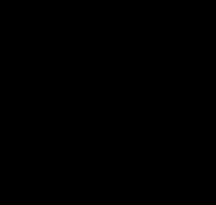
\includegraphics[scale=1.0]{./gw/greenpoles.pdf}
\end{center}
\caption{\small \label{fig:greenpoles} Pole structure 
of the Green's function. 
The occupied electronic states are
slightly above the real frequency axis and below the chemical 
potential $\mu$, the unoccupied states are located above the Fermi
level and slightly below the real axis. The poles of the Green's 
function correspond to the addition/removal energies 
in the system. This example is for a system with a discrete series of 
excitations and an energy gap between occupied and unoccupied states
of $E_{g}$.}
\end{figure}
%
To demonstrate this it is necessary to Fourier transform the Green's from the time
domain to the frequency domain. This can be accomplished by 
rewriting the field operators in the Heisenberg representation:
%
\begin{equation}
\label{eq:heisenop}
\cfield(\r,t) = e^{i\hat{H}t}\cfield(\r) e^{-i\hat{H}t}.
\end{equation}
%
We then introduce a complete set of states which describe all the possible 
intermediate excitations of the system to $N'$ particles 
and their $s$ excited states,~$|N',s\ket$:
%
\begin{equation}
\label{eq:compstates}
\sum_{s}|N', s\ket \bra N',s| = \I,
\end{equation}
%
where $\I$ is the identity matrix.
We also note that:
%
\begin{equation}
H|N,s\ket = E^{s}_{N}|N,s\ket.
\end{equation}
%
%
If one inserts Eqs. \ref{eq:heisenop} and \ref{eq:compstates} into Eq.~\ref{eq:green} it is possible 
to write the Green's function in the time domain as:
%
\begin{align}
\label{eq:grtimedom}
G(\r,t,\rp,t') & = & \sum_{s} -i\Theta(t-t') e^{i(E^{0}_{N} - E_{N'}^{s})(t-t')}\bra N|\field(\r)|N',s\ket\bra N',s|\cfield(\r')|N\ket \nonumber \\
	  &+ & \sum_{s} i\Theta(t'-t) e^{-i(E_{N}^{0} - E^{s}_{N'})(t-t')}\bra N|\cfield(\r') |N',s\ket \bra N',s|\field(\r)| N \ket.
\end{align}
%
Now Eq.~\ref{eq:grtimedom} gives the Green's function in the time domain and the arguments depend 
only on differences in time $t-t'$. By introducing the time variable $\tau = t-t'$ it is 
straightforward to define a Fourier transform:
%
\begin{equation}
G(\r,\r';\omega) = \frac{1}{2\pi} \int_{-\infty}^{\infty} G(\r,\r,\tau) e^{i\omega\tau} d\tau,
\end{equation}
%
and represent the Green's function in the frequency domain:
%
\begin{eqnarray}
\label{eq:greenfreq}
G(\r,\rp;\omega) & = &\sum_{s} \frac{\bra N|\field(\r) |N',s\ket \bra N',s|\cfield(\r')| N \ket}{\omega - (E^{s}_{N'} - E^{0}_{N}) + i\delta} \nonumber \\
	  		   & - & \sum_{s}\frac{\bra N|\cfield(\r') |N',s\ket \bra N',s|\field(\r)| N \ket}{\omega + (E^{s}_{N'} - E^{0}_{N}) - i\delta}.
\end{eqnarray}
%
The infinitesimal factors of $i\delta$ ensure that the Fourier 
transform converges at infinite time arguments.
The presence of the field operators implies that the only 
non-zero contributions to Eq.~\ref{eq:greenfreq} are between 
the ground and excited states of the $N'=N+1$ and the $N'=N-1$ systems. 
Therefore it is convenient to make the follow substitution~\cite{inkson}:
%
\begin{equation}
(E^{s}_{N+1} - E^{0}_{N}) = \epsilon^{s}_{N+1},
\end{equation}
%
with a similar expression for the $N-1$ system. The variable $\epsilon^{s}_{N\pm1}$ 
is the energy difference of an excited state in the $N\pm1$ many body system and 
the ground state of the $N\pm1$ system. 
This leads us to:
%
\begin{eqnarray}
\label{eq:greenpoles}
G(\r,\rp;\omega) = \sum_{s} \frac{\bra N|\field(\r) |N+1,s\ket \bra N+1,s|\cfield(\r')| N \ket}{\omega - \epsilon^{s}_{N+1} + i\delta} \nonumber \\
			 		-\sum_{s} \frac{\bra N|\cfield(\r')|N-1,s\ket \bra N-1,s|\field(\r)| N \ket}{\omega + \epsilon^{s}_{N-1} - i\delta}.
\end{eqnarray}
%
The poles of Eq.~\ref{eq:greenpoles} are represented schematically in Fig.~\ref{fig:greenpoles} 
and correspond to the energies of the excitations from $N$ to $N\pm1$ electrons 
in an interacting many body system. Having discussed the pole structure of 
the Green's function we now proceed to define the equation of motion.

\section{Green's function methods}
\noindent
Lars Hedin first developed the $GW$ approximation with
his publication ``New Method for Calculating the One-Particle Green's Function
with Application to the Electron-Gas Problem.''~\cite{hedin65}. In this work Hedin developed a
self-consistent system of equations for including all the interaction effects
in a many electron system. Hedin describes the
connection between his work and the development of Green's
functions methods by Schwinger in Ref.~\cite{schwinger51} 
working in the field of quantum electrodynamics.
An early review of the applications of Green's function methods and
Feynman diagrams to the many electron problem was given in Ref.~\cite{pratt63}. The procedure
has been extensively studied in the 
intervening thirty years and Refs.~\cite{aulbur00, aryasetgunnarsson98, onida02}
provide a review of the contemporary state of the field.
%
\subsection{Equation of motion}
\noindent
To derive the equation of motion for the Green's 
function we need the time derivative of Eq.~\ref{eq:green}. 
This derivative in turn requires working out the time 
dependence of the field operators appearing in Eq.~\ref{eq:green}:
%
\begin{equation}
\frac{\partial \field(\r,t)}{\partial t} = i[\hat{H},\field(\r,t)].
\end{equation}
%
The time dependence of the field operator is determined by the 
commutator between the Hamiltonian and the field operator.
%
The general Hamiltonian we will consider can be separated into two parts:
%
\begin{equation}
\H =  \H_{0} + v(\r,\r')\delta(t-t'),
\end{equation}
%
where the $\H_{0}$ term describes the kinetic energy of the electron and the interaction of the 
electron with an ionic lattice. 
The $v(\r,\r')\delta(t-t')$ term represents the inter-electron Coulomb repulsion.
We differentiate Eq.~\ref{eq:green} with respect to time to arrive at the following result:
%
\begin{align}
\label{eq:greqmotn}
\left[i\frac{\partial}{\partial t} - \H_{0}\right]G(\r,\r',t,t') +  & &  \nonumber \\
i\int v(\r,\r'')\bra N| T[\cfield(\r'',t)\field(\r'',t)\field(\r,t)\cfield(\rp,t')] |N \ket d\r'' & = & \delta(\r-\rp)\delta(t-t').
\end{align}
%
The right hand side of Eq.~\ref{eq:greqmotn} comes immediately from 
the fact that $\frac{\partial}{\partial t}\Theta(t-t') =\delta(t-t')$, 
and the anti-commutator identity for fermionic field operators. 
%
The commutator for the single particle operator, $\H_{0}$, and the 
field operator can be separated directly. 
The final term under the integral sign results from the commutator
involving the field operators and the Coulomb interaction.

The number of indices that we require to keep track of everything when 
describing multi-particle propagators, and, in the next section, 
when taking functional derivatives, can be very large. 
Therefore, in order to proceed, we will employ the compressed notation for space, 
time, and spin: $1 = (\r,t,\sigma)$, $2=(\r',t',\sigma')$, and so on.

The quantity under the integral sign in Eq.~\ref{eq:greqmotn} is a two particle Green's function:
%
\begin{equation}
\label{eq:2pgreenfxn}
G_{2}(1,2,3,4) = \frac{1}{i^{2}} \bra N|T[\cfield(4)\cfield(3)\field(2)\field(1)]|N\ket.
\end{equation}
%
Eq.~\ref{eq:greqmotn} expresses the single particle Green's function now defined 
implicitly in terms of the two particle Green's function. The two particles Green's function is 
defined in terms of  four field operators. The equation of motion for the two particle Green's 
function would then involve terms with an increasing number of field operators due to the coupling 
via the Coulomb interaction.
This is the heart of the many body problem: an infinite expansion of interaction terms,
all of comparable magnitude, due to the strength of the Coulomb coupling.

When trying to solve equations of the form Eq.~\ref{eq:greqmotn} it is convenient to 
replace the function appearing under the integral sign with a new function,
termed a kernel, and then attempt to solve the system of equations in terms of this kernel.
In order to solve Eq.~\ref{eq:greqmotn} and derive the $GW$ approximation,
we will introduce three new quantities: $\Sigma$, $P$ and $\Gamma$.
Respectively these are named the self-energy, the polarization propagator, and the vertex function.
At this stage we introduce the self-energy $\Sigma$, by rewriting the integrand in Eq.~\ref{eq:greqmotn} as:
%
\begin{equation}
\label{eq:greqmsig}
\left[i\frac{\partial}{\partial t} - \H_{0}\right]G(\r,\r',t,t') - \int \Sigma(\r,\r'',t,t'')G(\r'',\rp,t'',t')d\r''dt'' =  \delta(\r-\rp)\delta(t-t').
\end{equation}
%
The equation now has the shape that we discussed in Sec.~\ref{sec:thelda} when discussing
the generalized Kohn-Sham exchange correlation potential. The Green's 
function evolves under the single particle
interactions included in $\H_{0}$ and according to some non-local, energy dependent potential, $\Sigma$.
What remains to be done is to show how we can calculate $\Sigma$ efficiently, and remove the 
implicit definition of the Green's function in terms of multi-particle propagators.

\subsection{Functional derivative of the Green's function}
\noindent
Eq.~\ref{eq:greqmotn} defines the equation of motion for the one particle Green's
function by making reference to the two particle Green's function.
In the following we will rewrite the equation of motion so that it is entirely defined in
terms of the single particle Green's function. This can be
accomplished by relating the single particle Green's function to the two particle Green's
function via a functional derivative.

To derive Hedin's equation we make some formal modifications. The following derivation follows closely
that presented in Appendix A of Ref.~\cite{hedin65}, the review article of \cite{strinati88} 
and the textbook of Inkson \cite{inkson}. A few important functional identities 
are reproduced in Appendix~\ref{app:funcdiv}. These are required to manipulate the equations 
and obtain their final closed form.

First Eq.~\ref{eq:greqmotn} is rewritten to include a perturbing potential $\phi(1)$:\footnote{For our
purposes a local scalar potential $\phi(1)$ is sufficient to derive the $GW$ approximation. More general 
perturbations, e.g. coupling to non-local vector potentials, are developed in Ref.~\cite{strinati88}.}
%
\begin{align}
\label{eq:greqmotn2}
\left[i\frac{\partial}{\partial t} - \H_{0} - \phi(1)\right]G(1,2) +& \nonumber \\
i\int v(1,3)\delta(t_{3}-t_{1})\bra N| T[\cfield(3)\field(3)\field(1)\cfield(2)] |N \ket d3 &= \delta(1,2).
\end{align}
%
The perturbing potential will be set to zero at the end of the derivation.

Eq.~\ref{eq:greqmotn2} allows us to separate motion generated by the original Hamiltonian, 
which is composed of the single electron and electron-electron
interaction terms, from the time development due to the perturbation $\phi(1)$. The perturbing potential 
allows us to define the functional derivative of the system's Green's
function, and hence relate the propagation of a single particle to the propagation of multiple particles. 
The introduction of $\phi(1)$ allows us to generate an infinite series of terms 
describing the electron-electron interactions in terms of functional derivatives.

Eq.~\ref{eq:greqmotn2} is rewritten so that the field operators refer to the ground-state field
operators, denoted $\field_{0}$, and their time development due to $\phi(1)$ is made explicit:
%
\begin{equation}
\label{eq:intergr}
G(1,2) =  \frac{\bra N|\hat{T}[\hat{S}\field_{0}(1)\cfield_{0}(2)]|N\ket}{\bra N| \hat{S} |N\ket}.
\end{equation}
%
The $\hat{S}$ operator propagates the ground-state field operators according to:
%
\begin{equation}
\hat{S} = T\rm{exp}\left[-i\int_{t_{1}}^{t_{2}} \phi(2)\field_{0}(2)\cfield_{0}(2)d{2}\right].
\end{equation}
%
This separation ensures the time development of the field operators due to $\phi$ is made explicit
and the field operators have no implicit dependence on the perturbation. In this way the field 
operators reflect only the dynamics of the underlying electron system interacting via the Coulomb interaction.

By functional differentiation of Eq.~\ref{eq:intergr} with respect to the perturbing potential $\phi$ 
the two particle Green's function can be written:
%
\begin{equation}
\label{eq:funcdifgr}
G(1,3,2,3^{+}) = G(1,2)G(3,3^{+}) - \frac{\delta G(1,2)}{\delta \phi(3)}.
\end{equation}
%
To arrive at Eq.~\ref{eq:funcdifgr} we used the quotient rule as it applies to functional derivatives, 
and that the variation in $S$ is:   
%
\begin{equation}
\frac{\delta \hat{S}}{\delta\phi(3)} = i \hat{S} \field(3)\cfield(3).
\end{equation}
%
We can now use Eq.~\ref{eq:funcdifgr} to replace the two particle propagator in Eq.~\ref{eq:greqmotn}:
%
\begin{align}
\label{eq:greqmwfd}
\left[i\frac{\partial}{\partial t}-\H_{0}(1)-V(1)\right]G(1,2) &
	-i\int v(1,3)\frac{\delta G(1,2)}{\phi(3)}d3 &=\delta(1,2),
\end{align}
%
where: 
%
\begin{equation}
V(1) = \phi(1) - i\int v(1,3) G(3,3^{+})d3.
\end{equation}
%
Eq.~\ref{eq:greqmwfd} has now separated into two terms. The first term
contains the single electron components
of the Hamiltonian, the perturbing potential, and what can now be
identified as the Hartree potential, i.e. the mean field
felt by an electron due to the classical potential generated from the electron cloud 
discussed in Section~\ref{sec:hohnkohn}. The connection can be seen directly 
by noting that the quantity $G(3,3^{+})$ is just the electronic density. 
\footnote{It is important to see this connection: the diagonal elements 
of the Green's function are just the electron density. 
The superscript $+$ is added to avoid problems
with the definition of the step function in the time 
domain when $(t-t')=0$.}

The second term contains the \emph{bare} Coulomb interaction 
multiplied by the functional derivative of the 
one particle Green's function. Upon comparison of 
Eq.~\ref{eq:greqmwfd} with Eq.~\ref{eq:greqmsig} we can 
rearrange terms by observing:
%
\begin{equation}
\int \Sigma(1,3)G(3,2)d3 = -i\int v(1,3) \frac{\delta G(1,2)}{\delta \phi(3)}d3,
\end{equation}
%
or by isolating the self-energy $\Sigma$ as: %(where we have used app. 1 Eq.~\ref{eq:expansionrule}):
%
\begin{equation}
\label{eq:sigma}
\Sigma(1,2) = i \int v(1,4) G(1,3) \frac{\delta G^{-1}(4,2)}{\delta\phi(4)}d3d4.
\end{equation}
%
We now retrieve the equation of motion for the Green's function 
as it appeared in Eq.~\ref{eq:greqmsig} as:
%
\begin{equation}
\label{eq:greqmsig2}
\left[i\frac{\partial}{\partial t} - \H_{0}(1) - V(1)\right]G(1,2) - i\int \Sigma(1,3)G(3,2)d3 = \delta(1,2).
\end{equation}
%
One could formally solve this equation as it stands using an iterative method, 
however it is worth noting that the resulting expansion of the self-energy $\Sigma$ 
would contain increasing powers of the bare Coulomb interaction $v$. 
It is unlikely that the resulting series will converge particularly 
quickly, if it converges at all. 
%
Therefore it is necessary to expand $\Sigma$ in a closed form without making 
reference to the perturbing potential $\phi$. In doing so the equations are rearranged so that
the bare Coulomb interaction is modified and the electrons experience 
an effective screened Coulomb interaction. In a classical picture the electrons will interact
via a Coulomb interaction screened by the system's dielectric function. 
This will be done in the next two sections.
%
\section{Hedin's equations}
\subsection{Dielectric function}
\label{sec:dielecfun}
\noindent
At this point it is useful to introduce the following functional relationships 
which define the dielectric function in a many-body system.
We will switch back to labeling time and space coordinates as $\r,t$ 
here for ease of reference Section~\ref{sec:nscfstern}. 

The effective potential acting on the electrons is:
%
\begin{equation}
\label{eq:internalpot}
V(\r,t) = \phi(\r,t) - i\int v(\r,\r') G(\r',\r',t,t^{+}) d\r',
\end{equation}
%
where $iG(\r',\r',t,t^{+})$ is the single particle density $n(\r')$.
%
We now define the inverse dielectric function to be the self-consistent variation 
of this effective potential with respect to the external perturbing potential:
%
\begin{equation}
\label{eq:invepsvphi}
\inveps(\r,t,\r',t') = \frac{\delta V(\r,t)}{\delta\phi(\r',t')}.
\end{equation}
%
Upon inserting Eq.~\ref{eq:internalpot} into Eq.~\ref{eq:invepsvphi} we arrive at:
%
\begin{equation}
\label{eq:simpphys}
\inveps(\r,t,\r',t') = \delta(\r-\r')\delta(t-t') + \int v(\r,\r'') \frac{\delta n(\r'',t)}{\delta\phi(\rp,t')}d\r''.
\end{equation}
%
Eq.~\ref{eq:simpphys} has a simple physical interpretation. The inverse dielectric function 
encodes the self-consistent variation in the charge density 
with respect to a variation in the potential $\phi$.
This rearrangement of charge means that the bare Coulomb interaction
 between two points is altered by the induced screening in
the interacting medium. This altered Coulomb interaction is the 
screened Coulomb interaction, and can be defined 
in terms of the inverse dielectric function as:
%
\begin{equation}
\label{eq:scrncoul}
W(\r,t,\r',t') = \int v(\r,\r'')\delta(t-t'') \frac{\delta V(\r',t')}{\delta \phi(\r'',t'')} dr''dt''.
\end{equation}
%
The screened Coulomb interaction can also be written as an integral equation: 
%
\begin{equation}
\label{eq:dysw}
W(\r,t,\r',t') =  v(\r,\r') + \int d\r''' v(\r,\r''')\int P(\r''',t,\r'',t'') W(\r'',t'',\r',t')dt''d\r''.
\end{equation}
%
where the polarizability, $P$, has been introduced:
%
\begin{equation}
P(\r,\r',t,t') = \frac{\delta n(\r',t')}{\delta V(\r,t)}.
\end{equation}
%
Alternatively we can introduce the dielectric function in its non-inverted form as:
%
\begin{equation}
\label{eq:epschap2}
\epsilon(\r,t,\rp,t') = \delta(\r-\r')\delta(t-t') - \int v(\r,\r'') P(\r'',t'',\r',t') \delta(t-t'') d\r''dt''.
\end{equation}

\subsection{Hedin's equations}
\noindent
While the Coulomb repulsion between electrons remains the bare Coulomb interaction, 
the dielectric function provides a route to interpreting 
an auxiliary system of electrons interacting via a \emph{screened} Coulomb interaction.

In order to include this screening implicitly in the definition of the self-energy, we 
go back to the definition of $\Sigma$ in Eq.~\ref{eq:sigma}. We now use the chain 
rule to take the functional derivative of $G$ with 
respect to the total potential $V$ rather than the perturbing potential $\phi$:
%
\begin{equation}
\label{eq:funcdifsig}
\Sigma(1,2) =  i\int v(1,4) G(1,3)\frac{\delta G^{-1}(3,2)}{\delta V(5)}\frac{\delta V(5)}{\delta\phi(4)}d3d4d5.
\end{equation}
%
By comparison of Eqs. \ref{eq:invepsvphi}, \ref{eq:scrncoul}, and \ref{eq:funcdifsig} we can combine
the inverse dielectric function and the bare Coulomb interaction into the screened Coulomb interaction $W$:
%
\begin{equation}
\Sigma(1,2) =  i\int W(1,4)G(1,3)\frac{\delta G^{-1}(3,2)}{\delta V(4)}d3d4.
\end{equation}
%
The final piece of notation to be introduced is the vertex function. This is defined as the variation 
of the inverse Green's function with respect to the potential $V$:
%
\begin{equation}
\label{eq:vertex}
\Gamma(1,2;3) = \frac{\delta G^{-1}(1,2)}{\delta V(3)}.
\end{equation}
%
Having obtained the expression for the vertex function in Eq.~\ref{eq:vertex} we
can write all of Hedin's equations in a closed form.
We summarize Hedin's equations describing the interacting Green's function,
the screened Coulomb interaction, the polarizability, and the vertex function of the system:
%
\begin{align}
\label{eq:hedinsig}
&\Sigma(1,2)   = i\int W(1^{+},4)G(1,3)\Gamma(3,2;4)d4d3 &   \\
\label{eq:hedinw}
&W(1,2)        =  \int \inveps(1,3)v(3,2) d3 &               \\
\label{eq:hedineps}
&\epsilon(1,2) =  \delta(1,2) - \int v(1,3)P(3,2)d3 &        \\
\label{eq:hedinpol}
&P(1,2)        = -i\int G(1,3)\Gamma(3,4;2) G(4,1^{+})d4d3 & \\
\label{eq:hedinvert}
&\Gamma(1,2;3) = \delta(1,2)\delta(1,3) + \int \frac{\delta\Sigma(1,2)}{\delta G(4,5)}G(4,6)G(7,5) \Gamma(6,7;3)d4d5d6d7 & 
\end{align}

In summary, we started from the equation of motion. Then a relationship between
the two particle Green's function and the one particle Green's function was found.
This relationship takes the form of a functional derivative of the one particle Green's function with
respect to a perturbing potential. When everythin is written in terms 
of the one particle Green's function we have obtained a set of equations 
that need to be solved self-consistently. 
These are known as Hedin's equations. When solved iteratively these 
equations incorporate all the many body effects of a many-electron system.

\section{$G_0W_0$ self-energy and corrections to LDA eigenvalues}
\noindent
In the first section of this chapter we have discussed the
procedure for constructing the $G_0W_0$ self-energy operator.
We have also discussed some of the considerations required when
performing DFT calculations within a planewaves basis set.
It remains to show how the $G_0W_0$ self-energy can be
used to connect the eigenvalues obtained from a DFT calculation.

We proceed as in Ref.~\cite{HL86} by assuming the $G_0W_0$
self-energy can be treated as a perturbation to the
DFT Kohn-Sham exchange and correlation potential.

In Chapter~\ref{chap:dftgw} we discussed the quasiparticle equation:
%
\begin{equation}
\label{eq:qpeq2}
\left[-\frac{1}{2}\nabla^{2} + \hat{V}^{\rm{ion}} + \hat{V}^{\rm{H}}\right]\phi_{n\k}(\r) + \int{d}\r' \Sigma(\r,\r';E_{n\k})\phi_{n\k}(\r')=E_{n\k}\phi_{n\k}(\r).
\end{equation}
%
By adding and subtracting $V_{xc}(\r)\psi_{n\k}(\r)$ one obtains:
%
\begin{equation}
(-\frac{1}{2}\nabla^{2} + \hat{V}^{\rm{ion}} + \hat{V}^{\rm{H}} + \hat{V}^{\rm{xc}})\phi_{n\k}(\r) + \int{d}\r' \left[\Sigma(\r,\r';E_{n\k})-\hat{V}^{\rm{xc}}(\r')\delta(\r,\r')\right]\phi_{n\k}(\r') = E_{n\k}\phi_{n\k}(\r).
\end{equation}
%
If we treat $\Sigma-V^{\rm{xc}}$ as a perturbation we can express $E_{n\k}$
in terms of the Kohn-Sham eigenvalues $\epsilon^{\rm{LDA}}_{n\k}$ using 
first order perturbation theory:
%
\begin{equation}
\label{eq:QPenergy}
E_{n\k}^{\rm{QP}} = \epsilon_{n\k}^{\rm{LDA}} + \bra n\k| \Sigma(E_{n\k}^{\rm{QP}}) - \hat{V}^{\rm{xc}}|n\k\ket.
\end{equation}
%
Following Ref.~\cite{HL86} we expand the self-energy operator to first order around the LDA eigenvalue:
%
\begin{equation}
\label{eq:sigmafirst}
\Sigma( E_{nk}^{\rm{QP}} ) = \Sigma(\epsilon_{nk}^{\rm{LDA}}) + \frac{\partial\Sigma(\omega)}{\partial \omega}\bigg|_{\omega = \epsilon_{n\k}^{\rm{LDA}}}(E_{n\k}^{\rm{QP}} - \epsilon_{n\k}^{\rm{LDA}}). 
\end{equation}
%
The quasiparticle energy can than be obtained by substituting Eq.~\ref{eq:sigmafirst} into Eq.~\ref{eq:QPenergy}:
%
\begin{equation}
\label{eq:QPfirst}
E_{n\k}^{\rm{QP}} = \epsilon_{n\k}^{\rm{LDA}} + \left(1-\frac{\partial\Sigma(\omega)}{\partial \omega}\bigg|_{\omega=\epsilon_{n\k}^{\rm{LDA}}}\right)^{-1}(E_{n\k}^{\rm{QP}} - \epsilon_{n\k}^{\rm{LDA}}). 
\end{equation}
%
The quasiparticle renormalization value $Z$ is defined by:
%
\begin{equation}
Z_{n\k} =  \left[1-\frac{\partial\Sigma(\omega)}{\partial \omega}\bigg|_{\omega = \epsilon_{n\k}^{\rm{LDA}}}\right]^{-1}.
\end{equation}
%
In summary, we find the expression for the $G_{0}W_{0}$ perturbative correction to the LDA eigenvalues is:
%
\begin{equation}
\label{eq:qpcorrpert}
E^{\rm{QP}}_{n\k} =  \epsilon^{\rm{LDA}}_{n\k} + Z_{n\k}\bra n\k|\Sigma(\epsilon^{\rm{LDA}}_{n\k})-V^{xc}_{n\k}| n\k\ket.
\end{equation}
%

\section{The Spectral function}
\subsection{The $GW$ spectral function}
\label{sec:spec}
\noindent
In this section we introduce the spectral function. For simplicity we will contract the
Bl\"och notation $n\k$ to a single index $n$, and then reintroduce the full Bl\"och notation when
we arrive at the final expression for the spectral function.

Given a set of single particle eigenvectors $\phi_{m}(\r)$ we can take matrix elements of the
single particle states with the Green's function and self-energy:
%
\begin{eqnarray}
G_{mn}(\omega)       = \int \int \phi_{m}^{\star}(\r) G(\r,\r';\omega) \phi_{n}(\r')  d\r d\r', \\
\Sigma_{mn}(\omega)  = \int \int \phi_{m}^{\star}(\r) \Sigma(\r,\r';\omega) \phi_{n}(\r') d\r d\r'.
\end{eqnarray}
%
We can employ the same notation for matrix elements with $V^{\rm{xc}}(\r)$,
and the Kohn-Sham Hamiltonian $\hat{H}^{\rm{KS}}$.
%
In matrix notation the Dyson equation \cite{inkson} can be written:
%
\begin{equation}
\label{eq:matdys}
G^{-1} = G_{0}^{-1} - [\Sigma(\omega) - V_{\rm{xc}}].
\end{equation}
%
Eq. \ref{eq:matdys} gives the expression for interacting Green's function.
We note that the exchange and correlation potential of the ground state
calculation is subtracted from the final self-energy. If the Green's function is diagonal
in the state indices we can invert each element of the matrix and write:
%
\begin{equation}
G_{nn}(\omega) = \frac{1}{\omega -\epsilon^{\rm{KS}}_{n}+{\rm Re}\Sigma_{nn}(\omega)-V^{\rm{xc}}_{nn}+{\rm Im}\Sigma_{nn}(\omega)}.
\end{equation}
%
In the case where the non-diagonal elements cannot be ignored,
a full matrix inversion would be required to construct the Green's function:
%
\begin{equation}
G_{mn}(\omega) = [\omega \delta_{mn} - \epsilon^{\rm{KS}}_{mn}\delta_{mn} + {\rm Re}\Sigma_{mn}(\omega) - V^{\rm{xc}}_{nn} + {\rm Im}\Sigma_{mn}(\omega)]^{-1}.
\end{equation}

We can employ the same notation for matrix elements with $V^{\rm{xc}}(\r)$,
and the Kohn-Sham Hamiltonian $\hat{H}^{\rm{KS}}$.
%
In matrix notation the Dyson equation \cite{inkson} can be written:
%
\begin{equation}
\label{eq:matdys}
G^{-1} = G_{0}^{-1} - [\Sigma(\omega) - V_{\rm{xc}}].
\end{equation}
%
Eq. \ref{eq:matdys} gives the expression for interacting Green's function.
We note that the exchange and correlation potential of the ground state
calculation is subtracted from the final self-energy. If the Green's function is diagonal
in the state indices we can invert each element of the matrix and write:
%
\begin{equation}
G_{nn}(\omega) = \frac{1}{\omega -\epsilon^{\rm{KS}}_{n}+{\rm Re}\Sigma_{nn}(\omega)-V^{\rm{xc}}_{nn}+{\rm Im}\Sigma_{nn}(\omega)}.
\end{equation}
%
In the case where the non-diagonal elements cannot be ignored,
a full matrix inversion would be required to construct the Green's function:
%
\begin{equation}
G_{mn}(\omega) = [\omega \delta_{mn} - \epsilon^{\rm{KS}}_{mn}\delta_{mn} + {\rm Re}\Sigma_{mn}(\omega) - V^{\rm{xc}}_{nn} + {\rm Im}\Sigma_{mn}(\omega)]^{-1}.
\end{equation}

At this stage we introduce the spectral function by defining it in terms of the Green's function:
%
\begin{equation}
A_{mn}(\omega) = {\rm Im} |G_{mn}(\omega)|.
\end{equation}
%
Reintroducing the Bloch notation we can write the full spectral function
for the diagonal Green's function:
%
\begin{equation}
\label{eq:aspec}
A_\k(\omega) = \frac{1}{\pi}\sum_{n} \frac{|{\rm Im}\Sigma_{n\k}(\omega)|}
{[\omega- \epsilon_{n\k}-({\rm Re}\Sigma_{n\k}(\omega) -V^{\rm{xc}}_{n\k})]^{2} + \left[{\rm Im}\Sigma_{n\k}(\omega)\right]^{2}}.
\end{equation}

The spectral function helps clarify the quasiparticle picture. Eq.~\ref{eq:aspec} is strongly
peaked when the frequency $\omega$ sweeps through the renormalized
eigenvalue $\epsilon_{n\k} + {\rm Re}(\Sigma_{n\k}(\omega) - V^{\rm{xc}}_{n\k}) $. Given
the frequency dependence of $\Sigma$ additional zeros in the real part of the
denominator of Eq. \ref{eq:aspec} are possible. These can correspond to the
appearance of new excitations which are not present in the non-interacting system. Finally
the imaginary part of the self-energy introduces a broadening of the the quasiparticle peak
and is associated with lifetime effects.

\subsection{Contact with experiment}
\noindent
Angle Resolved Photoemission Spectroscopy (ARPES) is a very useful
probe for investigating the electronic structure of materials~\cite{damascelli04}.
%Incident radiation on a sample can excite electrons via the photoelectric effect. 
%These excited electrons can then propagate to a detector where their energy and momentum 
%is measured. Given the momentum and energy of the impinging light source it is 
%possible to determine the initial electronic state the captured electron occupied 
%in the material. 
%
The intensity of the electrons captured at the experimental detector, $I_{\k}(\omega)$,
can be expressed in terms of the quasiparticle spectral function~\cite{damascelli04}:
%
\begin{equation}
\label{eq:photoemission}
I_{\k}(\omega) = I_{0}(\k,\nu)f(\omega)A_{\k}(\omega),
\end{equation}
%
Where $\nu$ is the frequency of the incident radiation and $f(\omega)$ is the Fermi-Dirac distribution.
The factor $I_{0}(\k,\nu)$ includes matrix element effects, i.e.
the strength of the coupling of the initial and final electron states via
the electromagnetic probe, the effect of surfaces, and 
inelastic scattering in the sample~\cite{damascelli04}.

\subsection{Bardyszewski-Hedin theory of photoemission}
\noindent
A comprehensive analysis of the connection between the spectral function
and photoemission data is given by Bardyszewski and Hedin in Ref.~\cite{bardy85}.
Their formulation begins by relating the photocurrent, $J$, i.e. the number
of electrons ejected from the sample, per unit solid angle and energy
to the intensity, $I$, measured at the detector:
%
\begin{equation}
\frac{\partial^{2}J}{\partial \Omega \partial \epsilon_{\k}} \sim I.
\end{equation}
%
The standard definition for the intensity is then given in Refs.~\cite{goldberger64, almbladh83}:
%
\begin{equation}
\label{eq:intens}
I = \sum_{s}|\bra \k,N-1,s|\hat{\Delta}|N\ket|^{2}\delta(\epsilon_{\k}-\epsilon_{s}-\omega).
\end{equation}
%
The $|\k,N-1,s\ket$ state is a product state of the photoelectron with wave vector
$\k$ and the $|N-1, s\ket$ many electron wavefunction described in Eq. \ref{eq:compstates}.
The frequency of the incoming radiation is $\omega$. The $\hat{\Delta}$
operator is the electric dipole operator.

Eq.~\ref{eq:intens} explicitly couples many-body states via the dipole operator.
The intrinsic contribution of a particular photoelectron $\tilde{\phi}_{\k}$, to the measured photocurrent
can now be written in terms of the one-electron spectral
function discussed in Section~\ref{sec:spec}~\cite{bardy85}:
%
\begin{equation}
\label{eq:barhed}
I(\k,\omega)=\int \tilde{\phi}^{\star}_{\k}(\r)\hat{\Delta}(\r)A(\r,\r';\epsilon_\k-\omega)\hat{\Delta}(\r')\tilde{\phi}_{\k}(\r')d\r d\r'.
\end{equation}
%
If we assume the spectral function is diagonal in $\r$, $\r'$, and exploit the matrix
notation for the spectral function from the previous section we arrive at the expression:
%
\begin{equation}
I(\k,\omega) \approx \sum_{n} |\bra\tilde{\phi}_{\k}|\hat{\Delta}|\phi_{n}\ket|^{2} A_{nn}(\epsilon_{\k}-\epsilon_{n}-\omega).
\end{equation}
%
The photoelectron will not generally travel unimpeded to the detector. 
Along the way the photoelectron can scatter off of phonons, plasmons, 
or other particle-hole excitations.
Ref. \cite{bardy85} provides a detailed derivation of the 
expressions reported here for the intrinsic intensity
of the photocurrent and the possible types of quasiparticle 
excitations in an interacting system.
These results are mentioned here because they provide a direct 
connection between experimental probes and the mathematical 
formalism of the $GW$ approximation.

\section{Alternative Functionals and Tight Binding}
Armed with the local density approximation, a computer, 
and the comfort of a well defined variational principle
means computational material scientists are in a position 
to go out and do a significant amound of damage. In 
this section it is useful to look at a few different functional
forms.

The first constraint we have is $\int\rho(\r)d^{3}\r = N$ incorporating this
constraing using a Lagrange multiplier technique with the fact that we want
to find a variational minimum for the energy we can write:
%
\begin{equation}
\frac{\delta}{\delta \rho} \left[E[\rho] - \mu(\int \rho(\r)d\r - N)\right] = 0,
\end{equation}
%
which leads to:
%
\begin{equation}
\frac{\delta E[\rho]}{\delta \rho}= \mu.
\end{equation}

\section{Purely Functional Forms}
Finnis' textbook gives a comprehensive discussion of functionals,
the Hohenberg-Kohn Functional and the Harris-Foulkes functional.
His development is far more thorough than what is discussed here. 
The important connections to make in the present collection
is that we can point out a direct connection between the

\begin{itemize}
\item A direct relation between the second nd order variation in $E_{\rm xc}$ and the dielectric function can be made.
\item We can define the Generalized Harris-Foulkes Functional which will clarify our ideas about optimizing the computed
      electron densities and changing the potentials we are asking the electrons to move in.
\end{itemize}

The first point means we can connect the exchange-correlation functional, 
which is mysterious and foreign, to a dielectric function, which has a pleasing 
classical picture and is familiar.

The second point is essential because it will justify the use of certain 
computational approaches and clarify why, in some cases, a single shot GW
calculation might ``work", and where it might not. The Generalized Harris-Foulkes
and quantify what is meant by an optimum model of our system and allow for the
construction of densities and potentials that reach this optimum position in 
the functional space. 

The text of this section will be kept to a minimum. It should be viewed as a
useful collection of functional definitions all contained in one place. 
The Hohenberg-Kohn-Sham Energy written in its pure functional form,
as a set of non-interacting electrons, expanded to first order, expanded to
second order, and the Harris-Foulkes function are all discussed.

\subsection{HKS}
\begin{equation}
\label{eq:hks}
E^{\rm HKS} = T[\rho] + E_{\rm H}[\rho] + E_{\rm xc}[\rho] + E_{\rm eZ}[\rho] + E_{\rm ZZ}
\end{equation}

Taking the variation of Eq.~\ref{eq:hks} with respect to the density gives:
%
\begin{equation}
\frac{\delta E^{\rm HKS}}{\delta \rho} = \frac{\delta T[\rho]}{\delta \rho} + V_{\rm H}[\r] + V_{\rm xc}[\r] + V_{\rm ext}[\r] = \mu
\end{equation}
%
where $V_{xc} = \frac{\delta E_{xc}[\rho]}{\delta \rho}$.

In the local density approximation:
%
\begin{equation}
E_{\rm xc}[\rho] = \int\epsilon^{xc}[\rho(\r)]\rho(\r)dr
\end{equation}
%
with epsilon taking its value for the homogeneous electron gas at 
every point. As a potential the chain rule needs to be used to obtain:
%
\begin{equation}
\frac{\delta E_{\rm xc}[\rho(\r)]}{\delta \rho(\r)} = \epsilon^{xc}(\r) + \frac{d \epsilon^{xc}[\rho(\r)]}{d\rho}|_{\rho(\r)}\rho(\r)
\end{equation}
%

If the Kohn-Sham trick of introducing a set of non-interacting electrons is used the Energy can be written
%
\begin{equation}
E^{\rm HKS}[\rho] = \sum_{i}f_{i}\bra \psi_{i}|\hat{T} + \hat{V}_{\rm eff}|\psi_{i}\ket - \frac{1}{2}\int\rho V_{\rm H} - \int\rho V_{xc} + E_{xc}[\rho] + E_{ZZ}
\end{equation}

\subsection{Harris Fragments}
Harris's approach \cite{harris85} comes from the perspective of bringing together 
"interacting fragments" \footnote{The idea had been treated in K. Nikulin, Zh. Tekhn. Fiz. XLI, 41 (1971) 
[Sov. Phys. — Techn. Phys. 16, 28 (1971)]; R. G. Gordon and Y. S. Kim, J. Chem. Phys. 56,3122 (1972)
see also Wendel and Martin \cite{wenel79}. }
Two separate fragments for which we can obtain the density are brought together. 
The new effective potential is generated from the sum of the fragment's densities, 
and the single particle eigenvalues are recomputed.

The idea is quite intuitive. We take a slab of one thing $n_{1}(x)$ 
and a slab of another thing $n_{2}(x)$ and form the combined density 
$n_{f}= n_1 + n_2$. From the combined density a new effective potential
is generated:

\begin{equation}
\tilde{V}(x) = V^{\rm H}(x) + \mu^{\rm nf}_{\rm xc}(x) + V^{\rm ion}(x)
\end{equation}

The eigenvalues can then be determined for the effective single particle
potential (which contains the exact configuration of ions). 
The total energy of this combined system is then given:
%
\begin{equation}
E_{R} = \sum_{n}a_{n}\tilde{\epsilon} - \int dx n_{f}(x)[\frac{1}{2}V^{\rm H}(x) + \mu_{nf}^{xc}(x)] + E^{\rm xc}[n_f]+ E^{\rm ion}
\end{equation}
%
Writing 
What has been accomplished? Well it seems a little like the trick of adding
two densities together is too simple to be useful. The usefulness lies in the
fact that when the errors introduced by the approximation 
are proportional to $\delta n(r)^2$ and not linear in the density. 

If a good guess at the density can be found, good in the sense the combined 
density is almost equal to the true self-consistent 
density, $n_{f}(r) \approx n(r)$, we have some 
grounds to think that the computed total energies will be as well
and there is no need to solve the self-consistent problem iteratively.

%The error relative to the HKS functional is given \cite{finnis92}:
%\begin{equation}
%E^{HKS}[n^{sc}]- E^{HF}[n^{in}] = \int [n^{out}(r)-n^{in}(r)]U(r,r')
%\end{equation}

The Harris-Foulkes functional eliminates the need to perform multiple iterations
of a self-consistent loop. The idea has been tried in a few different contexts
\cite{harris85, foulkes87, foulkes89, haydock11}.

\subsection{HFG}
The extremal properties of the Harris Foulkes functional are discussed 
in Refs.~\cite{finnis,farid93,methfessel95, haydock11}.
Finnis places particular emphasis on the expansion of the HKS function to second order in the
variation of the density:

One finds that if $H^{in} = \hat{T}+V_{ext}+V_{H}^{\rm in}+V_{xc}^{\rm in}$,
the kinetic energy functional can be calculated as:
%
\begin{equation}
T_{s}[\rho] = \sum_{i}\bra i|H^{\rm in}|i\ket - \int\rho V_{eff}
\end{equation}

\begin{equation}
\label{eq:sohks}
E^{(2)}[\rho] = \sum_{i}{\bra \psi_{i}|\hat{H}^{\rm in}|\psi_{i}\ket} + E_{\rm xc}^{\rm in}
-\rho^{\rm in}V_{xc}^{in} - E_{H}^{in} + E_{ZZ} + \frac{1}{2}\int C_{in}(\r,\r')\delta\rho\delta\rho'.
\end{equation}

Eq.~\ref{eq:sohks} can be obtained by introducing a density $\rho = \rho^{\rm in} + \delta\rho$, inserting this into
Eq.~\ref{eq:hks} and expanding the terms. 

The second order variation in the Hartree and exchange correlation terms are encoded in
%
\begin{equation}
C_{\rm in}(\r,\r') = \frac{1}{|\r-\r'|} + \frac{\delta^{2}E_{xc}[\rho]}{\delta rho \delta rho'}
\end{equation}

If one has some knowledge of $C(\r,\r')$ than one is in a position where the self-consistency 
requirement can be eliminated and a set of N eigenfunctions only needs to be determined 
before an estimate of the total energy can be written down immediately.

Eq.~\ref{eq:sohks} is minimized by solving:
%
\begin{equation}
\hat{T} + V_{eff}^{(2)}|n\ket= \epsilon_{n}|n\ket
\end{equation}
%
where $V_{\rm eff}^{(2)}=V^{\rm in}_{\rm eff}(\r) + C_{in}(\r,\r')\delta \rho(\r')d\r'$

%Finally note:
%
%\begin{equation}
%E^{\rm HKS}[\rho = E^{(2)} + \Delta E_{\rm xc}^{\rm in}[\rho
%\end{equation}

\subsection{Generalization of the Harris-Foulke Functional}

The Harris Foulkes functional:
%
\begin{equation}
E^{(1)}_{\rm HF}[\rho] = \sum_{i} \bra i |\hat{H}^{\rm in}|i\ket + E_{\rm xc}^{\rm in} - \int \rho^{\rm in}V^{\rm in}_{\rm xc} - E^{\rm in}_{H} + E_{ZZ}
\end{equation}

is variationally minimal with respect to the wave functions, which is equivalent, to it being variationally minimal
with respect to the output density at fixed $rho^{in}$. So it has two co-ordinates that
we can vary to minimize it. The $V^{in}_{eff}$ is a thisd co=ordinate that can be minimized

The generalized Harris-Foulkes functional can be viewed in these terms:
%
\begin{equation}
E^{HFG}[\rho^{out}, \rho^{in}, V_{eff}] = \sum_{i}f_{i}\epsilon_{i}-\rho^{in}V_{eff}+\rho^{in}V_{ext}+E_{xc}^{in}+E_{H}^{in}+E_{ZZ}
\end{equation}
%
$\rho_{in}$ and $V_{eff}$ can strictly speaking be anything you want them to be. This is where the 
craft comes into materials modelling and really choosing them is only dictated by what you
want to calculate and how accurately you would like to calculate it. 

However the functional is only minimized when $\rho^{in} = \rho^{out}$ and $V_{eff}=V_{in}$.
In Fig.~\ref{fig:hfg} a graphical representation of the co-ordinate of the functional.
%
\begin{figure}
\begin{center}
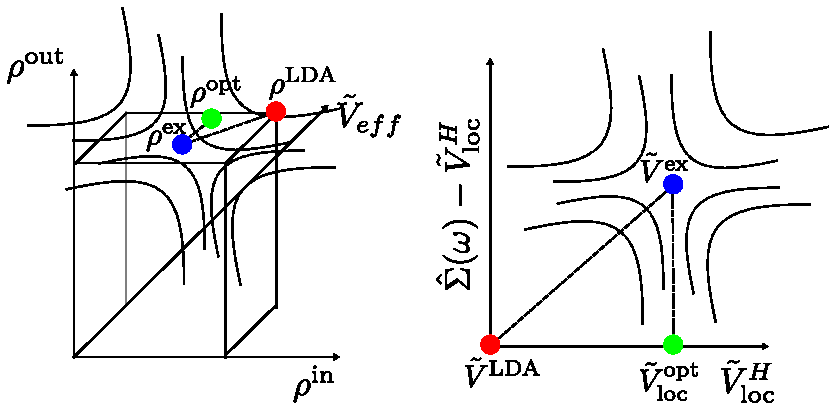
\includegraphics{./GW/HFG_space.pdf}
\caption{Schematic representation of the coordinates for the generalized
Harris-Foulkes functional. Hashed lines represent contours drawn to indicate
a saddle point. The left panel gives stationary points in the co-ordinate space
for different functionals. The blue dot indicates the stationary point for the
LDA Kohn-Sham functional with the exact density $\rho^{ex}$, 
and exact Kohn-Sham energy functional. The green dot gives a stationary point
for a hypothetical "optimal functional". The red dot is a stationary point
for the Kohn-Sham Functional using the local density approximation. The sense in which it is optimal 
is discussed in the text and in Chap.~\ref{chap:manybodyrec}. The
right panel divides the space of effective potentials into a coordinate 
composed of only local Hermitian potentials and an orthogonal co-ordinate 
of non-Hermitian non-local potentials. This is in the spirit of Ref.~\cite{sohrab10}. 
The figure demonstrates how one can approach an optimal
potential which minimizes the distance to the true functional 
while retaining desirable computational properties like being Hermitian and local
or allowing us to avoid multiple iterations to self-consistency.}
\end{center}
\end{figure}
%
The blue dot corresponds to $\rho^{\rm ex}$, and $V^{\rm ex}_{\rm eff}$. The red dot
represents the stationary point for the HKS functional using the LDA.

The important point is that the energy obtained will differ by quantities of second
order smallness in the guessed density, and the effective potential: i.e., 
$(\rho^{\rm in}-\rho^{\rm ex})^{2}$ and $(V_{\rm eff}^{\rm in}-V_{\rm eff}^{\rm ex})^{2}$.
This means with judicious choices we can obtain accurate results with a feasible
amount of computational work.

Finally, the reader may recall the mystery around the first term 
of Eq.~\ref{tb:force} in Chapter~\ref{chap:invariance}. This term is required to complement
the band energy contribution which we can calculate with the recursion technique. However it is
less obvious what form this potential should take. It is often approximated as a pair potential.

If we re-write the total energy following Finnis:
%
%\begin{equation}
%\end{equation}
%
If $\rho_{in}$ in Eq.~\ref{eq:rewrittenHFG} is the charge density for the sum of spherical atomic 
charges then the interacting ion terms will correspond to pair potentials that are rapidly screened. 
These considerations will be developed further in Chapter~\ref{chap:wannier}.

\section{Conclusion}
\noindent
This chapter introduced the Hohenberg-Kohn theorem. This theorem,
which states the ground-state energy of an interacting electronic system 
is a functional of the ground-state charge density is the basis of all the
subsequent discussion. From that theorem much of the rest follows.

The Kohn-Sham scheme was introduced as providing 
a prescription for obtaining a set of wavefunctions, 
and eigenvalues, to describe the ground-state density of a system. 

The various approximations to the exchange correlation 
functional commonly used in applications of Kohn-Sham DFT like the LDA, LDA+U,
GGA, and hybrid functionals are the work horses of materials modelling. 

%For a given configuration of ionsit is commonplace to send a calculation 
%off to a computing machine and within a few
%minutes, hours, or days (depending on the size of the system) come back to directories 
%full of eigenvalues, charge densities, wavefunctions, and total energies.
%We discussed various schemes for extending DFT, a theory for the ground state,
%to describe excited state properties and give us a better treatment of the exchange
%and correlation in real systems. 
We then discussed an approach based on Green's function methods 
to accurately treat processes involving electron addition and removal
to remedy some of the defects present in the use of the local density approximation
to the exchange correlation functional. 

Along these lines we presented a detailed discussion
of the analytic properties of the Green's function and a full derivation of Hedin's
equations which define the $GW$ approximation. Hopefully now the reason it is called
$GW$ is less mysterious \footnote{If the naming remains mysterious you 
should go back and read that section again.}.

The connection to the tight binding formulation of materials science was motivated
in the final section of the $GW$ discussion by sketching out the type of integrals that would 
have to be computed to form the matrix elements of the Green's function and self-energy
operator. The possibility of exploiting a perturbative approach to including
the exchange and correlation energies systematically was discussed in Section~\ref{sec:gwpert}. 
By mapping these operators on to matrix elements and being selective about 
which experimentally accessible quantities we wish to compute 
it should be possible to streamline the calculations into a more manageable framework. 

The formal transformation from DFT/GW methods to functionals
amenable to being described in terms of local short range interactions 
was begun in the section on the Harris-Foulkes functional.
These idea will be developed further in Chapters~\ref{chap:wannier} and \ref{chap:manybodyrec}.

\chapter{Whistlestop Tour of Wannier Functions}
\label{chap:wannier}
\section{A Brief History of Local and Extended Waves}
Chemical intuition is built on a concept of local bonding. 
Yet the mathematics of Bloch waves requires a picture of an 
electron state extended throughout a crystal.
%a figure here of the Pauling dot diagrams of shared bonds
%and a representation of a Bloch orbital would be nice.
Pauling introduced the concept of linear combinations of atomic eigenfunctions
as forming hybrid orbitals which are local and directional in nature and
in many cases can be used to anticipate or explain the observed structure
of molecular compounds \cite{pauling28}. Pauling's publication was contemporaneous
with Felix Bl\"och's work on electrons in crystals \cite{bloch29}. The
way these two perspectives, the local and extended picture of electronic wave functions, 
are applied and rationalized is the distinguishing feature 
in entire fields and sub-fields of physics and chemistry.

The mathematical transformation between the local formulation
and Bl\"och's formulation was obtained by Wannier. 
Wannier succeeded in obtaining a set of functions
from the set of Bl\"och waves which were localized in each unit cell
of a crystal and orthogonal to the wavefunctions in each of its
neighbouring cells \cite{wannier37, wannier62}.\index{Wannier,Bl\"och} 
This work, Wannier noted, was initiated by Eugene Wigner's suggestion that, 
``... there ought to be a way to reconcile the local and the band concept 
for electrons, and that such a reconciliation would probably be useful in 
understanding the spectra of insultators." Koster proposed a variational
procedure for the determination of Wannier functions \cite{koster53},
alongside a number of other early treatments of the problem \cite{winston54}.

The immediate practical consequence of his formalism was
it allowed for an effective computational treatment of impurities 
and donor and acceptor states in semiconductors \cite{slater49,kittel54}.
Appeal to the existence of Wannier like orbitals is frequently made in
tight-binding formulations where they are not explicitly calculated but
matrix elements between them are estimated.

Lennard-Jones evolved a concept of equivalent 
orbitals \cite{lennardjones49a,lennardjones49b, hall50}
to determine the relation between electron-pairing theory of valency, 
the Pauling picture, and the molecular orbital theory treating each 
electron as moving throughout the whole molecular 
framework. Like much of the early work on localized wave functions in molecules 
a group theory formulation of the problem was employed.
In Lennard-Jones' formulation a set of equivalent orbitals, 
if such a set exists, has the property that the effect of a symmetry 
operation only involves the interchange of equivalent orbitals.
See also Kimball for a full statement of the `chemical perspective' 
on orbitals where combinations of spherical harmonics are taken to form
directed bonds \cite{kimball41} with a number of molecular examples.


Lowdin introduced a set of symmetrically orthogonalized wavefunctions which 
can be viewed as an intermediate formulation between hybrid orbitals 
and Wannier functions \cite{lowdin56}.

A unified treatment of each of these perspectives, molecular orbital,
Bloch states, Wannier functions and L\"owdin orbitals based on group theory 
has been made in Ref.~\cite{altmann58}.

\section{MLWF: Maximally Localized Wannier Functions}
For an isolated set N of Bloch bands, in the Maximally Localised Wannier Functions 
(MLWF) formalism, the Wannier function is defined as:
%
\begin{equation}
|w_{n\R}\ket = \frac{V}{(2\pi)^{3}}\int_{\rm BZ} \left[ \sum_{m=1}^{N} U^{\k}_{mn}|\psi_{mk}\ket \right]e^{-i\k\cdot\R}d\k,
\end{equation}
%
where $U_{mn}^{\k}$ rotates the Bloch states at each $\k$-point.

The Maximally Localised Wannier Scheme proceeds by minimizing a spread functional:
%
\begin{equation}
\Omega = \sum_{n}^{N} \left[ \bra r^{2} \ket_{n} - |\bar{\r}|^{2} \right],
\end{equation}
%
a similar criterion for the determination of an optimal basis set for
molecular orbitals was given by Boys and Foster in Ref.~\cite{boys60b}.

Using Blount's relations it can be shown that 
the spread functional can be minimized by rotations of the overlap matrices defined as: 
%\cite{marzari97, mostofi08} 
%
\begin{equation}
M_{mn}^{\k,\bf{b}} = \bra u_{m\k}|u_{n,\k+\bf{b}} \ket.
\end{equation}
%

\subsection{Disentangling Bands}
When we aren't dealing with an isolated set of bands, i.e.
there are broad overlapping bands, e.g. an s-state that crosses in energy
across a group of $d$-like orbitals the procedure of Ref.~\cite{souza02}.
Two windows in energy are defined. An inner energy window of states are frozen 
and a wider set of states in an outer energy window (which contains the smaller
energy window) are projected down into a $N$ vector subspace:
%
\begin{equation}
|u^{\rm opt}_{n\k}\ket = \sum_{m \in N_{\rm win}^{\k}} U_{mn}^{{\rm dis}(\k)}|u_{m\k}\ket
\end{equation}
%

$U^{{\rm dis}(\k)}$ is a rectangular $N_{\rm win}^{\k} \times N$ matrix. 
The subspace is selected by minimising the quantity $\Omega_{I}$ with respect to $U^{{\rm dis}(\k)}$.
Where $\Omega_{I}$ is essentially the variation between neighbouring $\k$-points. 
%
\begin{equation}
\Omega_{I} = \frac{1}{N_{kp}} \sum_{\k, \mathbf{b}} \omega_{b} {\rm tr} \left[\hat{P}_{\k}\hat{Q}_{\k+\mathbf{b}}\right]
\end{equation}

$\hat{P}$ and $\hat{Q}$ are the projection operators: 
$\hat{P}_{\k}=\sum_{n=1}^{N}|u_{n\k}\ket \bra u_{n\k}|$ and $\hat{Q}_{\k} = 1-\hat{P}_{\k}$
minimizing this quantity corresponds to maximizing the overlap between rotated Bloch
states at neighbouring $\k$-points.

Once the optimal subspace has been determined the N vectors are then rotated in the same
was as an isolated set of bands to determine the Wannier function.

\subsection{Hamiltonian in the Wannier Gauge}
In the basis of Bloch wave vectors the Hamiltonian matrix is diagonal at each $\k$ point
with the diagonal element corresponding to the eigenvalue. To rotate to the 
Wannier gauge the optimal rotaion matrix can be used directly:

\begin{equation}
\label{eq:HWan}
H^{W}(\k) = (U^{\k})^{\dagger}(U^{{\rm dis}(\k)})^{\dagger}H(\k)U^{({\rm dis}(\k))}U^{(\k)}.
\end{equation}

$H^{W}$ refers to the Hamiltonian in the Wannier gauge. Eq.~\ref{eq:HWan} can then be contracted
over the $\k$ points to obtain:
%
\begin{equation}
\label{eq:Htb}
H_{nm}(\R) = \frac{1}{N_{\k}} \sum_{\k} e^{-i\k\cdot\R}H_{nm}^{W}(\k).
\end{equation}
%
$H_{nm}(\R)$ corresponds to the matrix elements between Wannier functions at different centers $\R$. 
The matrix elements are generated for the entire grid of supercell vectors $R$ that
are dual to the chosen kpoint. The inverse transform of \ref{eq:Htb} can be used to obtain a
dense $k$-point interpolation of the band structure Ref.~\cite{yates07}.

It is the matrix elements of Eq.~\ref{eq:Htb} that we wish to approximate using a tight binding scheme.
For a tight binding scheme to be valid these elements must decay relatively quickly 
as a function of $\R$ and transform according to the same symmetry operations as spherical harmonics
centered on the atomic sites. 

\subsection{Wanner Practical Procedure}
To carry out the procedure in practice an initial set of orbitals 
${g_{i}(\r)}$ is chosen and the matrix elements:
%
\begin{equation}
\label{eq:overlap}
A^{(\k)}_{mn} = \bra u_{m\k}|g_{n} \ket,
\end{equation}
%
are formed. $A^{\k}_{mn}$ is an $N^{(\k)}_{win} \times N$ matrix. 

A set of N functions at each $\k$ point in the Brillouin zone is given:

\begin{equation}
|\phi_{n\k} \ket = \sum_{m=1}^{N^{(\k)}_{win}} A^{(\k)_{mn}} |u_{m\k}\ket.
\end{equation}

The N functions are then L\"owdin orthogonalized to form an 
initial guess at the projected subspace:
%
\begin{equation}
|u^{\rm opt}_{n\k} \ket = \sum_{m=1}^{N^{\k}_{win}}(AS^{-1/2})_{mn}|u_{m\k}\ket
\end{equation}
%
The initial guess for $U^{\rm dis (\k)}$ is $\mathbf{A}\mathbf{S}^{-1/2}$ 
where $S_{mn}=(A^{\dagger}A)_{mn}$.

Though the minimization is robust a good guess at $g_{i}(\r)$ can speed the process.
For instance for $\alpha$-Fe the appropriate combination of initial states is a combination of 
$d_{xy}$, $d_{zx}$, and $d_{yz}$ orbitals along with 6 $sp^{3}d^{2}$ hybrid orbitals oriented along the 
cubic axes of the crystal. The final MLWFs bear a strong resemblance to these initial states.

The $U^{{\rm dis}(\k)}_{mn}$ matrix evolves from this guess in the course of the 
minimization so that the final rotation matrices at different k-points will have no 
obvious connection with the initial guess. Nor are the Wannier functions diagonal in the basis 
of the trial orbitals. If they were the trial orbitals themselves would be the Wannier functions. 

\section{Symmetry properties of the Wannier Functions}
The appendix of the Slater-Koster paper deals with the issue of whether L\"owdin type
orbitals, which are orthogonalized to their neighbours, transform according to the same
symmetry operations as the spherical harmonics.

\section{TB-NN}
Wannier functions are, it has been pointed out, just a gauge\footnote{What is a gauge?}. But
any gauge that can arrange Bloch orbitals which are spread across a crystal into a localized
packet of orthogonal orbitals will be of some considerable use in the local recursion techniques.
The essential point is that the local Hamiltonians, which the recursion techniques require,
must correspond formally to results obtained {it ab initio}. 
This correspondence must be quantitative and controllable and achieved in 
a way based on rigorous physical reasoning. 
This must be accomplished before we can move on to the real fun with the 
applications in Chapter \ref{eq:}.
Put simply it is essential that the houses are not built on sand! 
It is for this reason Chapter~\ref{chap:gw} contained what it did. The discussion of 
the previous work done on DFT, GW, and the Harris-Foulkes functionals is required to formulate
the local approach.

If they were it would be too easy for another to come along and tweak a few `parameters' to obtain 
new results. 

\section{Diamond Structure TB}
The choice of appropriate basis for a diamond tight binding model requires a little thinking.
The structure itself can be considered a Face Centered Cubic structure with two atoms per unit cell.
The lattice then has atoms at $a(p\bf{i} + q\bf{j} + r\bf{k})$ wherever $p+q+r$ is an even number
as well as at identical points shifted by $\frac{1}{2}a(i+j+k)$. Slater and Koster choose to proceed
by setting up $s,p_{x},p_{y},p_{z}$ orbitals on each of the two sites in a unit cell resulting in 8 
Bloch sums which need to be fit and including interactions between nearest and next nearest neighbours.
The nearest neighbours of one atom consist of a tetrahedral arrangement of atoms belonging to the 
second FCC lattice $a(1/2,1/2,1/2), a(1/2,-1/2,-1/2), a(-1/2,1/2,-1/2), a(-1/2,-1/2,1/2)$,
and 12 second nearest neighbours all located at $a(110)$ positions.

With the Wannier Functions we can choose a different basis. If we choose the origin of our coordinate
system as the center of a nearest neighbour bond between two atoms and set up a face centered cubic lattice
we can choose the eight sp3 wannier functions as a basis and infer the parameters
of their interactions with the 12 nearest neighbour cells of the type a(110). Then instead
of assigning the two center integrals $(ss\sigma)$ etc. to a particular atom, 
i.e. $(ss\sigma)_1$, we assign the two groups to the valence manifold and low lying conduction manifold 
$(ss\sigma)_{v}$. The fitting procedure then seek to fit the disposable constants to the W
annierized Hamiltonian matrix elements. Again a two center approximation can be used in the first pass
resulting in 8 neurons in the hidden layer, and then a second fit which makes use of 
all the disposable constants. The hope is that the MLWF basis will provide an optimal one in the
sense of the rapid spatial decay of the matrix elements between neighbouring unit cells 
(which for sp3 semi-conductors is pracitcally assured), and that the contributions of the three center
integrals will be negligible in this basis. Slater-Koster found that the two center approximation in their
basis was not a particularly good one and unable to interpolate the results obtained
from an orthogonalized plane wave calculation, however the atom centered spherical harmonic orbitals is likely 
to suffer from this deficiency, the requirement that neighbouring orbitals are orthogonal would lead to 
the formation of actual orbitals with non-zero components on neighbouring shells of atoms. 

Choosing the Wannier Basis results in orthogonal orbitals that remain well localized. This approach is similar to
that made by Hall \cite{hall52} who uses symmetric  combinations of directed orbitals
on adjacent pairs of atoms and constructs the bloch sums from these orbitals.
The second nearest neighbour s-interaction is found to have the opposite sign.


%\chapter{Many Body Recursion}
\label{chap:manybodyrecursion}
\section{Introduction}
As mentioned at the close of Chapter.~\ref{chap:invariance} one of the 

The most direct extension of the recursion approach to many body Hamiltonians 
was undertaken In Ref.~\cite{annett94}. The concept of the local density of states (LDOS)
is extended to the projected density of transitions (PDOT) and it is argued singularities
in the PDoT correspond to thresholds for creating long lived elementary excitations 
in the many body system. In this chapter we demonstrate how to map a GW type calculation
on to a chain model. The analogy between an impurity or adsorbed atom interacting with
a constant chain and single particle states interacting via plasmon excitations is 
also pointed out the plasmon band serving to renormalize the single particle state.
The important calculations are then the position and bandwidth of the interaction
bands and the coupling of the single particle states to the interaction bands.
Efficient schemes for computing the positions of the interactions bands and 
their coupling to the single particle states (represented as Wannier functions)
are discussed.

Mapping the interacting problem to chain models means larger configurations can be studied
and the positions of band edges and defect states can be computed.

\section{Recursive GW}
We write down the many body Hamiltonian amenable in a manageable form:
%
\begin{equation}
\hat{H} = [-\frac{1}{2}\nabla^{2} + \tilde{v}_{\rm loc} + \hat{\Sigma}(\r,\r';\omega)]
\end{equation}
%
	$\Sigma(\r,\r';\omega)$ is a self energy operator, it is not local and 
has an additional argument that includes the energy.

The on-site self-interaction term can be computed as:
%
\begin{equation}
a_{0}(\omega) = \int\int\bra w_{i}(\r-\R_{i})|\hat{\Sigma}(\r,\r';\omega)|w_{i}(\r'-\R_{i})\ket d\r'd\r.
\end{equation}
%

The off diagonal elements of a tight binding Hamiltonian can be written as:
%
\begin{equation}
b_{ij}(w) = \int\int\bra w_{i}(\r-\R)|\hat{\Sigma}(\r,\r';\omega)|w_{j}(\r'-\R_{j})\ket d\r d\r'
\end{equation}
%
	Subsequent neighbour interactions would take a similar form
with the integration region, $\Omega_{j}$ being a Wigner cell around an 
atom with its Wannier center at $\R_j$. In order for the scheme to be sensible 
the contributions from subsequent shells must be negligible. This is likely 
to be the case so long as either the atomic orbitals $w$ and/or $\Sigma$ 
fall off quickly enough. Which, as will become clear when we discuss
the relationship of this scheme to the GW approximation, requires 
the Green's function or the screened Coulomb interaction to be sufficiently localized.

%
The self-consistency in the recursion method relies on the adjustment of the coefficients that
define the Green's function. If a suitable non interacting Hamiltonian is selected in the first
place this self-consistency can be treated as a perturbation problem.

In principle we can now compute any quantity we like that can be expressed
as a density of states, or an integral over the DOS, with the Many-Body Green's 
function just as in the non-interacting case discussed in Chap.~\ref{chap:invariance}.

%
%The link then has to come to Mori for random forces/coherent forces
%resulting in the emergence of the dielectric constant, plasmon frequency etc.
%
%The test case for this would be with Si, if 
%I can reproduce spectral functions with TB recursion that is a legitimate 
%proof of concept and would clarify the extent to which collective excitations,
%plasmons etc., can be incorporated in TB recursion. 
%


\section{The Self-Energy From Multiple Greenian Elements}
  A good first order approximation to $\Sigma$ comes from the GW approximation.
We will write matrix elements of this to see the connection between the
recursion method and the calculation of $\Sigma$. It should be come apparent that computing
the self-energy requires a large table of Greenian matrix elements between states localized
on nearby atoms, far away atoms, and the entire valence and conduction band spectrums. 
This table of Greenian elements could become excessively large very quickly and requires some
rigorous procedure to map it back into a manageable scale.
%
\begin{equation}
\label{eq:sigma}
\Sigma_{ij}(\omega) = \bra\phi_{i}|\int G(\omega-\omega')W(\omega')d\omega'|\phi_{j}\ket
\end{equation}
%
We now insert the identity operator into Eq.$\sigma$ strategically and at a number of places:
%
\begin{equation}
\label{eq:sigma}
\Sigma_{ij}(\omega) = \bra\phi_{i}|\int G(\omega')\sum_{n}|\phi_{n}\ket\bra\phi_{n}|(G(\omega')|\phi_{n}\ket\bra\phi_{n}|G(-\omega')v)d\omega'|\phi_{j}\ket
\end{equation}
%
\begin{equation}
\label{eq:sigma_onsite}%need to check the frequency polarization expression
\Sigma_{ii}(\omega) = \bra\phi_{i}|\int G(\omega')\sum_{n}|\phi_{n}\ket\bra\phi_{n}|(G(\omega')|\phi_{n}\ket\bra\phi_{n}|G(-\omega')v)d\omega'|\phi_{i}\ket
\end{equation}
%
The insertion of multiple identity operators makes what we need clear. What is required 
is to tabulate the Greenian's, $G_{ij}(\omega)$, between eigenstates of the system
the non-interacting system. In {\it ab initio} calculations this requirement 
gives rise to the "sum over states" problem. Although in principle the valence
and conduction states, at every wave vector, are known their calculation and storage
is tedious, and justified truncation of the sum is problematic.

For this scheme to be workable we again stress that the system interaction
must be sufficiently local such that $\Sigma_{ij}$ matrix elements can be
calculated. This corresponds to the mutual interaction of the electrons being 
short ranged. For a single particle tight binding model these off diagonal hopping
elements can be calculated and are fixed. It is this interaction we wish
to generalize slightly to allow for a component of dynamical interaction.
\section{The Project Density of Transitions}
The PDOT\cite{annett93, haydock00, haydock16} method is 
appropriate for calculating the polarizability and provides a direct physical
interpretation in a many electron system. 

Written in Hedin's scheme the polarizability 
takes the form of a term: $iGG$, in Feynman diagrams this is a bubble diagram. We need to calculate the propagator
of an electron from 1 to 2, and a hole from 2 to 1. Dimensionally, after a Fourier transform,
the polarizability has units of transition probability per unit energy. Where there are discrete
states there are discrete transitions, this would be the case for systems
that could be considered molecules, where there are continuous bands there are continuous
bands of transitions, in metallic crystals this would be the case.

Where the recursion method for the PDOS computes the final energy distribution
for a stationary state in the syste


I think Umari's operator for $|\phi\ket\bra\phi|$ would be a natural way of
approximating the necessary sums that are complimentary to the chosen
localized single particle states (both valence and low lying conduction).
We then have the continuum states as $|\phi\ket=e^{i\G\cdot\r}-<\G|w_{i}(\r-\R)>$,
with the occupied and low lying conduction manifold represented as Wannier 
functions and the $|\phi>$ states as orthogonalized plane waves.

	Although this is essentially just a rewriting of Hedin's equations
it has practical consequences. The present method eliminates
burdensome storage of what are in practice gigantic Green's function, 
screened Coulomb, and self-energy matrices. It also 
stabilizes the necessary numerical integrations and convolutions in frequency space. 
The quadrature methods used in the standard recursion theory remain applicable.

These savings are obtained at the price of a nested call stack of recursions which 
in principle must be infinite. This may seem troubling but we do intend to truncate
the level of recursion at some point and the depth of the recursive call stack should
equate to the number of terms in the self energy expansion that are required.

	Careful, justified, selection of the initial wave functions and tight binding parameters
is also required and these quantities (if they are not chosen to be analytic and approximate)
must be computed and stored. However work done on Wannier functions makes this a very
practical route. We will now embark on some numerical work in the hope that satisfactory 
results can be obtained by truncation of the recursive call stack at a manageable level. 

Finally the method requires computation of the initial stationary states of the system.

The electron addition operator:
%
\begin{equation}
[H, c^{\dagger}(t)] = -i\hbar \frac{d}{dt} c^{\dagger}(t).
\end{equation}
%
The operator will evolve into a superposition of a fraction of the 
possible transitions of the system. If a complete set of orthonormal $\{P_{\zeta}\}$ 
states is introduced the projected transitions can be written:
%
\begin{equation}
\psi_{\alpha} = \sum_{\zeta\eta} P_{\zeta}c^{\dagger}P_{\eta} \qquad \epsilon_{\alpha} = E_{\zeta} - E_{\eta}
\end{equation}
%
The PDOT is then:
%
\begin{equation}
\label{eq:ehpairs}
\mu(\epsilon) = \sum_{\alpha} \bra\psi_{\alpha}^{\dagger}|\psi_{\alpha}\ket \delta(\epsilon-\epsilon_{\alpha})
\end{equation}
%
The stationary states all have infinite lifetimes, and according to Haydock, \ref{eq:ehpairs} can
be interpreted as the probability distribution in energy for the decay of a bare electron into one dressed
with electron-hole pairs.

It is possible to formulate this in terms of discrete transitions for low energies, for high energies
the initial state is clearly going to diffuse outwards very far and result in the excitation of 
many oscillators throughout the crystal. Where the complete set of orthonormal states
hasn't been computed already (this refers to the sum over states problem) it is required to directly
calculate the PDOT. Haydock gives a prescription for this the time dependent behaviour of
an operator is given:
%
\begin{equation}
\label{eq:creationt}
c^{\dagger}(t) = e^{i\mathbf{L}t/\hbar} c^{\dagger}
\end{equation}
%

$\mathbf{L}$, the Liouvillian, is defined as a superoperator which
acts on an operator $\mathbf{x}$ as:
%
\begin{equation}
\mathbf{L} \mathbf{x} = [\mathbf{H}, \mathbf{x}]
\end{equation}
%
Eq.~\ref{eq:creationt} generates an expanding set of operators similar to what we encountered
in Chap.~\ref{chap:gw} at Eq.~\ref{eq:2pgreenfxn} where the field operators kept coupling
together as we expanded the many body interaction. Being able to truncate this expansion
rigorously is something we would like to do.

We would like to compare the mechanics discussed in the the project density of transitions
to Hedin's GW approximation, and provides a framework for computing the renormalization 
in terms of local orbitals and effective energy bands.

With the choices $u_{0}=c^{\dagger}/<c c^{\dagger}>^{\frac{1}{2}}$, and $u_{-1}=0$,
subsequent operators are:
%
\begin{equation}
\label{eq:pdotvectors}
\mathbf{u}_{n+1} = (\mathbf{L} \mathbf{u}_{n} - a_{n}-b_{n}\mathbf{u}_{n-1})/b_{n+1}
\end{equation}
%
\begin{equation}
a_{n} = \bra u^{\dagger}_{n} \mathbf{L} \mathbf{u}_{n} \ket
\end{equation}
%
\begin{equation}
b_{n+1} = \bra 
(\mathbf{L} \mathbf{u}_{n} - a_{n} \mathbf{u}_{n} - b_{n}u_{n-1})^{\dagger} 
(\mathbf{L} \mathbf{u}_{n} - a_{n} \mathbf{u}_{n} - b_{n}u_{n-1})
\ket^{\frac{1}{2}}
\end{equation}
%

Like conjugate gradients this recursion rarely terminates in practice 
due to loss of orthogonality of the vectors or because the subspace is 
too large to compute.

Where the charge density oscillations are on an interatomic scale of distance
we talk about single particle excitations, where they are across multiple 
interatomic spacings we speak of charge density oscillations and plasmons.

If the PDoT consists of a single band of transitions with a known width 
and energy,then the recurrence can be continued with constant matrix elements, $a_{n}$ and $b_{n}=b$
for $n>N$ where a and b are fit to the known band. 

For interacting bands it becomes more difficult to approximate a 
single effective energy band.

The termination of the recurrence is a very important point. 
We are interested in the excited state properties of an N+1 or N-1 electron system
from a local perspective. In Chapter.~\ref{chap:invariance} we worked hard to collect work
justifying this perspective. 

In a continued fraction expansion of the the PDoT more and more distance transitions are coupled
to the starting transition. In a real system the continued fraction will terminate at the surface,
however if the surface atom is changed by a small number of atomic positions it would
be somewhat surprising, and very interesting, if this had a strong effect on the electronic
properties around an atom deep in the cavity. Picking a value of anywhere from 30-60 moments 
away from a starting atom should help the reader to visualize this.

For silicon, the plasmon energy band occurs around 16 eV. This is very high compared
to the single particle excitations which occur around 1 eV. The long range $1/r$ nature of the Coulomb
interaction means electrons are coupled over large distances.
This coupling accounts for the high excitation energy: to get the
electron cloud moving collectively requires a relatively large amount of energy.

Experience with the GW approximation indicates an effective band model works very well
for sp semiconductors \cite{godbyneeds, hybertsenlouie, bergstressen}. 
A single plasmon mode approximates the long range density of transitions, and the local
atomic environment contributions to the PDoT can then be captured directly with the standard nearest
neighbour hopping and the inclusion of the lowest energy single particle transitions.

The situation for transition metals will be more complicated but again the local approach should yield 
a tractable framework. The important low energy transitions can all be included 
as explicit single particle states in the Hamiltonian (spin resolved states). 
The remaining particle-hole renormalization would then be accounted for 
via a set of effective plasmon energy bands. It would be of interest to
see how the number and position of these effective bands can change between systems.

The projected transitions can be written:
%
\begin{equation}
\mathbf{\psi}_{\alpha} = \sum_{n} \psi_{n}(\epsilon_{\alpha})\mathbf{u}_{n}
\end{equation}
%
the sum is over the basis ${\mathbf{u}_{n}}$ generated by Eq.~\ref{eq:pdotvectors}
with coefficients generated by:

\begin{equation}
\label{eq:pdotcoeff}
\psi_{n+1}(\epsilon) = ((\epsilon-a_{n})\psi_{n}(\epsilon) - b_{n}\psi_{n-1}(\epsilon))/b_{n+1}
\end{equation}

In his paper Haydock says equation \ref{eq:pdotcoeff} has two linearly independent solutions
which can be combined to satisfy the boundary conditions on $\psi_{N+1}$ or $\psi_{-1}$ or both.
Physically I understand this as choosing where the recurrence begins and ends not completely
clear on what it implies mathematically.

The $\mathbf{u}_{0}-\mathbf{u}_{0}$ element of the resolvent is:
%
\begin{eqnarray}
R(\epsilon)& = & 1/\epsilon-a_{0}-b_{1}\psi_{1}(\epsilon)/\psi_{0}(\epsilon) \\
  & = & 1/\epsilon-a_{0}-b^{2}_{1}\epsilon-a_{1}-b^{2}_{2}\epsilon...b_{n}^{2}/\epsilon-a_{n},
\end{eqnarray}
%
and finally the PDoT:
%
\begin{equation}
\mu(\epsilon) = -\bra \mathbf{c} \mathbf{c}^{\dagger}\ket {\rm Sing} \frac{R(\epsilon)}{2\pi i}
\end{equation}
%
The PDoT is the residue of the resolvent which contributes to integrals enclosing the 
real $\epsilon$-line and it is normalized to the projecting operator.

Calculating how much of the sum rule is exhausted will give a good indication
of the effectiveness of a single band approximation, or what is equivalent,
the truncation of the recursion at a suitable number of moments.

Finally a note from the perspective of plane waves and pseudopotentials. For
highly excited conduction band states. The Bloch periodic wave function is
essentially a plane wave or free electron state. This is equivalent to saying for
sufficiently high energy states the kinetic energy is the dominant term in the Hamiltonian.
For these plane wave states the Wannier transformation is a psinc function. These psincs
give a local representation of high energy plasmon modes.

\section{Appeal of A Local Formulation of Many Body Quantum Systems}
 A resonance or transition in k-space corresponds to an excitation 
of a crystalline eigenstate but the physical meaning of this is hard to access. Highly
localized states in $\k$-space correspond to relatively diffuse regions in real space. Where
transitions are formulated in terms of the local atomic environment the process becomes slightly
more intuitive. An electron creation/destruction operator $u_{0}$ places/removes an electron in the 
first available excited/occupied state with eigenvalue $a_{0}$ in a particular unit cell. 
In terms of energy the operator takes the system to the energy 
of the $E_{N\pm1}$ interacting system. 

Eq.~\ref{eq:pdotvectors} will contain the contributions of the localized
wave packets in a vector $u_{\alpha}$ that corresponds to the resonance 
$\epsilon_{\alpha}$. In an inverse photoemission experiment the $u_{\alpha}$ chain
will come from the commutator of an electron creation operator, for a photoemission
experiment the chain of vectors in the excitation will correspond to creating a hole
in the electron system. An electronic wave packet interacts with its neighbours becoming
``dressed" by the nearby excitations of electron hole pairs. 

In a photoemission experiment real electric currents will be moving through the crystal as well.
Only the $\k$-component of the localized wave packet, at a given energy, will move through the crystal as 
an approximate eigenstate and can pass through without scattering so much that it can't be detected.
When the wave packet reaches the surface it can continue propagating
or be scattered back into the crystal, if it is to continue propagating the appropriate matrix element
is between the plane wave of the appropriate wave vector and the localized wave packet along with some
surface potential.

Other processes mean the excited state can hop 
to its nearest neighbour leaving behind a hole. The recursive formula means
the coefficients of the continued fraction and the vectors are generated at
each step and the energy dependence of the interaction can be calculated 
in a closed form. The trade off is the recursion depth must be sufficient to
pick up all the relevant poles of the interaction. For collective modes
the recursion depth would have to proceed to an impracticable depth which
is why we must map these contributions onto effective energy bands, collective
variables, or plasmon modes (depending on how you prefer to call them). 
The technique demonstrates the mathematical and physical justification 
of the plasmon as a mathematical transformation or collective excitation.

The hole state and the excited state will also interact according 
to the Coulomb interaction, these are excitons, the radius of their (potentially) 
bound state being determined by the strength of the screened coulomb interaction 
and the shapes of the electron and hole wave function. 
However the PDoT we are considering at the moment is just a single electron creation operator.
To calculate the PDoT for the electron hole system would require a 
two particle Green's function operator with a new pole in the spectrum forming
at the energy of the electron hole bound state.

\section{Mori Memory Function}
\label{sec:morimemory}
  As noted in Ref.~\cite{annett94} there is a close connection between the PDOT
formalism and Mori's memory function. 

%Interestingly when working on the diffusion
%of hydrogen in a lattice I realised I would require a way of computing the
%inverse Laplace transform of the continued fraction generated 
%using Haydock's method. A quick search later and one of the first items to come up
%was a paper titled "A Continued-Fraction Representation of the Time-Correlation
%Functions" the first line of the abstract was, "A continued-fraction expansion of the Laplace
%transform of the time-correlation functions is obtained...". It is very nice when a problem
%arises where all you have to do is go to the shop and grab the solution off the shelf.

%Like many store bought items some element of self-assembly is required. In this
%section we wish to simplify Mori's analysis as much as possible so that we can directly 
%apply the mathematical machinery of translating a continued fraction representation of
%a diffusion problem into the time domain and extract measurable quantities.

The inner product, or matrix elements required to generate the coefficients 
$a_{n}$ and $b_{n}$ in Mori's approach are generalized to include a thermal averaging:
%\begin{equation}
%\label{eq:moriinner}
%(F, G^{*})= \frac{1}{\beta} \int_{0}^{\beta} \bra e^{\lambda H)F e^{-\lambda H}G^{*}\ket d\lambda
%\end{equation}
There is a further computational advantage here. Though the inner product in Eq.\ref{eq:moriinner}
looks complicated, in fact, it only has the effect of altering the coefficients entering
the hopping matrix. This means the laplace transform computed from the continued fraction,
and the quantum mechanical hopping parameters can be computed separately.

Mori's formula allows us to interpret the spectral function in two ways. The first is as
a purely phenomenological one of an electron in a material being excited and as it passes through
a crystal on the way to a detector being scattered by the characteristic scattering modes of the
system. The electron from its initial bound state can interact with the many body system via
the plasmon modes available to it.

The second is to interpret the probe as measuring a statistical distribution of the 
renormalized many-body electron states which have spectral weight across the full
interacting energy spectrum. 

The former is similar to the treatment of a molecules path
being modified by its collisions with atoms in what is termed Brownian motion. In the
case of a fermion in a crystal we are looking at its `Brownian motion' as it interacts
with bosons on its way to a detector. 

\section{Phase Transitions}
The parameters $\omega_{j}$ and $\Delta^{2}_{j}$ are writen in terms static
correlation functions some of them may have an anomalous temperature dependence.

\section{Applications }
GW type calculations are important for electron addition and removal 
experiments. We investigate the GW-recursion type calculations for 
impurities in Si. For data on this see Refs.~\cite{lehto78}.

%Perturbations:
%Haydock J. Phys. A Vol. 10, No. 4 (1977)
%Susceptibilities
%K. Terakura, J. Phys. C 11 469 (1978)

\chapter{Superconductivity}
\label{chap:superconductivity}
Superconductivity is probably the most incredible physical phenomenon. 

\section{Experimental Data}
The experimental data gives some sense of the superconducting
phenomenon \cite{teuser59}.

\section{Calculating $\mu$, $\mu^{*}$}
Since Bogoliubov the screened Coulomb interaction is 
included in calculations on superconductivity assuming 
it acts like a hard core and is ineffective in 
weakening the phonon-induced attraction.

In Ref.~\cite{morel62} the exact Coulomb interaction is modeled 
as an instantaneous potential, neglecting high-order retarded polarization terms. 
They justify this by saying that dispersion occurs only at rather
high frequencies of the order of the plasma frequency 
and is completely negligible in the small energy range around the Fermi surface.

The instantaneous acting Coulomb interaction is considered 
equivalent to adding a constant to the frequency dependent potential.
%
\begin{equation}
U^{'}(\omega) = \lambda U(\omega) - \mu
\end{equation}
%
Where $\mu$ is the angular average of the Coulomb potential $V(\q)$:
%
\begin{equation}
\mu=\frac{1}{4\pi^{2}v_{0}}\int_{0}^{2k_{0}}\frac{4\pi e^{2}}{k_{s}^{2}+q^{2}}qdq
\end{equation}
%
\begin{equation}
\mu=\frac{k_{s}^{2}}{8k_{0}^{2}}\ln\left[\frac{4k_{0}^{2}+k_{s}^{2}}{k_{s}^{2}}\right]
\end{equation}

$v_{0}$ is the Fermi velocity, $k_{0}$ is the fermi momentum, $k_{s}$ is the screening
wave vector (in a Thomas-Fermi model this would be proportional to the density of states).

If we use the Thomas-Fermi model then: 
%
\begin{equation}
a^{2} = \frac{k^{2}_{s}}{4k^{2}_{0}} = 4\pi e^{2} N_{0}/4k^{2}_{0}
\end{equation}
%
\begin{equation}
\mu = \frac{1}{2} \ln \left[(1+a^{2})/a^{2}\right]
\end{equation}

Just as a note on phonons:
%
\begin{equation}
\lambda = \int_{0}^{1}\left[ \frac{a^{2}}{a^{2} + q^{2}/4k^{2}_{0}}\right]^{2} x dx
\end{equation}
%
where $x=|\k-\k'|/2k_{0}$.

Local fields can be ignored for alkali metals so:
%
\begin{equation}
\lambda \approx \int_{0}^{1} \left[\frac{a^{2}}{a^{2}+x^{2}}\right]^{2}x dx=\frac{1}{2}\frac{a^{2}}{1+a^{2}}
\end{equation}
%
\begin{figure}
\label{fig:supercond}
\begin{center}
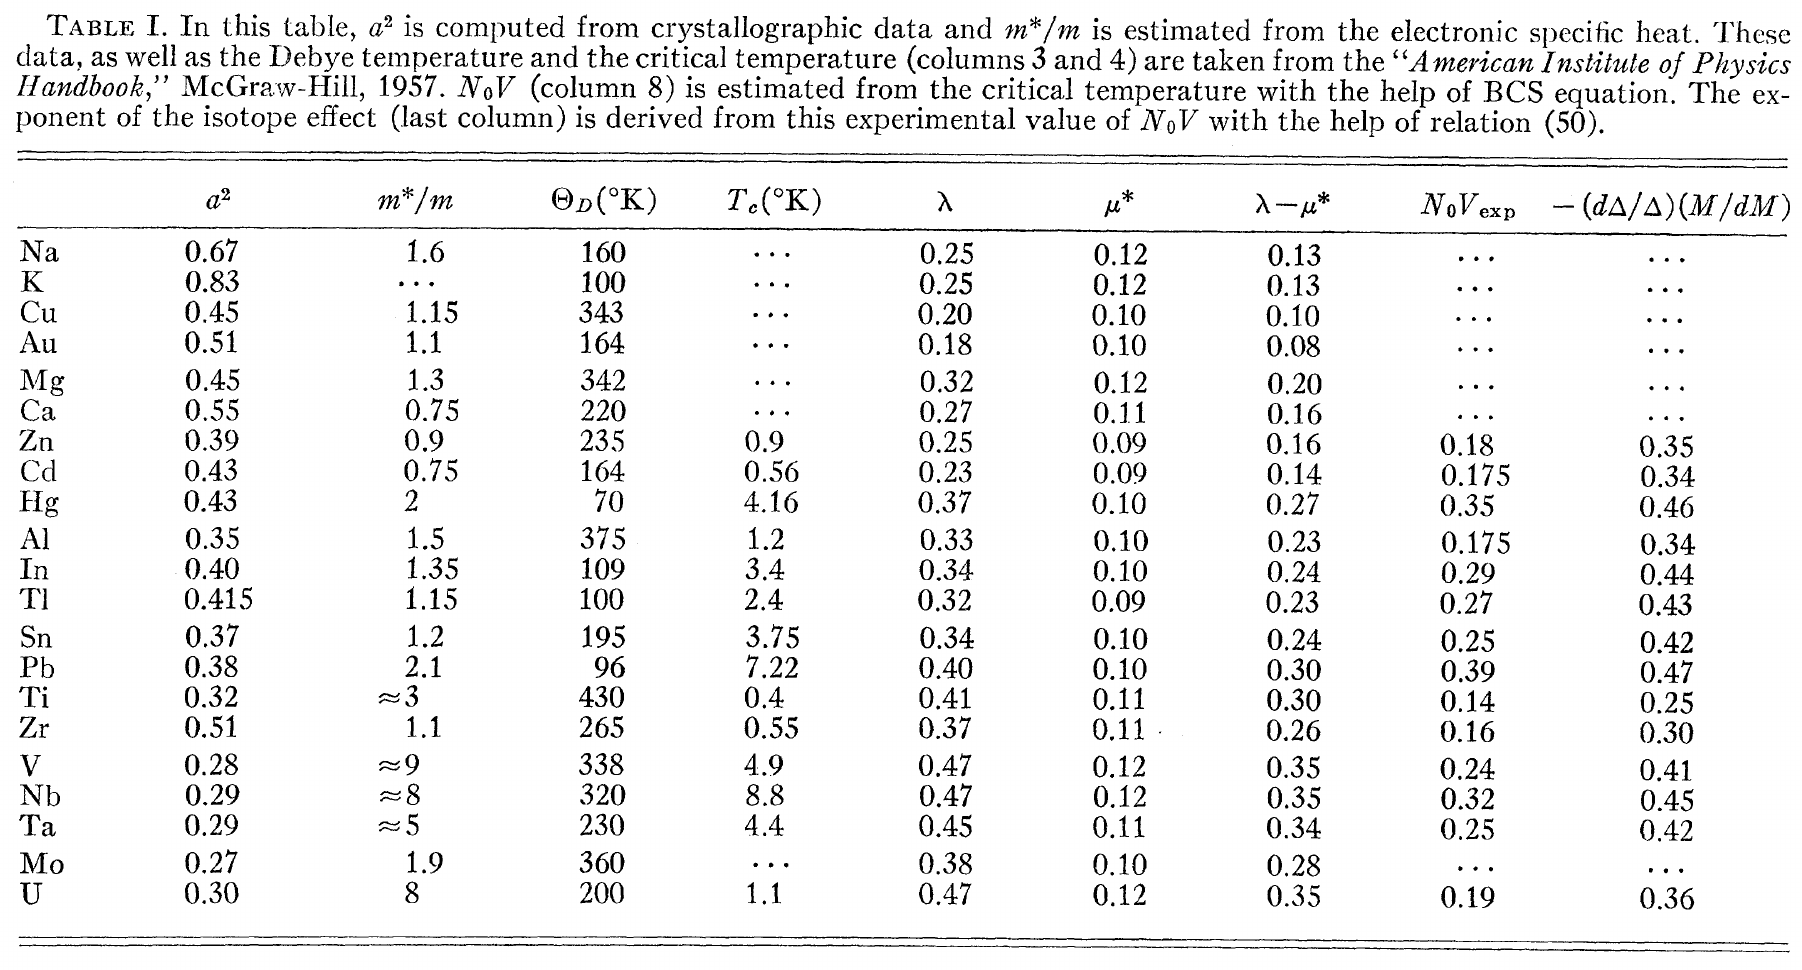
\includegraphics[height=50mm]{./Superconductivity/superconductingparameters.png}
\caption{\small Superconductivity}
\end{center}
\end{figure}
%
When the Coulomb screening is included in the equations for the 
superconducting gap it is modified to be:
%
\begin{equation}
\mu^{*} =  \frac{\mu}{1+ \mu \ln(\frac{\epsilon_{F}}{\theta_{D}})}
\end{equation}
%
\section{Dielectric Matrix Elements}
The above was derived using analytic models in the 60s. Since we have access
to the Fermi surfaces, etc. we can build a more sophisticated model of the
microscopic screening.

The Coulomb repulsion parameter $\mu$ is the Fermi surface average of the Coulomb
scattering matrix elements, $V^{c}_{\k\k'}$:
%
\begin{equation}
\label{eq:fsavg}
\mu = N(0) \bra\bra V^{c}_{\k\k'} \ket\ket_{FS}.
\end{equation}
%

Eq.~\ref{eq:fsavg} can be written explicitly as:
%
\begin{equation}
\mu = \frac{1}{N(0)} \sum_{n\k}\sum_{n'\k'}V^{c}_{n\k,n'\k'}\delta(\epsilon_{n\k}-\epsilon_{F})\delta(\epsilon_{n'\k'}-\epsilon_{F}).
\end{equation}
%

%
\begin{equation}
V^{c}_{n\k,n'\k'} = \bra n'\k'\uparrow, n'-\k'\downarrow |V^{c}| n\k\uparrow, 
n-\k\downarrow\ket
\end{equation}
%
\begin{equation}
V^{c}_{n\k,n'\k'} = \int \psi^{*}_{n'\k'}(\r)\psi^{*}_{n'-\k'}(\r') V^{c}(\r,\r')
\psi_{n\k}(\r)\psi_{n-\k}(\r')\:\rm{d}\r\mathrm{d}\r'
\end{equation}
%

\subsection{Coulomb matrix elements in $\G$ space}
In Ref.~\cite{cohen95} the reciprocal space matrix elements are given.
%
\begin{equation}
\label{eq:cohen1}
V^{c}_{n\k,n'\k'} = \sum_{\G\G'}f^{*}_{n\k,n'\k'}(\G)\epsilon^{-1}(\q+\G,\q+\G')
\times \frac{4\pi e^{2}}{\Omega|\q+\G'|^{2}}f_{n\k,n'\k'}(\G'),
\end{equation}

where $\Omega$ is the crystal volume and $f_{n\k,n'\k'}$ is:
%
\begin{equation}
\label{eq:cohen2}
f_{n\k,n'\k'}(\G) = \sum_{\G'} \psi_{n'\k'}(\G+\G')\psi^{*}_{n\k}(\G')
\end{equation}
%

\subsection{Coulomb matrix elements in SGW}
The convention for two point functions is:
%
\begin{equation}\label{eq.fourier}
 F(\r,\r',\w) = \frac{1}{N_\k\Omega}  \sum_{\k,\G\G'} 
  {\rm e}^{-i(\k+\G)\cdot\r} 
  f_{[\k,\G,\w]}(\G')
  {\rm e}^{i(\k+\G')\cdot\r'}.
\end{equation}
%
The wave function convention for bloch wavefunctions is:
%
\begin{equation}
\psi_{n\k}(\r) = \frac{1}{\sqrt{\Omega}}\sum_{\G}u_{n\k}(\G)e^{i(\k+\G)\cdot\r},
\end{equation}

We have a different sign convention on W so it might be better to rederive
Eqs.~\ref{eq:cohen1} and \ref{eq:cohen2} independently.
%
\begin{equation}
V^{c}_{n\k,n'\k'} = \int \int \psi^{*}_{n'\k'}(\r)\psi_{n\k}(\r)V^{c}(\r,\r')\psi^{*}_{n'-\k'}(\r')\psi_{n-\k}(\r')\rm{d}\r \rm{d}\r'
\end{equation}
%
\begin{equation}
V^{c}(\r,\r') = \frac{1}{N_{\q}\Omega}\sum_{\q,\G,\G'}e^{-i(\q+\G)\cdot\r} \epsilon^{-1}_{\G\G'}(\q,\omega=0)\frac{4\pi e^{2}}{|\q+\G|^{2}} e^{i(\q+\G')\cdot\r'}
\end{equation}
%
First we will do the integral over $\rm{d}\r$ to obtain the constraints on $\q,\G,\G_{1},\G_{2}$:
%
\begin{equation}
V^{c}_{n\k,n'\k'} = \int \int \sum_{\q,\G,\G_{1},\G_{2}} e^{-i(\k'+\q-\k)\cdot\r} e^{-i(\G+\G_{2}-\G_{1})\cdot\r} u^{*}_{n'\k'}(\G) u_{n\k}(\G_{1})\\
\frac{4\pi e^{2}\epsilon^{-1}_{\G_{2}\G_{2}'}}{|\q+\G_{2}|^{2}}...\rm{d}\r\rm{d}\r'.
\end{equation}
%
Then integrating over $\rm{d}\r'$:
%
\begin{multline}
V^{c}_{n\k,n'\k'} = \sum_{\q,\G,\G_{1},\G_{2}} \delta(\k'+\q-\k) \delta(\G+\G_{2}-\G_{1}) u^{*}_{n'\k'}(\G)u_{n\k}(\G_{1})\\
\int \sum_{\G',\G_{1}'\G_{2}'} \frac{4\pi e^{2}\epsilon^{-1}_{\G_{2}\G_{2}'}(\q,\omega=0)}{|\q+\G_{2}|^{2}}
e^{-i(\k-\k'-\q)\cdot\r'} e^{i(\G_{1}'+\G_{2}'-\G')}u^{*}_{n'-\k'}(\G') u_{n-\k}(\G_{1}')\rm{d}\r',
\end{multline}
%
we find:
%
\begin{multline}
V^{c}_{n\k,n'\k'} = \sum_{\q,\G,\G_{1},\G_{2}}\sum_{\G',\G_{1}'\G_{2}'} \delta(\k'+\q-\k)\delta(\G+\G_{2}-\G_{1})\delta(\k-\k'-\q)\delta(\G_{1}'+\G_{2}'-\G')\\ 
u^{*}_{n'\k'}(\G)u_{n\k}(\G_{1})\frac{4\pi e^{2}\epsilon^{-1}_{\G_{2}\G_{2}'}(\q,\omega=0)}{|\q+\G|^{2}} u^{*}_{n'-\k'}(\G')u_{n-\k}(\G_{1}')
\end{multline}

The first constraint on the wave vectors in the brillouin zone is $\q=\k-\k'$. So the change in sign convention
on the dielectric function from Ref.~\cite{cohen95} just means we switch $\k$ and $\k'$. The second
constraint is $\G_{1} = \G + \G_{2}$, and the third constraint is $\G^{'}=\G_{2}+\G_{1}'$. Making
these substitutions we find (multiplying by a $1/\Omega$): 
%
\begin{equation}
V^{c}_{n\k,n'\k'} = \frac{1}{N_{\q}\Omega}\sum_{\G,\G_{2}}\sum_{\G_{1}',\G_{2}'} u^{*}_{n'\k'}(\G)u_{n\k}(\G+\G_{2})
\frac{4\pi e^{2}\epsilon^{-1}_{\G_{2}\G_{2}'}(\q,\omega=0)}{|\q+\G_{2}|^{2}}u^{*}_{n'-\k'}(\G_{1}'+\G_{2}')u_{n-\k}(\G_{1}')
\end{equation}
%
Finally we can introduce the function:
%
\begin{equation}
f_{n'\k',n\k}(\G_{2})= \sum_{\G} u^{*}_{n'\k'}(\G)u_{n\k}(\G+\G_{2})
\end{equation}
%
Or relabeling $\G_{2}=\G$ and $\G=\G'$ we find:
%
\begin{equation}
f_{n'\k',n\k}(\G)= \sum_{\G'} u^{*}_{n'\k'}(\G')u_{n\k}(\G+\G')
\end{equation}
%
If we use time reversal symmetry then we 
recover the expression in Eq.~\ref{eq:cohen2}.
Instead of convolving in $\G$~space it is more convenient to do the products of the
wave functions in real space then apply the dielectric function in $\G$~space:
%
\begin{equation}
f_{n'\k',n\k}(\G) = \int e^{-i(\G\cdot\r)} \psi_{n'\k'}(\r)\psi_{n\k}(\r) \rm{d}\r
\end{equation}
%
Let us resolve $\k'=\k-\q$:
%
\begin{equation}
V^{c}_{n\k,n'\k-\q} = \frac{1}{N_{\q}\Omega}\sum_{\G,\G'}f^{*}_{n'\k-\q,n\k}(\G)
\frac{4\pi e^{2}\epsilon^{-1}_{\G\G'}(\q,\omega=0)}{|\q+\G|^{2}}f_{n'-(\k-\q),n-\k}(\G')
\end{equation}
%
\section{Fermi Surface Average}
Once we are in possession of the matrix elements they must be averaged over the Fermi surface:
%
\begin{equation}
\mu = \frac{1}{N(0)} \sum_{n\k}\sum_{n'\k'}V^{c}_{n\k,n'\k'}\delta(\epsilon_{n\k}-\epsilon_{F})\delta(\epsilon_{n'\k'}-\epsilon_{F}).
\end{equation}
%
$N(0)$ is the density of states per spin at the Fermi energy $\epsilon_{F}$.

The average can be performed using the linear tetrahedron method of Ref.~\cite{lehmann72} or the
the more recent method proposed by Bl\"ochl Ref.~\cite{blochl94}.

\section{Dielectric functions}
\subsection{Lindhard Dielectric Function}
Mahan (may his tribe increase) gives the RPA dielectric function in the static limit:
%
\begin{equation}
\label{eq:statlindhard}
\epsilon(\q,0) = 1 + \frac{q^{2}_{TF}}{2q^{2}}\left[1+\frac{1}{2x}(1-x^{2})\ln\left|\frac{1+x}{1-x}\right|\right]
\end{equation}
%
where $x = q/2k_{F}$.
Eq.~\ref{eq:statlindhard} is what we will use to test our Fermi averaged Coulomb matrix elements.

\subsection{Hubbard Dielectric Function}
The Hubbard dielectric function introduces a correction factor to the RPA of the form:
%
\begin{equation}
\epsilon_{H}(\q,\omega) = 1 - \frac{v_{q}P^{1}(\q,\omega)}{1+ v_{q}G_{H}(\q)P^{1}(\q,\omega)}
\end{equation}
%
where:
%
\begin{equation}
G_{H}(\q) = \frac{1}{2}\frac{q^{2}}{q^{2} + k^{2}_{F}}
\end{equation}
%
Note in atomic units:
%
\begin{equation}
a_{0}q_{TF} = (\frac{4}{\pi}k_{F}a_{0})^{1/2} = \frac{1.5632}{\sqrt{r_{s}}}
\end{equation}
%
and for an electron gas with density $n_{0}$ we find:
%
\begin{equation}
\frac{4\pi n_{0} a^{3}_{0}}{3}r^{3}_{s} = 1
\end{equation}
%
also: 
%
\begin{equation}
n_{0} = \frac{k^{3}_{F}}{3\pi^{2}}
\end{equation}

\section{DFPT}
As nice as model dielectric functions are we would like to construct the
response functions from first principles. To do this we require the full
dielectric matrix as obtained from the Sternheimer method. This requires
the generalization to metals of the DFPT. We follow the treatment given in
the RMP Ref.~\cite{baroni01} and Ref.~\cite{degironcoli95}.

Ref.~\cite{degironcoli95} describes how the (Gaussian) smearing 
technique developed in Refs.~\cite{fu83, methfessel89}.
The tetrahedron method has been employed by Savrasov \cite{savrasov92}.

In the smearing approach the local density of states is convolved 
with a smearing function:
%
\begin{equation}
f(\epsilon)=\frac{1}{\sigma}\tilde{\delta}(\frac{\epsilon}{\sigma}),
\end{equation}
%
which is an approximation to the Dirac $\delta$ function. There
are a variety broadenings which can be chosen: Fermi-Dirac broadening, 
Lorentzian, Gaussian, or Gaussians combined with polynomials.

After the convolution the modified local density of states can be computed accurately on a discrete
grid of k points so long as the energy separation between neighbouring k-points is 
small compared to $\sigma$:
%
\begin{equation}
\label{eq:ldos}
n(\r,\epsilon) = \sum_{i} \frac{1}{\sigma} \tilde{\delta}(\frac{\epsilon-\epsilon_{i}}{\sigma})|\phi_{i}(\r)|^{2}
\end{equation}
%
where $i$ runs over $\k$-points and bands.

The electronic density then follows:
%
\begin{equation}
n(\r)=\int_{-\infty}^{\epsilon_{F}}n(\r,\epsilon)d\epsilon=\sum_{i}\tilde{\theta}(\frac{\epsilon_{F}-\epsilon_{i}}{\sigma})|\phi_{i}(\r)|^{2}
\end{equation}
%
where $\tilde{\theta}(x) = \int_{-\infty}^{x}\tilde{\delta}(y) dy$ is a smooth
approximation to the step function.
%
\begin{equation}
N = \int_{-\infty}^{\epsilon_{F}}n(\epsilon) d\epsilon = \sum_{i} \tilde{\theta}(\frac{\epsilon_{F}- \epsilon_{i}}{\sigma})
\end{equation}
%

Given the definition of Eq.~\ref{eq:ldos} the Kohn-Sham 
kinetic energy functional is given through
the single-particle energy integral:
%
\begin{equation}
T_{s}[n] = \int_{-\infty}^{\epsilon_{F}}\epsilon n(\epsilon)\rm{d}\epsilon-\int V^{KS}(\r)n(\r)d\r
\end{equation}
%
\begin{equation}
T_{s}[n] = \sum_{i} \left[ -\frac{\hbar^{2}}{2m} \tilde{\theta}(\frac{\epsilon_{F}-\epsilon_{i}}{\sigma}) \bra\phi_{i}|\nabla^{2}|\phi_{i}\ket 
+ \sigma\tilde{\theta}_{1}(\frac{\epsilon_{F}-\epsilon_{i}}{\sigma}) \right]
\end{equation}
%
where $\tilde{\theta}_{1}= \int_{-\infty}^{y}y\tilde{\delta}(y)\rm{d}y$.

\subsection{The Sternheimer Eq. In Metallic Systems}
The connection with the Sternheimer approach to density functional perturbation theory can now
be made:
%
\begin{equation}
\label{eq:metallicstern}
%\frac{\partial n(\r)}{\partial \u_{s}} = 2 \sum_{i,\j} \frac{\tilde{\theta}_{F,i} - \tilde{\theta}_{F,j}}{\epsilon_{i} - \epsilon_{j}}
%\tilde{\theta}_{j,i}\phi^{*}_{i}(\r)\phi_{j}(\r) \bra\phi_{j}|\frac{\partial V^{KS}}{\partial\u_{s}} |\phi_{i}\ket
\Delta n(\r) = 2 \sum_{i,j} \frac{\tilde{\theta}_{F,i} - \tilde{\theta}_{F,j}}{\epsilon_{i} - \epsilon_{j}}
\tilde{\theta}_{j,i}\phi^{*}_{i}(\r)\phi_{j}(\r) \bra\phi_{j}|\Delta V|\phi_{i}\ket
\end{equation}
%
Eq.~\ref{eq:metallicstern} can be rewritten:
%
\begin{equation}
\label{eq:nr}
\frac{\partial n(\r)}{\partial \u_{s}} = 2 \sum_{i,j} \phi^{*}_{i}(\r) \Delta \phi_{i}(\r).
\end{equation}
%
Where: 
%
\begin{equation}
%\left[H + Q - \epsilon_{i}\right]\Delta \phi_{i} = -\left[\tilde{\theta}_{F,i}-P_{i}\right]\frac{\partial V^{KS}}{\partial \u_{s}}|\phi_{i}\ket
\left[H + Q - \epsilon_{i}\right]\Delta \phi_{i} = -\left[\tilde{\theta}_{F,i}-P_{i}\right]\Delta V|\phi_{i}\ket
\end{equation}
%
\begin{equation}
\alpha_{k} = \rm{max}(\epsilon_{F} + 3\sigma -\epsilon_{k},0)
\end{equation}
%
\begin{equation}
Q=\sum_{k}\alpha_{k}|\phi_{k}\ket\bra\phi_{k}|
\end{equation}
%
\begin{equation}
P_{i} = \sum_{j} \beta_{i,j}|\phi_{j}\ket\bra\phi_{j}|
\end{equation}
%
\begin{equation}
\beta_{i,j} = \tilde{\theta}_{F,i}\tilde{\theta}_{i,j} + 
\tilde{\theta}_{F,j}\tilde{\theta}_{j,i} + 
\alpha_{j}\frac{\tilde{\theta}_{F,i}-\tilde{\theta}_{F,j}}{\epsilon_{i}-\epsilon_{j}}\tilde{\theta}_{j,i}
\end{equation}
%
The $\alpha_{k}$ is taken to vanish when $\phi_{k}$ is unoccupied then
also $\beta_{i,j}$ vanishes when any of its indices
refers to unoccupied states.

\subsection{$|\q|$=0 Perturbations}
In a periodic system the $|\q|=0$ perturbation may induce a shift of the Fermi
energy. For phonons. In this case Eq.~\ref{eq:nr} becomes:
%
\begin{equation}
\Delta n(\r) = 2 \sum_{n} \phi_{n}^{*}(\r)\Delta\phi_{n}(\r) + n(\r,\epsilon_{F})\Delta\epsilon_{F}
\end{equation}
%
To determine the shift in the Fermi enery we examine the perturbation in the $\q \rightarrow 0$ limit.
%
\begin{equation}
\Delta V_{SCF}(\q) = \Delta V(\q) + \frac{4\pi e^{2}}{q^{2}}\Delta n(\q) \frac{dv_{xc}}{dn}\Delta n(\q)
\end{equation}

The macroscopic component of the density response is:
%
\begin{equation}
\Delta n(\q) = -n(\epsilon_{F}) \Delta V_{SCF}(\q) + \Delta n^{lf}(\q)
\end{equation}
%
\begin{equation}
\Delta_{SCF}(\q) = -\frac{\Delta n_{ext}(\q) -\Delta n^{lf}(\q)}{n(\epsilon_{F}} + \mathcal{O}(q^{2})
\end{equation}

The charge neutrality condition is thus enforced
by a compensating shift in the Fermi energy:
%
\begin{equation}
\Delta \epsilon_{F}=\frac{\Delta n_{ext}(\q=0)+\int n(\r,\epsilon_{F})\Delta V_{SCF}(\r)d\r}{n(\epsilon_{F})}
\end{equation}

\section{Symmetry Properties}
%
We here denote a symmetry operation:
%
\begin{equation}
  \label{eq:symmoperation}
  \symm\r = \S\r + \v
\end{equation}
%
The symmetry reduction can be derived by starting with a real space formulation:
%
\begin{equation}
\label{eq:vcmatel}
V^{c}_{n\k,n'\k'} = \int \int \psi^{*}_{n'\k'}(\r)\psi_{n\k}(\r)V^{c}(\r,\r')\psi^{*}_{n'-\k'}(\r')\psi_{n-\k}(\r')\rm{d}\r \rm{d}\r'
\end{equation}
%
The screened Coulomb interaction posseses the full symmetry properties of the crystal.
%
\begin{equation}
\label{eq:symmw}
V^{c}\left(\symm\r,\symm\rp;\omega\right) = V^{c}(\r,\rp;\omega)
\end{equation}
%
The wavevectors $\psi_{n\k}(\r)$ transform according to the symmetry of the crystal
with the following relationship:
%
\begin{equation}
\label{eq:wavesymm}
\psi_{n\k}(\S\r) = \sum_{m} D(\S)_{nm} \psi_{m\S^{-1}\k}(\r)
\end{equation}
%
The non-symmetrized screened Coulomb interaction is written:
%
\begin{equation}
V^{c}(\r,\r') = \frac{1}{N_{\q}\Omega}\sum_{\q,\G,\G'}e^{-i(\q+\G)\cdot\r} \epsilon^{-1}_{\G\G'}(\q,\omega=0)\frac{4\pi e^{2}}{|\q+\G|^{2}} e^{i(\q+\G')\cdot\r'}
\end{equation}
%
The symmetrized screened Coulomb interaction can be written:
%
\begin{equation}
\label{eq:symmw2}
V^{c}(\r,\r') = \frac{1}{\Omega}\sum_{\S_{n}}\frac{1}{N_{\rm group}}\sum_{\q\in IBZ}{\rm w_{\q}}e^{-i(\q+\G)\cdot\S\r}\epsilon^{-1}_{\q}(\G,\G';\omega=0)v_{\q+\G}e^{i(\q+\G')\cdot\S\r'}e^{i(\G'-\G)\cdot\v}
\end{equation}
%
The only non-zero matrix elements come from $\k'=\k-\q$.

These relations Eq.~\ref{eq:symmw}-Eq.\ref{eq:symmw2} allow 
us to restrict the calculation of $\epsilon_{\q}$ to the irreducible
Brillouin zone. Eq.~\ref{eq:wavesymm} allows us to 
reduce the requirement for the storage of
wavevectors to the IBZ as well. Resulting in a significant 
saving in memory and computational time.

This is similar to the procedure for constructing 
the density from wavevectors in the irreducible 
Brillouin zone. As a reference from Martin we know:
%
\begin{equation}
\label{eq:symmdens}
n(\r) = \frac{1}{N_{\k}}\sum_{i\k}n_{i\k}(\r) = \frac{1}{N_{\rm group}}\sum_{\mathcal{S}_{n}}\sum_{\k\in IBZ}{\rm w}_{\k}\sum_{i}f(\epsilon_{i\k})n_{i\k}(\mathcal{S}_{n}\r + t_{n})
\end{equation}
%
The symmetrized version can be written:
%
\begin{equation}
\bra\bra V^{c}_{n\k n'\k'}\ket\ket=\sum_{\q\in{\rm IBZ}}\sum_{S}\frac{1}{N_{\rm group}}\frac{1}{\Omega}{\rm w}_{\q}\sum_{\k\in {\rm IBZ}}{\rm w}_{\k}\sum_{\G \G'} f_{n\k n'\k'}(\G)\frac{4\pi e^{2}\epsilon_{\q}^{-1}(\G,\G')}{|\q+\G|^{2}}f_{n\k n'\k'}(\G')
\end{equation}
%
I can go one further and sum over the star of q i.e. in this case only use $\S^{-1}\q \neq \q$:
%
\begin{equation}
\bra \bra V^{c}_{n\k n'\k'} \ket \ket = \sum_{\q\in{\rm IBZ}}\sum_{S\in{\rm Star_{\q}}}\frac{1}{N_{\Gs}}\frac{1}{\Omega}{\rm w}_{\q}\sum_{\k\in {\rm IBZ}}{\rm w}_{\k}\sum_{\G \G'}f_{n\k n'\k'}(\G)\frac{4\pi e^{2}\epsilon_{\q}^{-1}(\G,\G')}{|\q+\G|^{2}}f_{n\k n'\k'}(\G')
\end{equation}
%

\subsection{Total Rotation of a Matrix Element}
Now let us apply a rotation of the crystal of the crystal belonging to $\G_{\q}$ for
an arbitrary $\q$ to Eq.~\ref{eq:vcmatel}:
%
\begin{equation}
V^{c}_{n\k,n'\k'} = \int \int \psi^{*}_{n'\k'}(\S\r)\psi_{n\k}(\S\r)V^{c}(\S\r,\S\r')\psi^{*}_{n'-\k'}(\S\r')\psi_{n-\k}(\S\r')\rm{d}\r \rm{d}\r'
\end{equation}
%
By applying Eq.~\ref{eq:wavesymm} and $\S\q=\q$ we obtain a relationship between 
screened Coulomb matrix elements:
%
\begin{equation}
\label{eq:equivmatel}
V^{c}_{n\k,n'\k'} = V^{c}_{n\k_{1},n'\k'_{1}}
\end{equation}
%
Where $\k_{1}=\S^{-1}\k,\quad \S\in\G_{q}$. This relation is important because it allows us to regenerate
the $\mu_{n\k,n'\k'}$ tensor in the full Brillouin Zone.

Two more useful relationships that can be introduced for analysis are band-dependent 
Coulomb repulsion parameters:
%
\begin{equation}
\mu_{nn'} = \frac{1}{N(0)} \sum_{\k,\k'} \frac{\delta(\epsilon_{n\k}-\epsilon_{F})}{N_{n}}V^{c}_{n\k,n'\k'}\delta(\epsilon_{n'\k'}-\epsilon_{F})
\end{equation}
%
\begin{equation}
N_{nn'} = \frac{1}{N(0)} \sum_{\k,\k'}\frac{\delta(\epsilon_{n\k}-\epsilon_{F})}{N_{n}}
\delta(V^{c}_{n\k,n'\k'}-V) \frac{\delta(\epsilon_{n'\k'}-\epsilon_{F})}{N_{n'}}
\end{equation}

\section{Gap Equation With Coulomb Interaction}
In this section I'd like to first reproduce some the results of Ref.~\cite{morel62} 
`Calculation of the Superconducting State Parameters with Retarded 
Electron-Phonon Interaction.' Of specific interest
in that paper is the form of their proposed solution to the Gor'kov-Eliashberg e
quations with and without the inclusion of the Coulomb interaction. 
The work also discusses the solution when there are a range of phonon
frequencies participating in the electron pairing mechanism, and the isotope effect. 
My primary interest is in the Coulomb renormalization factor. I'd then like 
to generalize the renormalization for when plasmon frequencies
are not on the order of the occupied bandwidth and there is anisotropy.
%
\section{$\mu_{\k}$ tensor}
%
In order to produce isosurface plots we can integrate $\mu_{\k\k'}$ over $\k'$ this
gives the effective Coulomb scattering at a particular $\k$ point due to 
all the electrons in the crystal. I calculate this as:
%
\begin{equation}
\label{eq:muktens}
\mu_{\k} = \frac{1}{N(0)}\sum_{\q nn'}V^{c}_{n\k n'\k-\q}{\rm w}_{\k-\q}\delta(\epsilon_{n\k})\delta(\epsilon_{n\k-\q})
\end{equation}
%
Eq.~\ref{eq:muktens} can then be overlayed on the Fermi sheets. 

\section{Morel and Anderson}
\label{sec:morelanderson}
The article is especially focused on the time dependence of the interactions rather than the
spatial structure of the electron-electron interaction and the electron-phonon interaction.
%
\begin{quote}
Several physical reasons lead us to the conclusion that the coordinate space dependence
of the interaction potential plays a very subsidiary role whereas its retardation 
in time is indeed of major importance in determining the various cutoff phenomena.
\end{quote}
%

\section{Definitions}
%
\begin{eqnarray}
\label{eq:greens}
G(\k,\omega)=-\frac{\omega + \epsilon_{\k}}{\omega^{2}-\epsilon^{2}_{\k}-\Sigma^{2}(\k,\omega)+i\delta}\nonumber\\
F(\k,\omega) = \frac{\Sigma(\k,\omega)}{\omega^{2}-\epsilon^{2}_{\k}-\Sigma^{2}(\k,\omega)+i\delta}
\end{eqnarray}
%
$\Sigma(\k,\omega)$ is the self-energy corresponding to the processes in which two particles either
merge into the condensed phase or emerge from it.
%
\begin{equation}
\label{eq:selfenergy}
\Sigma(\k,\omega) =\frac{i}{(2\pi)^{4}}\int \Gamma(\k-\k',\omega-\omega')F(\k',\omega')d\k'd\omega'
\end{equation}
%
$\Gamma$ is the combination of all elementary electron-phonon and Coulomb interactions and is restricted to lowest order terms only.
%
\begin{equation}
\label{eq:vertex}
D_{0}(\q,\omega) = \alpha_{\q}\left[ \frac{1}{\omega_{q} -\omega -\eta_{\q}} + \frac{1}{\omega_{q}+\omega-\eta_{q}} \right]= \frac{2\alpha^{2}_{\q}}{\omega_{\q}}u_{\q}(\omega)
\end{equation}
%
For small phonon damping the factor $u_{\q}(\omega)$ can be written:
%
\begin{equation}
u_{\q}(\omega) = P\left[\frac{\omega_{\q}^{2}}{\omega_{\q}^{2}-\omega^{2}}\right] + \frac{i\pi}{2}\omega_{\q}
(\delta(\omega+\omega_{\q}) - \delta(\omega-\omega_{\q}))
\end{equation}
%
and V(\q). The Coulomb interaction is approximated by an instantaneous potential.
%
\begin{quote}
This is perfectly acceptable since dispersion occurs only at rather high frequencies of the order of the plasma frequency and is completely negligible in the small energy range we are considering here.
\end{quote}
%
The mathematical structure of the problem is determined 
by Eqs.~\ref{eq:greens}, \ref{eq:selfenergy}, and,~\ref{eq:vertex}

\section{Gap equation with Phonon interaction}

\begin{equation}
\Sigma(\omega) = \frac{i \lambda}{2\pi} \int_{L}\int_{-\infty}^{\infty}d\epsilon'
\frac{\Sigma(z)}{D^{2}-\epsilon^{2}}U(\omega-z)
\end{equation}

\begin{equation}
D(z) =  \left[z^{2} - \Sigma(z)^{2} \right]^{\frac{1}{2}}
\end{equation}

Closing the contour in the upper half plane.

\begin{equation}
\label{eq:sigw}
\Sigma(\omega) = \lambda \int_{(L)} \frac{\omega_{1}}{2} \left[ \frac{1}{\omega_{1} - z + \omega - i\eta} 
+ \frac{1}{\omega_{1} + z - \omega - i\eta} \right] \frac{\Sigma(z)}{2D(z)} dz
\end{equation}

In the time domain Eq.\ref{eq:sigw} looks like:
%
\begin{equation}
\Sigma(t) = \lambda U(t) C(t) = \lambda U(t) \int_{-\infty}^{\infty}F(\k',t)d\epsilon' 
\end{equation}
%
By saying the $F$ function varies slowly with time we arrived at the approximation:
%
\begin{equation}
\Sigma(t) = \lambda U(t)
\end{equation}

So to solve the system of equations self-consistenly we employ
%
\begin{equation}
\Sigma_{1}(\omega) = \Delta U(\omega)
\end{equation}

\begin{equation}
\Sigma_{2}(\omega) = ...
\end{equation}

\section{Gap equation with Phonon and Static Coulomb}
\section{Nambu Formalism}
The total Hamiltonian is:
%
\begin{equation}
H_{0}'= H_{0} + (H_{\chi} + H_{\phi}) - \mu N
\end{equation}
%

The pairing contribution to the Hamiltonian appears as:
%
\begin{equation}
H_{\phi} = \sum_{\k}(\phi^{*}_{k}\ckp\cmkp  + H.c. )
\end{equation}
%

To reduce the two body operator to a one body operator Nambu introduced the two components spinor.

\begin{equation}
\Psi_{k} = 
\begin{pmatrix}
\ck \\
\cmkp
\end{pmatrix}
\end{equation}
%
With the help of the Pauli matrices:
%
\begin{equation}
\tau_{1} =  
\begin{pmatrix}
0 & 1 \\
1 & 0 \\
\end{pmatrix}
\end{equation}
%
\begin{equation}
\tau_{2} =  
\begin{pmatrix}
0 & -i \\
i & 0  \\
\end{pmatrix}
\end{equation}
%
\begin{equation}
\tau_{3} =  
\begin{pmatrix}
1 & 0  \\
0 & -1 \\
\end{pmatrix}
\end{equation}
%
\begin{equation}
1 =  
\begin{pmatrix}
1 & 0 \\
0 & 1 \\
\end{pmatrix}
\end{equation}
%
\begin{equation}
H'_{0} = \sum_{k} \Psi^{+}_{k}[\epsilon_{\k} \tau_{3} + \phi_{\k}\tau_{1} + \phi_{\k}\tau_{2}]\Psi_{k} + \sum_{\k} \bar{\epsilon}_{\k}
\end{equation}
%
where $\bar{\epsilon} = \epsilon_{\k} + \chi_{\k} - \mu$.

The Green's function is now a matrix which we can define in the time domain as:
%
\begin{equation}
\label{eq:nambugrn}
G_{0\alpha\beta}(p,t) =  i\bra 0 |T[\Psi_{p\alpha}(t)\Psi^{+}_{p\beta}(0) ]|0\ket 
\end{equation}
%
Using the previous definitions for our spinors it can be seen 
that $G_{011}$ and $G_{022}$ are the Green's
functions for the spin up electrons and spin down holes respectively. 
And the off diagaonal elements correspond to adding or subtracting 
a cooper pair with out creating an excitation.
%
%Given the pairing symmetry maybe you can't directly excite the cooper pair with a standard EM wave?
%

Performing a Fourier transform of  Eq.~\ref{eq:nambugreen} one arrives at:
%
\begin{equation}
G_{0}(p,p_{0}) = \frac{(p_{0}I + \bar{\epsilon}\tau_{3} + \phi_{1}\tau_{1} + \phi_{2}\tau_{2}) e^{-\delta p_{0}\tau_{3}}}
{p_{0}^{2} - \bar{\epsilon}^{2} -\phi_{1}^{2} - \phi_{2}^{2} + i\delta}
\end{equation}
%
I think the exponential in the numerator comes in handy when we want to pair the $K_{\pm}$ 
functions with either $\tau_{3}$ or $\tau_{1}$.

Let's alse (re-)introduce $E_{p} = (\bar{\epsilon}^{2} + \phi_{1}^{2} + \phi_{2}^{2})^{(1/2)}$

%
\begin{align}
\Sigma(\p, p_{0}) =  -i\tau_{3}\int 2\bra \p, \p' | V | \p,\p' \ket {\rm Tr}[\tau_{3} G_{0}(p')] \frac{d^{4}p'}{(2\pi)^{4}} \\
   + i \int \bra \p, \p' | V | \p', \p \ket \tau_{3}G_{0}(p') \tau_{3} \frac{d^{4}p'}{(2\pi)^{4}}  \\
   -(\chi_{p} \tau_{3} +\phi_{p_{1}}\tau_{1} + \phi_{p2}\tau_{2})
\end{align}
%

By using Eq.~\ref{eq:gred}:
%
\begin{align}
\Sigma(\p, p_{0}) =  \tau_{3}\int 2\bra\p,\p'|V|\p,\p'\ket - \bra\p,\p'|V|\p',\p\ket v^{2}_{p'} - \chi_{p} \frac{d^{3}p'}{(2\pi)^{3}}\\
							    + \tau_{1} \int \bra\p',\p|V|\p,\p'\ket \frac{\phi_{1p'}}{2E_{p'}} + \phi_{1}  \frac{d^{3}p}{(2\pi^{3})}
							    + \tau_{2} \int \bra\p',\p|V|\p,\p'\ket \frac{\phi_{2p'}}{2E_{p'}} + \phi_{2}  \frac{d^{3}p}{(2\pi^{3})}
\end{align}

Clearly in more modern notation what we have is Hartree-Fock plus the additional 
exchange correlation effects contained in $\chi$ and then the pairing function $\phi$.
If a ground state calculation is performed to obtain some `optimal' single particle
description $\chi$ should be negligible one can then focus on the pairing function.

The self-consistency requires:
%
\begin{equation}
\label{eq:selfconst}
\Sigma(\p,p_{0}) = 0
\end{equation}
%
Using Eq.~\ref{eq:selfconst} and the linear independence of the Pauli operators.

The most general self-energy function can be written function can then be written:
%
\begin{equation}
\Sigma(p) = [1-Z(p)]p_{0}I + \chi(p)\tau_{3} + \phi(p)\tau_{1} + \phi(p)\tau_{2}
\end{equation}
%
And the dyson's equation in matrix form:
%
\begin{equation}
\G = [\G_0^{-1} - \mathbf{\Sigma}]^{-1}
\end{equation}
%
means:
%
\begin{equation}
\G(p) = \frac{Z(p)p_{0}+\bar{\epsilon}(p)\tau_{3}+\phi(p)\tau_{1}}{[Z(p)p_{0}]^{2} - E(p)^{2} + i\delta}
\end{equation}
%
The humble undressed single particle propagator:
%
\begin{equation}
\G_{0}(p) = \frac{p_{0}I + \epsilon_{p}\tau_{3}}{p^{2}_{0} - \epsilon^{2}_{p} + i\delta}
\end{equation}

A few last notes... The single particle Green's function can be factored:
%
\begin{equation}
G_{011} =  \frac{p_{0} + \bar{\epsilon}_{p}}{p_{0}^{2} - E_{p}^{2} + i\delta} = 
\frac{u_{p}^{2}}{p_{0} - E_{p} + i\delta} + \frac{v_{p}^{2}}{p_{0} + E_{p} - i\delta}
\end{equation}
%
\begin{equation}
u_{p}^{2} = \frac{1}{2}(1 + \frac{\bar{\epsilon}}{E_{p}})
\end{equation}
%
\begin{equation}
v_{p}^{2} = \frac{1}{2}(1 - \frac{\bar{\epsilon}}{E_{p}})
\end{equation}

\subsection{Density Sum rules}
The $t=0$ Green's function is given by:
%
\begin{equation} 
-iG_{0}(\p , t=0) =  -i\int G_{0}(\p,p_{0}) \frac{d p_{0}}{2\pi}
\end{equation}
%
\begin{equation} 
\label{eq:gred}
= \frac{ (E_{p} - \bar{\epsilon}_{p})\tau_{3} - \phi_{1}\tau_{1} - \phi_{2}\tau_{2}}{2E_{p}}
\end{equation}

Given the particle number $N_{0}$ is:
%
\begin{equation}
N_{0} = \sum_{\p} (-i) {\rm Tr}\left[\tau_{3}G_{0}(\p, t=0)\right]
\end{equation}
%
\begin{equation}
\int(1- \frac{\bar{\epsilon_{p}}}{E_{p}})\frac{d^{3}p}{(2\pi)^{3}} 
\equiv 2\int v_{p}^{2}\frac{d^{3}\p}{(2\pi)^{3}} = N_{0}
\end{equation}


\section{Notation}
%
Performing integrals in K space is facilitated with these approximations
and relationships:
%
\begin{equation}
\label{eq:sumtoint}
\sum_{p'} \rightarrow \int \frac{d^{3}p'}{(2\pi)^{3}} 
\approx \frac{m}{(2\pi)^{3}p_{F}}\int d\epsilon_{\p'}q dq d\psi
\end{equation}
%
%
where $q$ is not restricted to the first Brillouin zone, and:
\begin{equation}
m d\epsilon_{\p'} \equiv p'dp'
\end{equation}
%
In Eq.~\ref{eq:sumtoint} they have approximated the 3 dimensional
volume integral as an integration over a surface and an integration
over an energy variable. In an isotropic electron gas this is a fine
approximation however in anisotropic system the substitution becomes
less appropriate.
Morel and Anderson have a footnote discussing this effect in Ref.~\cite{morel62}
where they state:
\begin{quote}
The $\q^{-2}$ dependence of $\Gamma(\q,\omega)$ insures the convergence of the original equation (5).
Replacing the integration over $\k'$ by integration over $\epsilon'$ may, however, introduce an artificial divergence
in the case of an instantaneous interaction. We shall in this case cut off
the energy integration at the Fermi energy.
\end{quote}
%
This is the origin of the cutoff of the Fermi 
energy in the Coulomb pseudopotential. When an 
instantaneous Coulomb interaction is assumed there 
is this artificial divergence introduced in 
the gap equation.
%
\begin{equation}
\label{eq:angavg}
\sin\theta d\theta \approx q(\frac{dq}{p_{F}})
\end{equation}

The single-particle density of states at the Fermi
surface is obtained from the effective mass defined by
Eq.~\ref{eq:angavg}:
%
\begin{equation}
N(0) \equiv \frac{m p_{F}}{2\pi^{2}}
\end{equation}
%
Furthermore they are only considering s-wave superconductivity:
%
\begin{equation}
V(p,p') = \int V(p-p')d\Omega_{p-p'}/4\pi
\end{equation}
%
\subsection{Green's Function in Nambu Gor'Kov Formalism}

The Self-energy is given:
%
\begin{equation}
\label{eq:interaction}
\Sigma(p) = i\int \tau_{3} G(p') \tau_{3} \left[\sum_{\lambda} g^{2}_{pp'}D_{\lambda}(p-p') + V_{c}(p-p') \right] 
\frac{d^{4}p'}{(2\pi)^{4}}
\end{equation}
%
From here on out most of the algebra is meant to reduce Eq.~\ref{eq:interaction} 
to a one dimensional integral equation.

\section{Phonon Contribution to the Selfenergy}
The phonon contribution is written:
%
\begin{equation}
\Sigma^{ph}(p) = i \int \tau_{3} G(p') \tau_{3} \sum_{\lambda} g^{2}_{pp'\lambda} D_{\lambda}(p-p')\frac{d^{4}p'}{(2\pi)^{4}}
\end{equation}
%

We are interested primarily in $\Sigma^{\rm ph}(\mathbf{p},p_{0})$ for energies $p_0 < \omega_{D} << E_{F}$. 
Since the phonon propagator decreases as $1/(p_0 - p'_0)^{2}$ for $|p_0 -p'_0| > \omega_{\p-\p'}$ then
the dominant contribution from the $p_{0}'$ integral comes from energies below $\omega_{c}$ where the cutoff
energy is a few times the debye energy. i.e. the cutoff energy on the integral equation only needs to be 
a few times the high characteristic phonon frequency. This also means that the most important kinetic energy
values will also be below the cutoff energy therefore the phonon self energy is approximated as:
%
\begin{equation}
\Sigma(\p,p_{0}) =  \Sigma(p_{F},p_{0})
\end{equation}
%
The integral is now approximated, (In an intentional analogy with what happened in Sec.~\ref{sec:migdal}):
%
\begin{equation}
\Sigma^{\rm ph}(p) =  \frac{im}{(2\pi)^{3}|\p|}\int_{-\infty}^{\infty} d p'_{0} \int_{-\infty}^{\infty}d \epsilon_{p'}
\frac{\left[Z(p_{0}')p'_{0}I - \phi(p^{'}_{0})\tau_{1} \right]}{\left[ (Z(p_{0}')p_{0}')^{2} - \epsilon_{p'}^{2} -\phi^{2}(p_{0}') + i\delta \right]}\sum_{\lambda}\int_{0}^{2k_{F}}q dq g^{2}_{q\lambda} D_{\lambda}(q,p_{0} - p_{0}')
\end{equation}
%
where the same approximations as in Eq.~\ref{eq:migseq} has been used. They have
also assumed particle-hold symmetry to make the $\tau_{3}$ term disappear. 

\subsection{Performing the Frequency integral}
The integration procedure of Eliashberg is used. $D(p-p')$ is broken up into two parts,
$D^{u}$ which is analytic in the upper half of the $p_{0}'$ plane and $D^{l}$ which
is analytic in the lower half plane.

This follows from the spectral representation:
\begin{equation}
D_{\lambda}(\q,q_{0}) = \int_{-\infty}^{\infty} \frac{B_{\lambda}(\q,\omega)d\omega}{q_{0} - \omega + i\omega\delta}
\end{equation}


For the $D^{u}$ term the piece of the $p_{0}'$ contour originally along the positive real axis is folded
through the upper half-plane back along the negative real axis (see diag. where the cuts represent the singularities
of G). Since $D^{u}$ is analytic in the upper half plane is has no discontinuity across the left G-cut. 
Using the relation:
%
\begin{equation}
G(\p, p_{0} + i\delta) = G^{*}(\p, p_{0}-i\delta)
\end{equation}
%
The deformed contour can be replaced by an integral along the lower side of the 
cut if $G(p)$ is replaced by $G(p)-G^{*}(p) = 2i {\rm Im} G(p)$. So the $D^{u}$
contribution gives:
%
\begin{equation}
\Sigma_{u}^{\rm ph}(p) = \frac{-2m}{(2\pi)^{3}|\p|}\int_{-\infty}^{0} d p'_{0} 
{\rm Im}\left[ \int_{-\infty}^{\infty}d \epsilon_{p'}\frac{\left[Z(p_{0}')p'_{0}I - \phi(p^{'}_{0})\tau_{1} \right]}
{\left[(Z(p_{0}')p_{0}')^{2} - \epsilon_{p'}^{2} - \phi^{2}(p_{0}') + i\delta \right]}\right]
\sum_{\lambda}\int_{0}^{2k_{F}}q dq g^{2}_{q\lambda} D^{u}_{\lambda}(q,p_{0} - p_{0}')
\end{equation}
%
Integrating over $d\epsilon'$:
%
\begin{equation}
\Sigma_{u}^{\rm ph} = \frac{m}{(2\pi)^{2}|\p|}\int_{-\infty}^{0} d p'_{0} 
{\rm Re}\left[\frac{\left[ Zp'_{0}I - \phi'\tau_{1} \right]}
{\left[(Zp_{0}')^{2}-\phi^{2}(p_{0}')\right] ^{1/2}}\right]
\sum_{\lambda}\int_{0}^{2k_{F}}q dq g^{2}_{q\lambda} D^{u}_{\lambda}(q,p_{0} - p_{0}')
\end{equation}
%

The $D^{l}$ contribution is handled in a similar manner by folding the negative real axis
piece around and one finds:
%
\begin{equation}
\Sigma_{l}^{\rm ph} = \frac{m}{(2\pi)^{2}}|\p|\int_{0}^{\infty}dp'_{0} 
{\rm Re}\left[\frac{\left[ Z'p'_{0}I - \phi'\tau_{1} \right]}
{\left[(Z'p_{0}')^{2}-\phi^{'2}\right]^{1/2}}\right]
\sum_{\lambda}\int_{0}^{2k_{F}}q dq g^{2}_{q\lambda} D^{u}_{\lambda}(q,p_{0} - p_{0}')
\end{equation}
%

$Z(p)$ and $\phi(p)$ are both even functions of $p_{0}$ and swapping $p_0$ to $-p_0$
in the $D^{u}$ term for $|\mathbf{p}|\approx p_{F}$: 
%
\begin{equation}
\Sigma^{\rm ph}(p) =  \Sigma_{l}^{ph}(p) + \Sigma_{u}^{ph}(p)
\end{equation}
%
\begin{equation}
\label{eq:phoncont}
\Sigma^{\rm ph}(p) =  N(0) \int_{0}^{\infty} dp'_{0}{\rm Re}\left[\frac{Z'p_{0}' I - \phi'\tau_{1}}{((Z'p'_{0})^{2}-\phi'^{2})^{(1/2)}}\right]
K_{\pm}^{\rm ph}(p_{0}, p_{0}') 
\end{equation}
% 
Where the interaction kernels $K_{+}^{\rm ph}$ and $K^{ph}_{-}$ are defined:
%
\begin{equation}
K_{\pm}^{\rm ph}(p_{0},p_{0}') = \sum_{\lambda} \int_{0}^{2k_{F}}\frac{qdq}{2k_{F}^{2}}
\int_{0}^{\infty}d\omega B_{\lambda}(q,\omega) g^{2}_{q\lambda} 
\left[ \frac{1}{p_{0}'+p_{0} + \omega - i\delta } \pm \frac{1}{p'_{0} -p_{0} + \omega - i\delta} \right]
\end{equation}

Where $K_{-}^{\rm ph}$ is to be used with the $I$ component of and $K_{+}^{\rm ph}$ is to be used with the $\tau_{1}$
component in Eq.~\ref{eq:phoncont}.

\section{Spectral Representations}
\subsection{Phonon Green's Function}
Remembering the spectral representations for $D$
%
\begin{equation}
B_{\lambda}(\q,\omega) = \sum_{m} |\bra m| \psi^{+}_{q\lambda}|0\ket|^{2}\delta(\omega-\omega_{m})
- \sum_{m}|\bra m | \psi_{q\lambda} | 0 \ket | ^{2} \delta(\omega+\omega_{m})
\end{equation}
% 
where $\omega_{m}$ is the excitation energy of the n-particle system.
The time Fourier transfor of the system is:
%
\begin{equation}
D_{\lambda} (\q, q_{0}) = \int_{-\infty}^{\infty} \frac{B_{\lambda}(\q,\omega) d\omega}{q_{0}-\omega + i\omega\delta}
\end{equation}
%

Since B is a real quantity the imaginary part of $D$ is:
%
\begin{equation}
{\rm Im} D_{\lambda(\q,q_{0})} = - \pi B_{\lambda}(\q,q_{0}){\rm sgn} q_{0}
\end{equation}
%
and a dispersion relation holds for D:
%
\begin{equation}
D_{\lambda}(\q,q_{0} = -\frac{1}{\pi} \int_{-\infty}^{\infty} \frac{{\rm Im} D_{\lambda}(\q,\omega) {\rm sgn \omega} d\omega}{q_{0} - \omega + i\omega\delta}
\end{equation}

For a system with inversion symmetry:
%
\begin{equation}
\psi_{\q\lambda}^{+} = \psi_{-\q\lambda}
\end{equation}
%
and we can write:
%
\begin{equation}
D_{\lambda}(\q,q_{0}) = \int_{0}^{\infty}B_{\lambda}(\q,\omega) \frac{2\omega}{q^{2}_{0}-\omega^{2}+i\delta}d\omega
\end{equation}
%

For bare phonons:
%
\begin{equation}
B_{\lambda}(\q,\omega) = \delta(|\omega| - \Omega_{q,\lambda}){\rm sgn} \omega
\end{equation}
%
bare phonon propagator:
%
\begin{equation}
D_{0\lambda} = \frac{2\Omega_{q\lambda}}{q_{0}^{2} - \Omega^{2}_{q\lambda}+i\delta}
\end{equation}

\subsection{Dielectric Spectral Representation}
Similar considerations apply for the electronic dielectric function.
Starting from density fluctuation operator:

\begin{equation}
\frac{V_{c}(\q) - V(q)}{V(q)} = \frac{1}{\kappa(q)}-1
\end{equation}

\begin{equation}
= -iV(q) \int_{\infty}^{\infty} e^{iq_{0}\tau} \bra 0|T[\rho_{-q}(-\tau)\rho_{q}(0)]|0\ket
\end{equation}
%

where:
%
\begin{equation}
F(\q,\omega) = V(q) \sum_{n} |\bra n|\rho_{-q}| 0\ket|^{2}\delta(\omega - \omega_{n0}) \quad \omega>0
\end{equation}
%
(note similarity to sternheimer where we are effective taking these matrix elements of the density fluctuation
operator with single particle states). Taking the imaginary part of $F$ gives the spectral function
for the Bose excitations of the electron gas.

We can study the analytic structure of the dielectric function for fixed $\q$ and different $q_{0}$.
%
\begin{equation}
\frac{1}{\kappa(\q,q_{0})} - 1 = \int_{-\infty}^{+\infty} \frac{F(\q,\omega) d\omega}{q_{0} - \omega + iq_{0}\delta}
\end{equation}
%

For a system with inversion symmetry $F(\q,\omega) = -F(\q, -\omega)$ so:
%
\begin{equation}
\frac{1}{\kappa(\q,q_{0})}-1=\int_{0}^{\infty}F(\q,\omega)\left(\frac{1}{q_{0}-\omega+iq_{0}}\delta-\frac{1}{q_{0}+\omega+iq_{0}\delta}\right) d\omega
\end{equation}
%


\section{Coulomb Contribution}
Here we follow the treatment of the Coulomb pseudopotential in
Ref.~\cite{schrieffertext}, and Appendix A of Ref.~\cite{scalpino66}.

In the discusssion  they account for their treatment
of the Coulomb interaction. Since they are primarily interested
in the structure of $\Sigma(\p,i\omega_{n})$ for $\p~\p_{F}$ 
and for $|\omega_{n}|<E_{F}$. In this range the Coulomb
interaction leads to important screening and renormalization
effects, however it does not lead to interesting
variations of $\Sigma$ in a region $\omega_{D}$ about the Fermi
surface as is evident on dimensional grounds.
Thus, for our purposes the Coulomb interaction serves
mainly to renormalize the bare electron and phonon-energy
spectra and screen the electron phonon interaction.

For the phonon contribution we exploited the fact that the interaction takes the 
form of a narrow lorentzian around the Fermi energy. Then we could constrain the 
integral to $p_0'<\omega_{c}$ in quite a straightforward way. The spatial integral 
could then be performed by switch it to an energy integral. To circumvent this
problem an S-wave pseudopotential is meant to map the effect of the coulomb integration
in the energy range outside of $0,\omega_{c}$ back in to that range. In effect it takes
the form of a static, contact potential, i.e. a scalar. 

\begin{equation}
\Sigma^{c}(p) = i\int\tau_{3}G (p')\tau_{3}V_{c}(p-p') \frac{d^{4}p'}{(2\pi^{4})}
\end{equation}

If we define $\phi^{c}$, $\chi^{c}$ and $(1-Z)^{c}p_{0}$ to be the coefficients
of $\tau_{1}$, $\tau_{3}$, and $I$ respectively, we have:
%
\begin{equation}
\label{eq:phi}
\phi^{c}(p) = -i \int \frac{d^{4}p'}{(2pi)^{4}} \frac{\phi'}{(Z'p_{0}')^{2} -\epsilon^{2} - \phi'^{2}} V^{c}(p-p')
\end{equation}
%
\begin{equation}
\label{eq:chi}
\chi^{c}(p) = i \int \frac{d^{4}p'}{(2pi)^{4}} \frac{\epsilon'}{(Z'p_{0}')^{2} -\epsilon^{2} - \phi'^{2}} V^{c}(p-p')
\end{equation}
%
\begin{equation}
\label{eq:Z}
\left[1 - Z(p)\right]^{c}p_{0} = i \int \frac{d^{4}p'}{(2pi)^{4}} \frac{Z'p_{0}'}{(Z'p_{0}')^{2} -\epsilon^{2} - \phi'^{2}} V^{c}(p-p')
\end{equation}

\emph{$V(p-p')$ is assumed to be independent of $p_0'$ and $p_0$.}

This assumption allows us to set Eq.~\ref{eq:Z} 
to zero (the left hand side)  depends on $p_0$ the right hand side doesn't...).
Also Eq.\ref{eq:chi} is neglected because it only effects the 
band renormalization (effective mass) and shifts the chemical potential.
That leaves only $\phi^{c}$:
%
\begin{equation}
\label{eq:phi1}
\phi^{c} = 2 \int_{\Delta}^{\infty}dp_{0}' \int \frac{d^{3}p'}{(2\pi^{3})} {\rm Im} \left[ \frac{\phi'}{(Z'p_{0}') - \epsilon^{2} -\phi'^{2}} 
\right]V^{c}(p-p')
\end{equation}

This reduction has folded the contour as in Fig. 7-7 and used the fact that $2{\rm Im} G$ is the discontinuity across the G-cut. 

Now introduce the pseudo $U$:
%
\begin{equation}
\label{eq:phipseud}
\phi^{c} = 2 \int_{\Delta}^{\omega_c}dp_{0}' \int \frac{d^{3}p'}{(2\pi^{3})} {\rm Im} \left[ \frac{\phi'}{(Z'p_{0}') - \epsilon^{2} -\phi'^{2}} 
\right]U^{c}(p,p')
\end{equation}
%
For Eq.~\ref{eq:phi1} and Eq.~\ref{eq:phipseud} to agree:
%
\begin{equation}
\label{eq:upseudo}
U_{c}(p,p') = V_{c}(\p-\p') + 2 \int_{\omega_{c}}^{\infty}\frac{dp_{0}''}{2\pi}\int \frac{d^{3}\p''}{(2\pi)^{3}}V_{c}(\p-\p'') {\rm Im}
\left[ \frac{1}{p_{0}''^{2} - E''^{2} +i\delta} \right] U(p'',p')
\end{equation}
%
where we have simplified this equation by using $Z(p) \rightarrow 1$, $\phi(p) \rightarrow \phi^{c}(p)$ which follows from the form 
of $K_{+}^{\rm ph}$ and the integral equation, Eq.~\ref{eq:phoncont}. This means outside the integration 
region the electronic self-energy constitutes the dominant contribution. Also $E(p) = [\epsilon^{2}_{p} + \phi^{2}(p)]^{1/2}$

To estimate the magnitude of U we assume s-wave pairing in the superconductor...
In this case only the spherical average of $V^{c}(p-p')$ enters:
%
\begin{equation}
\frac{1}{2}\int V_{c}(p-p') d\mu \equiv V_{c}(p,p')
\end{equation}
%
where $\mu$ is the cosine between $p$ and $p'$. Eq.~\ref{eq:upseudo} then becomes 
{\color{blue} The minus sign comes from the sense in which the contour integral
is taken. If the contour is proceeding in a anti-clockwise fashion around the pole
we find the relation given in the paper. If the integral is taken in a clockwise 
fashion a negative sign appears. In fact the deformation of the Green's function contour 
results in the integral being taken in a clockwise fashion and the minus sign follows
straightforwardly}:
%
\begin{equation}
\int_{\omega_{c}}^{\infty}\frac{d\omega'}{\pi} {\rm Im} \left(\frac{1}{\omega'^{2} - E^{2}_{p'} + i\delta} \right)= \frac{\Theta(E_{p'} - \omega_{c})}{2E_{p'}} 
\end{equation}
%
\begin{equation}
U_{c}(p,p') = V_{c}(p,p') - \int \frac{d^{3}p''}{(2\pi)^{3}} \Theta(E_{p''} - \omega_{c})V_{c}(p,p'') \frac{1}{2E_{p''}}U_{c}(p'',p')
\end{equation}
%

The physical meaning of the pseudo-potential  is just the equation satisfied by the s-wave part 
of the t-matrix for two patricles scattering in the region outside of $\pm \omega_c$ It is reasonable that
the effective potential to use between particles near
the Fermi surface is given by the sum of all multiple scatterings of 
the particles in the region away from the Fermi surface plus the Born term.

If the $V_{c}(p,p')$ is approximated by:
%
\begin{align}
V(p,p') & =  V_{c}, \quad |\epsilon_{p}|, |\epsilon_{p'}| < \omega_{m} \nonumber \\
        & =  0, \quad {\rm otherwise}
\end{align}
%
where $\omega_{m}$ is of order the Fermi energy one finds:
%
\begin{equation}
U_{c}(p,p') = \frac{V_{c}}{1+N(0)V_{c}\ln(\omega_{m}/\omega_{c})}
\end{equation}
%

If the density of Bloch states is constant (i.e. using the usual trick for doing the integrals over 
the Brillouin zone $d^{3}p = m d\epsilon qdq d\psi$.) Physically this suggests scattering far
away from the Fermi surface lead to a smaller probability for two electrons being withing the range of the 
screened Coulomb potential.

Now the three momentum integral can be performed in Eq.~\ref{eq:phipseud} since the important
part of this integral comes when $U_{c}(p,p')$ is a constant. The reduction goes through as for the 
Phonon part of the self-energy and we find:
%
\begin{equation}
\label{eq:inteq}
\Sigma(p) = N(0) \int_{0}^{\omega_{c}}dp^{'}_{0} {\rm Re} \frac{Z'p_{0}'I + \phi'\tau_{1}}{((Z'p_{0}')^{2} - \phi'^{2})^{1/2}} K_{\pm}(p_{0}, p_{0}')
\end{equation}
%

$K_{+}$ is to be used with the $\tau_{1}$ component and $K_{-}$ with the $I$ component. The Coulomb pseudopotential only contributes
to the $K_{+}$ component. Had the dynamic dielectric function function been used and no particle hole symmetry been assumed the
Coulomb interaction would have entered $K_{-}$ as well (had we not dropped the $[1-Z(p)]^{c}$ term).

%
\begin{equation}
K_{+} (p_{0},p_{0}') = K _{+}^{\rm ph}(p_{0},p_{0}') - U_{c}
\end{equation}

\begin{equation}
K_{-} (p_{0},p_{0}') = K _{-}^{\rm ph}(p_{0},p_{0}') 
\end{equation}

\section{Gap Equations}
%
The integral equation Eq.~\ref{eq:inteq} can be simplified by introducing:
%
\begin{equation}
\Delta(p_{0}) \equiv \frac{\phi(p_{0})}{Z(p_{0})} 
\end{equation}
%
This is basically the BCS energy gap parameter. One then finally obtains:
%
\begin{equation}
\Delta(p_{0}) = \frac{N(0)}{Z(p_{0})} \int_{\Delta_{0}}^{\omega_{c}} d p_{0}' {\rm Re} \left[ 
\frac{\Delta(p_{0})}{(p_{0}'^{2} - \Delta^{2}(p_{0}'))^{1/2}} 
\right]K_{+}(p_{0}, p_{0}') 
\end{equation}
%
and
%
\begin{equation}
\left[ 1-Z(p_{0}) \right] p_{0} = N(0) \int_{\Delta_{0}}^{\omega_{c}}d p_{0}'
{\rm Re} \left[ \frac{p_{0}'}{(p_{0}'^{2} - \Delta^{2}(p_{0}'))^{1/2}}\right]K_{-}
\end{equation}

Finally the famous $\Delta_{0} = \Delta(\Delta_{0})$ defines the gap parameter at the edge
of the gap.

I need to compare this with Roxana's anisotropic paper but a quick glance shows everything looks
fairly straightforward. So then the path becomes put in the Morel Andersen notes so we can switch
to the time domain easily, and do the derivations with a dynamic Coulomb contribution. 

\section{Coulomb Contribution to the Selfenergy}
%
A more detailed derivation of the Coulomb term in the Eliashberg equations
is given in the Scalapino et. al. paper.
%
The Coulomb part of the electronic self-energy is given by:
%
\begin{equation}
\Sigma^{c}(p) = - \int \frac{d^{3}p'}{(2\pi)^{3}}\int_{-\infty}^{\infty}\frac{d\omega'}{2\pi}{\rm Im}[\tau_{3}G(p',\omega')\tau_{3}] V(p,p')\tanh(\beta\omega'/2)
\end{equation}
%
\begin{equation}
\label{eq:phic}
\phi^{c}(p)\equiv \frac{1}{\pi}\int_{0}^{\infty}d\omega'\int\frac{d^{3}p'}{(2\pi)^{3}}
{\rm Im}(\frac{\phi(p',\omega')}{Z^{2}(p',\omega')\omega'^{2} -\epsilon^{2}_{p'}-\phi^{2}(p',\omega')+i\delta})
V(p,p') \tanh(\beta\omega'/2)
\end{equation}
%
The Coulomb pseudopotential effectively maps the energy integration from
$0\rightarrow \infty$ to $0 \rightarrow 10 \omega_{D}$. We will derive $U_{c}$ in
the next section.

Before doing all the derivations we write down the final results. The $p'$ integration in
Eq.~\ref{eq:phic} is performed by exploiting the rapid decrease of $G(p',\omega')$ 
for large $|\epsilon_{p'}|$ (so long as $|\omega'|<\omega_{c}$):
%
\begin{equation}
\phi^{c}(p) \approx \phi^{c}(p_{F})
\end{equation}
%
The quantity entering the Eliashberg formalism is then:
\begin{eqnarray}
\phi^{c}(p_{F}) =  -N(0) \int_{0}^{\omega_{c}}d\omega' {\rm Re}\left(\frac{\phi(\omega')}{(Z^{2}(\omega')\omega'^{2} - \phi^{2}(\omega'))^{1/2}}\right)
\times U_{c} \tanh(\beta\omega'/2).
\end{eqnarray}
%
$U_{c}$ will be recognized more widely as $\mu^{*}$.
%
\section{The Assumptions and Derivation}
%
Firstly Eq.~\ref{eq:phic} is rewritten:
%
\begin{eqnarray}
\label{eq:phic1}
\phi^{c}(p) = \frac{1}{\pi}\left[\int_{0}^{\omega_{c}} d\omega' + \int_{\omega_{c}}^{\infty} d\omega' \right]
\int \frac{d^{3} p'}{(2\pi)^{3}}{\rm Im}\left(\frac{\phi(p',\omega')}
{Z^{2}(p',\omega')\omega'^{2}-\epsilon_{p'}^{2}-\phi^{2}(p',\omega') +i\delta}\right)V(p,p')\tanh(\beta \omega'/2)
\end{eqnarray}
%
Some assumptions:
%
\begin{itemize}
\item $Z(p,\omega) \rightarrow 1$ and $\phi(p,\omega)\rightarrow \phi^{c}(p)$ for $\omega>>\omega_{D}$ since
the electron-phonon interaction is ineffective except for energies $\omega>\omega_{D}$.

\item $\beta\omega_{c}>>1$ for temperatures at which the material is superconducting, so that 
$\tanh(\beta\omega'/2)\approx 1$ for $\omega'>\omega_{c}$. 

\item So $\tanh$ and $Z$ functions are replaced by unity and $\phi(p',\omega)$ 
goes to $\phi^{c}(p)$. (HL: at this stage we could examine $\phi^{c}(p,\omega)$.
\end{itemize}
%
Using these assumptions this simplifies Eq.~\ref{eq:phic} to: 
%
\begin{align}
\label{eq:intphi}
\phi^{c}(p) + \int \frac{d^{3}p'}{(2\pi)^{3}}V(p,p')
\frac{\Theta(E_{p'}-\omega_{c})}{2E_{p'}}\phi^{c}(p') \nonumber & &\\
 = \int \frac{d^{3}p'}{(2\pi)^{3}}V(p,p') & \int_{0}^{\omega_{c}}\frac{d\omega'}{\pi} &
{\rm Im}\left(\frac{\phi(p',\omega')}{Z^{2}(p', \omega')\omega'^{2}-\epsilon^{2}_{p'}-\phi^{2}(p',\omega')}\right)\tanh(\beta\omega'/2)
\end{align}

This reduction has used the relation:
%
\begin{equation}
\label{eq:pair}
\int_{\omega_{c}}^{\infty} \frac{d\omega'}{\pi}{\rm Im} (\frac{1}{\omega'^{2}-E^{2}_{p'}+i\delta}) 
= \frac{\theta(E_{p'}-\omega_{c})}{2E_{p'}}
\end{equation}

Now if we allow the integration over $p$ to be thought of as a matrix summation
Eq.~\ref{eq:intphi} becomes:
%
\begin{equation}
\label{eq:matrixcoul}
(1+\Omega)\phi^{c}=VF
\end{equation}
%
where the matrix elements take the form:
%
\begin{equation}
\Omega_{[pp']} =  \left[\frac{\Theta(E_{p'}-\omega_{c})}{2E_{p'}}\right]V(p-p')
\end{equation}

\begin{equation}
\label{eq:Fp}
F_{p'}= \int_{0}^{\omega_{c}}\frac{d\omega'}{\pi}{\rm Im}\left(\frac{\phi(p',\omega')}{Z^{2}(p',\omega')\omega'^{2}
-\epsilon^{2}_{p'} -\phi^{2}(p',\omega') }\right)\tanh(\beta\omega'/2)
\end{equation}
%
Since V is a repulsive potential, $[1+\Omega]$ is non-singular and Eq.~\ref{eq:matrixcoul}
can be inverted:
\begin{equation}
\label{eq:matphi}
\phi^{c} = [1+\Omega]^{-1}VF \equiv U_{c}F
\end{equation}
%
Where $U_{c}$ satisfies:
%
\begin{equation}
[1+\Omega]U_{c} = V
\end{equation}
%
This means, in component form, $U_c$ can be determined by the integral equation:
%
\begin{equation}
\label{eq:integu}
U_{c}(p,p') = V(p-p') - \int \frac{d^{3}p'}{(2\pi)^{3}}V(p,p'')\times
\frac{\Theta(E_{p''}-\omega_{c})}{2E_{p''}}U_{c}(p'',p')
\end{equation}
%
By taking components of Eq.~\ref{eq:matphi} one obtains:
%
\begin{equation}
\label{eq:phipseud}
\phi^{c}(p) = \int \frac{d^{3}p'}{(2\pi)^{3}}U_{c}(p,p')F(p')
\end{equation}
%

From the form of Eq.~\ref{eq:Fp} it can be seen that $F_{p'}$ decreases extremely rapidly
for $\epsilon_{p'} > \omega_{c}$ I guess they mean it goes as the square of 
the eigenvalue which is quite rapid... For this reason
the major contribution to the integral in Eq.~\ref{eq:phipseud} comes from the states
$p'$ near the Fermi surface  $|p'-p_{F}|<<p_{F}$. The pseudopotential only has
variation on the scale of $p_{F}$ as is easily seen from Eq.~\ref{eq:integu} 
$U(p,p')$ can be replaced with $U(p,p_{F})$ the $p'$ integration can 
then be carried out using Eq.~\ref{eq:sumtoint} and the following:
%
\begin{equation}
\int_{-\infty}^{\infty}d\epsilon_{p'} \tau_{3}G(p',\omega)\tau_{3} =
\frac{-i\pi[\omega'Z(\omega') - \phi(\omega')\tau_{1}]}{(\omega'^{2}Z^{2}(\omega'^{2})-\phi^{2}(\omega'))^{1/2}}
\end{equation}

where ${\rm Im}(\omega'^{2}Z^{2}(\omega'^2) -\phi^{2}(\omega'^{2})) > 0$.
\begin{equation}
\phi^{c}(p) = -N(0) \int_{0}^{\omega_{c}} d\omega' {\rm Re}\left(\frac{\Delta(\omega')}{(\omega'^{2}-\Delta^{2}(\omega'))^{1/2}}\right)U_{c}(p,p_{F})\tanh(\beta \omega'/2)
\end{equation}

If we are only interested in $\phi_{c}$ for momenta $p = p_{F}$
\begin{equation}
U_{c} \equiv U_{c}(p_{F},p_{F})
\end{equation}

The integral equation which determines Eq.~\ref{eq:integu} accounts for Coulomb
scatterings outside the energy band $\pm \omega_{c}$ about the Fermi surface..
Because the Coulomb interaction is repulsive,
the correlations induced by the multiple scatterings taken
into account in Eq.~\ref{eq:integu} reduce the probability that the two
electrons are within the range of the screened Coulomb
interaction. This has the effect of making
$U_{c}$ smaller than the corresponding s-wave average 
of the planewave matrix element $V(p,p')$.

This reduction can be explicitly determined if we approximate $V(p,p')$
by a  factorizable potential:
%
\begin{align}
V(p,p') & =  V_{c}, \quad |\epsilon_{p}|, |\epsilon_{p'}| < \omega_{m} \nonumber \\
        & =  0, \quad {\rm otherwise}
\end{align}

Where $V_{c}$ is the average of the Coulomb interaction over
the Fermi surface and $\omega_{m}$ is of order the Fermi energy
$E_{F}$. Using this, the solution of Eq.~\ref{eq:integu} is:
%
\begin{equation}
U_{c} = \frac{V_{c}}{[1+N(0)V_{c} \ln{\frac{E_{F}}{\omega{c}}}]},
\end{equation}

Where the density of Bloch states is taken constant for $|\epsilon_{p}| < \omega_{m}$ 
and $\omega_{m}$ is taken to be the Fermi energy.

%One is free to perform the $p'$ integral in Eq.~\ref{eq:phic} by exploiting the rapid 
%decrease of $G(\p',\omega')$ for large $|\epsilon_{p'}|$ (so long as $|\omega'| < \omega_{c}$)
%(i.e. small contribution of high frequency components) one finds: 
%
%\begin{equation}
%\phi^{c}(p_{F})= -N(0) \int_{0}^{\omega_{c}}d\omega' {\rm Re} 
%{\frac{\phi(\omega')}{(Z^{2}(\omega')\omega'^{2} - \phi^{2}(\omega'))^{1/2}}}
%U_c\tanh(\beta\omega'/2)
%\end{equation}
%
\subsection{Schrieffer}

\section{Thermal Averaging Green's Functions}
Matsubara, T. and Kaneyoshi T. 1966 Prog. Theor. Phys., 36 695-711.
Matsubara, T. and Toyozawa, Y. 1961, Prog. Theor. Phys. 26 739-56.

\section{Anderson Qualitative Description}
%
Here is a useful, rough, and largely qualitative, description of the Coulomb 
pseudopotential from Anderson's BCS: The Scientific ``Love of My Life".

\begin{quote}
The screened Coulomb potential is almost
instantaneous on the scale of phonon frequencies -its energy scale
is the Fermi energy- and essentially local - basically a constant.
If the real action takes place at phonon frequencies, 
we would wish to eliminate repeated
scatterings up to much higher energies. Since
the early days of many-body theory we have
known to take this into account
by replacing the ``hard core" like potential U by a 
scattering matrix K obeying the Dyson equation:
\end{quote}
%
\begin{equation}
K(E,E')=U + U\sum_{E'' > \omega_{D}} G(E,E'') K(E'',E')
\end{equation}
%
since most $E''$'s are $>> \Delta$, G is just the pair propagator $\frac{-1}{2E}$ and the equation 
may be solved as:
%
\begin{equation}
\label{eq:pwandmu}
K=\frac{U}{1+N(0)U\ln\frac{\epsilon_{F}}{\omega_{D}}}
\end{equation}
%
\begin{quote}
In essence, in this scheme, even though the parameters $\lambda$ and $\mu$ quantifying the
attraction and the repulsion are roughly equal, the wave function
for the pair manages to avoid the repulsive region in
time -not in space- and feel a net attraction.
In order to do so it requires the large logarithm
in Eq.~\ref{eq:pwandmu}, i.e. a very broad band.
\end{quote}

\section{Superconductivity Schrieffer}
\subsection{Migdal's Theorem}
\label{sec:migdal}
The interesting values of $p_{0}$ and $q_{0}$ are of order Debye energy $\omega_{D}$.
The propator of the phonon which is exchanged across the vertex caries as $(p_{0}-k_{0})^{-2}$
for $p_{0}-k_{0}>>\omega_{D}$ the important values of $k_{0}$ are also of order $\omega_{D}$. 
In order for the electron propators to be sufficiently large to
give a relative correction to the vertex of order unity [$g^{2}N(0)/\omega_{D}$] the
intermediate states $\k$ and $\k+\q$ must both be within an energy
of order $\omega_{D}$ of the Fermi surface. Therefore instead of a relative correction
$g^{2}N(0)/\omega_{D}$ one has [$g^{2}N(0)\omega_{D}(\omega_{D}/E_{F}) \approx (m/M)^{1/2}$].

Migdal's theorem means the solution to the integral equation:
\begin{equation}
\Sigma^{\rm ph} = i \int G(p+q){g_{q}}^{2}D(q)\frac{d^{4}q}{(2\pi)^{4}}
\end{equation}

Is just as easily solved with $G=G_{0}$.

If we assume the validity of Migdal's theorem (which might not be a good approximation in certain cases.)
The integrals can be performed directly starting from the total self-energy:
%
\begin{equation}
\Sigma(p) = i\int G_{0}(p+q)[V_{c}(q) + g^{2}_{ql}D_{l}(-q)]\frac{d^{4}q}{(2\pi)^{4}}
\end{equation}
%

And focusing only on the phonon part:
%
\begin{equation}
\Sigma(p) = i\int G_{0}(p+q)[g^{2}_{ql}D_{l}(-q)]{d^{4}q}{(2\pi)^{2}}
\end{equation}
%
The integration is performed by carrying out the three momentum integral first.
Let $|p'| = |p+q|$, $|q|$, and $\psi$ (the azimuthal angle of $p'$ around the polar
axis $p$). Using this scheme the phonon contribution becomes:
%
\begin{equation}
\Sigma^{ph}(p) = \frac{i}{(2\pi)^{3}|\p|}\int_{-\infty}^{\infty}dq_{0}\int p' dp' \frac{1}{(p_0+q_0)(1+i\delta)-\epsilon_{p'}}\times\int q dq {g_{ql}}^{2}D_{l}(-q) 
\end{equation}
%
$\epsilon_{p_{F}}=0$ i.e. all energies measured from Fermi level.  $D$ decays as $1/q^{2}_0$ for large frequencies,
so the dominant part of the integral comes from frequencies around the average phonon frequency this means
the most important energy region is $\epsilon_{p'}\approx \omega_{\rm av}$ or less. This lets us replace
the $p'$ integral with an energy integral over $\epsilon_{p'}$ with infinite limits:
%
\begin{equation}
\Sigma^{\rm ph}(p) \approx \frac{im}{(2\pi)^{3}p} \int_{-\infty}^{\infty} dq_{0} \int_{-\infty}^{\infty}d \epsilon_{p'}
\frac{1}{(p_0+q_0)(1 + i\delta)-\epsilon_{p'}}\times\int_{0}^{2k_{F}}qdq{g_{ql}^{2}}D_{l}(q)
\end{equation}
%
Where the limits on the $q$ integral have been simplified by using the fact that 
only states with $|p'|\approx k_{F}$ contribute strongly to the integral. Integrating
with respect to $\epsilon_{p'}$
%
\begin{equation}
\label{eq:migseq}
\Sigma^{ph} (p) = \frac{m}{8\pi^{2}p}\int_{-\infty}^{\infty} sgn(p_0+q_0)dq_{0}\int_{0}^{2k_{F}}q dq {g_{ql}}^{2}D_{l}(q)
\end{equation}
%
\begin{equation}
\Sigma^{ph} (p) = \frac{m}{4\pi^{2} p}\int_{0}^{p_{0}}dq_{0}\int_{0}^{2k_{F}}q dq {g_{ql}}^{2}D_{l}(q)
\end{equation}
%
where the fact that $g_{ql}D(q)$ is an even function of $q$.
%
Finally this gives us the real and imaginary parts of the phonon self-energy, using Migdal's approximation.
Clearly  analyticexpressions can be determined if certain models are assumed (electron gas, jellium, etc.) or the
integrals can be performed numerically using the calculated electron-phonon matrix elements, and 
integrated up to the highest frequency phonon mode in the system. Assuming a pole approximation for 
the D propagator:
%
\begin{equation}
{\rm Im} \Sigma^{ph}(p) = \frac{-m}{4\pi p} sgn(p_0)\int_{0}^{q(p_0)}q dq{g_{ql}}^{2}\frac{\Omega_{ql}}{\omega_{ql}}. 
\end{equation}
%
Also from Eq.~\ref{eq:migseq}:
%
\begin{equation}
{\rm Re} \Sigma^{ph}(p) = \frac{-m}{4\pi^{2} p} \int_{0}^{2k_{F}}q dq{g_{ql}}^{2}\frac{\Omega_{ql}}{\omega_{ql}} 
\log|\frac{p_0 +\omega_{ql}}{p_{0}+\omega_{ql}}|.
\end{equation}

Migdal's theorem suggests the only significant scattering comes in a thin shell around the Fermi surface.
This is due to the nature of the Phonon propagator. In the case of the Coulomb interaction this is no longer the case.
The dielectric function has poles on a much larger energy scale and the contributions from the vertex don't
decay like $(m/M)^{2}$. These are just the usually problems associated with the Coulomb interaction in a many body
system. Naturally we might anticipate some luck if we expand the the coulomb vertex in the screened coulomb interaction.
This is just the $GW$ approximation. Anyway having seen the tricks used to integrate the phonon vertex we now look
at one more description of the Coulomb pseudo-potential.
%

\section{Superconductivity With Multiple Characteristic Frequencies}
We return to the idea of a secondary collective mode contributing to the pairing of 
electrons in a superconductor.

We can consider the point of view from a recursion perspective in the simlest case.
Given a phonon spectrum we can compute the eigenvectors $\Phi(\w_{p_{i}})$ when we know the
relevant phonon energy (ies) contributing to the pairing. The recursive formulation means these 
ionic displacement patterns can be visualized in real space in a straight forward fashion.
The electron repulsion in these cases is reduced to a scalar, or resolved on to the Fermi surface,
but is always static. 

Collective displacements of the electron cloud in a material are termed plasmon resonances.
For many bulk materials the characteristic frequency of these resonances is very  high.
This is ascribed to the correlation energy 
By positioning the pole in frequency 

\section{Eliashberg Equations with dynamic Contribution}

The Coulomb contribution to the selfenergy is given by:
%
\begin{equation}
\label{eq:selfeng}
\Sigma^{c}(p) = i \int \tau_{3} G(p') \tau_{3} V_{c}(p-p')\frac{d^{4}p'}{(2\pi)^{4}}
\end{equation}
%
In this section we relax the assumption that the Coulomb interaction $V(p-p')$
is well approximated by a static potential. This is the generally assumed form
for the function and is likely equivalent to the static COHSEX approximation in 
GW calculations.

As a first step beyond the static approximation we assume a plasmon pole 
model for the dielectric function:
%
\begin{equation}
\label{eq:ppm}
\epsilon_{\G\G'}^{-1}(\q,\omega)v(\q+\G) = \left[1-\frac{\Omega_{\G\G'}(\q)}{\omega^{2}-\tilde{\omega_{\G\G'}(\q)}^{2} + i\delta}\right]v(\q+\G)
\end{equation}
%
In deriving the Coulomb pseudopotential a number of assumptions are made.

The contribution from $\chi^{c}$ is neglected since 
it only gives an unimportant shift in the chemical
potential and effects the effective mass for the bands. 
Furthermore, $\chi^{c}$ in the original
formalism encodes exchange correlation effects beyond 
Hartree-Fock. Since we are beginning from
and LDA calculation a certain amount of the 
effect has already been included.

By making the assumption of a static Coulomb potential it is possible to set:
%
\begin{equation}
\label{eq:zeq0}
\left[1 -Z(p)\right]^{c}p_{0} = 0
\end{equation}

If the Coulomb potential has a dynamic contribution this equality no longer holds. However if
we assume the dispersion of the Coulomb interaction occurs outside the frequency range $[0:\omega_{c}]$
i.e. the Plasmon frequency exceeds the highest phonon frequency in the system,
the equality in Eq.\ref{eq:zeq0} will hold in the relevant range.

In order to insert Eq.~\ref{eq:ppm} into Eq.~\ref{eq:selfeng} we factor the frequency dependence of the interaction:
%
\begin{equation}
\epsilon_{\G\G'}^{-1}(\q,\omega)v(\q+\G) = \left[1- \frac{\Omega_{\G\G'}(\q)}{\omega^{2}-\tilde{\omega}^{2}_{\G\G'}(\q) + i\delta}\right]v(\q+\G)
\end{equation}
%%

Having derived the interaction assuming the dynamic dependence we have arrived at a form 
which at first glance appears identical to the usual procedure where $\mu$ is the Fermi
surface average of the $\bra \bra \epsilon^{-1}(\omega=0)v\ket \ket$. Indeed if $\omega << \tilde{\omega}$
The Eliashberg equations should just be solved on the usual footing with a dispersionless static dielectric
parameter. The meaning of this is very clear. Any adjustments to the dielectric 
screening will appear nearly instantaneous on the time scale relevant to phonon frequencies.
What changes is the following: 
%
\begin {itemize}
\item The inclusion of the screened Coulomb pseudopotential in $K_{\pm}$.
\item An extra term relating to the ``plasmon'' contribution to the renormalization (Hypothesis: enhances $T_{c}$).
\item The correct inclusion of anisotropic plasmon contributions (Hypothesis: interferes with $T_c$).
\end {itemize}
%
%Ultimately we would like to use the most general spectral representation
%of the screened Coulomb interaction:
%%
%\begin{equation}
%W(\r,\r';\omega) = v(\r,\r') + \int_{0}^{\infty} dE' \frac{2 E' B(\r,\r';E)}{E^{2} - (E'-i\eta)^{2})}
%\end{equation}
%
%\begin{equation}
%B_{\lambda}(\q,\omega) = \sum_{m} |\bra m| \psi^{+}_{q\lambda}|0\ket|^{2}\delta(\omega-\omega_{m})
%- \sum_{m}|\bra m | \psi_{q\lambda} | 0 \ket | ^{2} \delta(\omega+\omega_{m})
%\end{equation}
%

However for practical purposes it is best to start with a couple simple models.

In order to arrive at the final expression for the pseudopotential 
we need to assume some kind of factorization. Typically this is given:
%
\begin{align}
V(p,p') & =  V_{c}, \quad |\epsilon_{p}|, |\epsilon_{p'}| < \omega_{m} \nonumber \\
        & =  0, \quad {\rm otherwise}
\end{align}
%
However, within a particular two band anisotropic system in mind, we prefer to factor 
the pseudopotential as:
%
\begin{align}
V(p,p') & =  V_{\sigma \sigma}, \quad |\epsilon_{\sigma}|, |\epsilon_{p'}| < \omega_{m} \nonumber \\
        & =  V_{\sigma\pi}, \quad |\epsilon_{\sigma}|, |\epsilon_{\pi}| < \omega_{m} \nonumber \\
        & =  V_{\pi\pi}, \quad |\epsilon_{\pi}|, |\epsilon_{\pi}|  < \omega_{m} \nonumber \\
        & =  0, \quad {\rm otherwise}
\end{align}
%

\section{Some Analytic Inversions}
%
Starting from a matrix representation for 
$\mu$ we can derive some interesting qualitative features in the case 
where we have 2 or three bands with different characteristic energy 
scales participating at the Fermi surface. In the following we will
consider a system with two distinct bands, $\mu_{\sigma}$ and $\mu_{\pi}$ and a smaller interband
Coulomb coupling term $\delta$.
%
\begin{equation}
\mu = 
\begin{bmatrix}
\mu_{\sigma} & \delta \\
\delta & \mu_{\pi}\\
\end{bmatrix}
\end{equation}
%
If the screened Coulomb interaction energy scale is also a matrix:
%
\begin{equation}
W = \log \frac{1}{\omega_{c}}
\begin{bmatrix}
W_{\sigma} & W_{\sigma} \\
W_{\pi} & W_{\pi}
\end{bmatrix}
\end{equation}
%
after some algebra we arrive at two cases. In the first we let $\delta$
go to zero indicating no interband Coulomb scattering:

\begin{equation}
\mu^{*} = \frac{1}{\gamma}
\begin{bmatrix}
\mu_{\sigma}(1 + \mu_{\pi}\omega_{\pi}) &  -\mu_{\sigma}^{2}\omega_{\sigma}        \\
      -\mu_{\pi}^{2}\omega_{\pi}     & \mu_{\pi}(1+ \mu_{\sigma}\omega_{\sigma}) \\
\end{bmatrix}
\end{equation}
%
where $\gamma=(1+ \mu_{\pi}\omega_{\pi} + \mu_{\sigma}\omega_{\sigma})$.

In the second case we allow for a small $\delta$ where $\delta<<\mu_{\sigma,\pi}$:
%
\begin{equation}
\mu^{*} = \frac{1}{\gamma}
\begin{bmatrix}
\mu_{\sigma}(1 + \mu_{\pi}\omega_{\pi} + \delta \omega_{\sigma}) - \delta(\mu_{\pi}\omega_{\pi} + \delta\omega_{\sigma}) 
& \delta(1+\mu_{\sigma}\omega_{\sigma}+\delta\omega_{\pi}) - \mu_{\sigma}^{2}\omega_{\sigma}-\delta\mu_{\sigma}\omega_{\pi} \\
-\mu_{\pi}^{2}\omega_{\pi}-\delta\mu_{\pi}\omega_{\sigma} +\delta(1+\mu_{\pi}\omega_{\pi}+\delta\omega_{\sigma})  & \mu_{\pi}(1+ \mu_{\sigma}\omega_{\sigma} + \delta\omega_{\pi})
-\delta(\mu_{\sigma}\omega_{\sigma}+\delta\omega_{\pi}) \\
\end{bmatrix}
\end{equation}
%
where $\gamma=(1+\mu_{\pi}\omega_{\pi}+\mu_{\sigma}\omega_{\sigma}+\delta(\omega_{\sigma}+\omega_{\pi}))$.


\chapter{Metallurgy}
\label{chap:metallurgy}
\section{Introduction}
Cottrell observed that metallurgy would require a ``theory... which explains
the properties of metallic solids and the explanation of the origin of this
structure from the structures of individual atoms." Similarly in Vol. 35
Heine noted "What we lack is a fundamental quantum theory of the cohesion
and structure of a wide diversity of solids." The previous chapters,
though hopefully enjoyable in their own right, were really just meant to bring
us to the stage where we can start using the principles of locality
and recursion methods to compute the structural and 
mechanical properties of extended solids.

This chapter will focus on the calculation of the electronic and mechanical
properties of transition metals and their alloys. 

%Perhaps the most interesting aspect of physical metallurgy is how
%macroscopic parameters can be directly connected to the solution of 
%the wave equation governing the atomic scale motion of the electrons.

It is worthwhile reviewing some of the highlights from the history
of first principles calculations of material properties.

The analysis of Wigner and Seitz in many ways initiated the field
of theoretical materials science with their calculation of the cohesive
energy and lattice constant of metallic sodium\cite{wigner33, wigner34}.

Subsequent work in this field extended Wigner and Seitz analysis
to the cohesive and elastic properties of monovalent
metals like sodium, lithium, and copper \cite{fuchs36}. Around
the same time the young quantum theory was being
used to explain the appearance of different phases in alloys in terms 
of Brillouin zones \cite{bethe29, bouckhaert36, owen33, jones34}. 

Born's work provides the standard treatment of 
the stability of lattices to short and long wavelength
vibrations considering general forms for the interatomic potentials\cite{born40,born42},
with other workers again making extensions of the theory to particular
lattice types \cite{power41, nabarro52}. The work of Brockhouse and
others on neutron spectroscopy provided striking experimental confirmation
of many of the predicted properties of lattice vibrations.

In keeping with the unifying theme of the book the targeted quantities
will first be described and formulated in general terms and then mapped
on to a set of recursion calculations to compute the cohesive and elastic
properties of a material from the perspective of the local atomic environment.

\section{Crystal Structure}
Step number uno in the field of theoretical metallurgy is a theory that correctly
describes the crystal structures formed by different pure metals. 
Often the first three lattices encountered by students of metallurgy 
will be FCC, HCP, and BCC.

\begin{quote}
‘Close-packing’ lacks a unique meaning without a specification of 
what is being packed, and what is meant by close and, in particular, 
what is close to what. The thinking underlying the citation of f.c.c. 
and h.p.c. as examples of closest-packed structures is the packing of 
equal hard spheres. A metal is not an assembly of hard spheres,but rather of 
nuclei and electrons.These are both corpundular, with nowhere vanishing 
wavefunctions, but because of their very large mass ratio it is an excellent 
approximation to consider the nuclei as located at points
but the electrons as forming a continuum, with density throughout the metal 
everywhere positive and, except close to the nuclei, quasi-uniform.
\end{quote}

The closeness of close packed structures stems from trying to squeeze
the largest number of atoms into a particular volume
with a hard lower bound on the approach of the Nucleii.
The BCC structure solves a different problem in that it finds a
distribution of nuclei likely to be closest to the electrons.

Early considerations based on orbital hybridisation and geometry
were performed by Altmann, Coulson, and Hume-Rothery who treated 
the problem in Ref.~\cite{altmann57}. One of the earliest triumphs 
of the recursion method was the sorting of the Lave 
Phases \cite{haydocklaves75,johannes76} into distinct structures. 
%Density functional studies of the crystal phases \cite{chan86,paxton97}

The ability of the tight binding framework
to provide an explanatory model for trends in homologous materials is
well demonstrated by the Pettifor's work on the transition
metal series \cite{pettifor70}, the Chevrel compounds of Molybdenum 
chalcogenides Ref.~\cite{bullet77}.
and the structures of the compounds in the Lave phases 
in Ref.~\cite{johannes76},

\section{Lattice Vibrations}
%insight into \cite{varma79a, varma79b}.

\section{Harmonic Approximations to the Free Energy and Entropy}
The crystal structure that is formed at a given temperature is that which
minimizes the Gibbs Free Energy of the system. Most electronic structure calculations
however are done at 0K. A systematic and computationally manageable way of obtaining
finite temperature energies, i.e. free energies is required.

Given a density of states . It is pleasing to report that the recursion method
is ideally suited to computing integrals of exactly that form, rapidly and accurately,
using quadrature methods. Given we now know how to compute electronic and 
vibrational density of states we are in the position to obtain, at no relative additional 
computational cost, vibrational entropies and Free Energies.

The work of Ref.~\cite{wheeler68} combined quadrature approaches
with the calculated moments of vibrational spectra to compute
thermodynamic quantites. For a comprehensive review
of entropic effects in metals and alloys see Ref.~\cite{fultz10}. 
These sources easily equip us with the expressions required. These expressions provide a starting
point for the inclusion of higher order terms in the vibrational spectra
the so called anharmonic effects which can become important at high temperatures.

\section{Stress, Strain, and Elasticity}
Shearing, straining, Young's modulus, poisson ratio, elastic tensors these are the
stuff of every undergraduate materials mechanics course.
Imagine you have some tensor $\epsilon$ and you apply a virtual pure strain to a collection atoms.

The present section will demonstrate how to compute some of the elastic properties
of a BCC crystal using recursion techniques. There are a couple approaches.
One of them involves looking at the changes in the total energy with
respect to a deformation of the lattice and picking out the 
second derivative of this change which, depending on the deformation chosen,
will correspond to an element of the elastic tensor. The second approach
proceeds directly from the Hamiltonian that has been chosen. Second order
perturbation theory allows us to explicitly calculate the contributions of
the Hamiltonian to the elastic constants. The second approach has distinct
numerical and conceptual advantages.

\subsection{The Expressions We Need}
In the author's opinion elasticity is made difficult by the appearance of a variety
of numerical prefactors. An abundance of factors of 2,
1/3, 1/6, etc. seem to arise in the course of a calculation hindering progress. 
We will not attempt to give an introduction to the principles of elasticity rather
we would just provide a collection of equations and some visuals 
that relate deformations of the crystal to changes in total energy.

In this section we shall specialize the analysis to a cubic crystal, specifically a body centered cubic
crystal and simply state the lattice deformations which are required to probe the 
different material elastic constants. We will follow the notation given by Finnis where
a much more detailed exposition can be found along with pointers to comprehensive references.

The first constant we might calculate is the Bulk Modulus which is defined:
%
\begin{equation}
\label{eq:bulkmodulus}
B\equiv V_{c} \frac{\partial^{2} E}{\partial V_{c}^{2}}
\end{equation}
%
that is the second order variation in the energy with respect to changes in the 
sample volume multiplied by the volume. After some rearrangement (which is a useful
exercise) Eq.~\ref{eq:bulkmodulus} can be written:
%
\begin{equation}
V_{c}\frac{\partial^{2} E}{\partial V_{c}^{2}} = \left[-\frac{2}{3}\frac{\partial E}{\partial V_{c}}+\frac{1}{9V_{c}}\frac{\partial^{2}E}{\partial \gamma^{2}} \right],
\end{equation}

where gamma is a scalar that can be varied and controls the change in volume:
%
\begin{equation}
V_{c}(\gamma) = (1+\gamma)^{3}V_{c}(0)
\end{equation}
%

The elastic energy contribution to a sample is written:
%
\begin{equation}
\label{eq:eq:elasticenergy}
E^{elastic} = \frac{1}{2}C_{11}(\epsilon^{2}_{1} + \epsilon^{2}_{2} + \epsilon^{2}_{3}) + C_{12}(\epsilon_{1}\epsilon_{2}
+\epsilon_{2}\epsilon_{3} + \epsilon_{3}\epsilon{1}) + C_{44}(\epsilon^{2}_{4} + \epsilon^{2}_{5} + \epsilon^{2}_{6})
\end{equation}
%
where Voight's notation ($\epsilon_{1}=\epsilon_{xx}$...) has been used. Staring at Eq.~\ref{eq:elasticenergy} you
should be able to see that deformations which pick out only $C_{44}$ or $C_{11}$ should be fairly easy to write down
however $C_{12}$ requires a little more work to pick out on its own.

Let $\epsilon_{ij} = \gamma T_{ij}$, (we like introducing $\gamma$ because it is useful to have a simple scalar
to parametrize the lattice distortions which are written as a matrix $T$).
We can now write the modified lattice constants as:
%
\begin{equation}
R'_{i\alpha} =  R_{i\alpha} + \gamma \sum_{\beta} T_{i\beta}R_{i\beta}
\end{equation}
%

Following Finnis we rewrite Eq.~\ref{q:elastic energy} in terms of the T matrices:

To obtain the shear elastic constant: $C' = \frac{1}{2}(C_{11}-C_{12})$ the following deformation
matrices are particularly helpful a tetragonal distortion:
%
\begin{equation}
T^{t} =  
    \begin{bmatrix}
         1 &   0   & 0  \\
         0 &  -0.5 & 0  \\    
         0 &   0   &-0.5 
    \end{bmatrix}
\end{equation}

or a distortion of the (110) plane:
%
\begin{equation}
T^{(110)} = 
    \begin{bmatrix}
            1 &  0 & 0  \\
            0 & -1 & 0  \\    
            0 &  0 & 0 
    \end{bmatrix}
\end{equation}

To obtain the $C_{44}$ contributions we may introduce
a rhombohedral distortion:
%
\begin{equation}
T^{(111)} =  
    \begin{bmatrix}
             0   & 0.5 & 0.5 \\
             0.5 & 0   & 0.5 \\    
             0.5 & 0.5 & 0 
    \end{bmatrix}
\end{equation}
%
or a (100) distortion:
%
\begin{equation}
T^{(100)} =  
\begin{bmatrix}
             0 & 1 & 0 \\
             1 & 0 & 0 \\    
             0 & 0 & 0 
\end{bmatrix}
\end{equation}
%

For any new potential the computation of the predicted elastic properties should
be the first port of call. For the crystal to be stable $B,C',C_{44}$ must all be
greater than 0 so that gives a definite sanity check on the model. 

Let us apply these deformations to a BCC crystal and see what comes out.

First we'll make a few observations. The deformation matrices for
$C'$ will not change the relative positions of the first nearest neighbours.
This deformation will, however, alter the second nearest neighbour positions so we may expect
that the $C'$ shear will be largely determined by the second nearest neighbour interactions. 
As for the $C_{44}$ distortions all neighbours participate in a rhombohedral distortion
and all neighbours save the two second nearest neighbours orthogonal to the $(100)$
plane participate in a $T^{(100)}$ distortion. 

If we wish to approximate the second derivative of the total energies with 
respect to $\gamma$ we are going to have to be careful. We won't be able
to obtain it by doing a single total energy difference calculation. That
will not contain enough information. We could accomplished it by assuming
an expression of the form: 
\begin{equation}
\Delta E(\epsilon) = 2\epsilon^{2} E^{(2)} + \epsilon^{4} E^{(4)},
\end{equation}
and solving for $E^{(2)}$. Or we could do multiple energy calculations for a sequence 
of distortions and fit a polynomial to the results extracting
the second difference from the polynomial fit.

If you have worked your way through Sec.~\ref{sec:vibrations} you might already have
a set of force constant pairs to hand. In that case Eq.~\ref{eq:brockhouselimit} will give you
another means of obtaining the required elastic constants.
%
\begin{equation}
\label{eq:brockhouselimit}
C_{i} = \frac{1}{B_{i}a}\sum_{n} n^{2}\Phi_{n}
\end{equation}
%
The correspondence between the elastic constant $C_{i}$ and the phonon modes is given
in Table~\ref{tab:brockhouse}:

\begin{table}
\begin{center}
\begin{tabular}{|c|c|}
\hline
Phonon Branch  & Elastic Constant \\
\hline
(00q)L  & $C_{11}$ \\
(00q)T  & $C_{44}$ \\
(qqq)L  & $(C_{11}+2C_{12}+4C_{44})/3$ \\
(qqq)T  & $(C_{11}-C_{12}+C_{44})/3$ \\
(qq0)L  & $C_{11}+2C_{12}+4C_{44}$ \\
(qq0)T1 & ($C_{11}$ - $C_{12}$)/2\\
(qq0)T2 & $C_{44}$\\
\hline
\end{tabular}

\caption{Correspondence of phonon branch with combinations of elastic constants.}
\end{center}
\end{table}

Notice that the factor of $n^{2}$ means you have to be quite confident in the accuracy of
the force constants connecting distant pairs of atoms. Otherwise any error
in your calculation will be rapidly amplified. You should also hope your force
constants are decaying will some alacrity perhaps at least as quickly as $n^{-4}$.

\subsection{Local Stress Fields}
The TBB Model \cite{nielsen83, sutton88} gives us a means of defining and calculating 
a local in the sense of a per atom stress tensor. If $I$ and $J$ 
are cartesian components $x,y,z$ to first order in the energy:
%
\begin{equation}
\delta E^(1) = \sum_{I} \sum_{(ij)}\Omega^{i}\sigma^{i}_{IJ}\epsilon_{IJ}
\end{equation}
%
The contribution to the IJ component of the stress tensor is:
%
\begin{equation}
\label{eq:atomstress}
\sigma^{i}_{IJ} = \frac{1}{\Omega^{i}}\sum_{j\neq i}\sum_{\alpha\beta}G(\epsilon)_{i\alpha j\beta}\frac{\partial H_{j\beta i\alpha}}{\partial R_{jI}}(R_{jJ}-R_{iJ})
\end{equation}
%
The pair contributions can be added to obtain the full stress tensor. 
But if we are only interested in the electronic contributions
Eq.~\ref{eq:atomstress} is already good enough. For an application of the 
see Ref.~\cite{ohta90}

%As usual we need to know the $R$ dependence of our
%integrals, both hopping and on-site, which we went to the trouble 
%of learning in Chapter~\ref{chap:wannier}.

%Ref.~\cite{terakura84} demonstrates how the recursion method
%may be used to compute the elastic constants of a material.

The interaction of dislocations and defects reveals one of the most difficult problems
in theoretical materials science: the coupling of long range elastic fields
with local chemical changes. This coupling of length scales makes
reliable quantitative calculations difficult. Variations in the electronic structure
inducing strains in the metal matrix which feed back into the electronic structure. 
It appears that one requires a theory with quantum accuracy on the scale of an 
interatomic bond that simultaneously takes into account the long range elastic 
field.

%To proceed we will assume we can obtain a relaxed structure where all the atomic forces are
%in equilibrium. We then follow the derivation of Ref.~\cite{freedman09} which uses the free energy
%of the system at equilibrium to derive a tensor that describes the interaction of point defects 
%with elastic fields. A few different ways of computing this tensor are then described \cite{nazarov16}.
%The force method of computing the elastic dipole tensor lends itself 
%immediately to the expressions introduced all the way back in 
%Chapter~\ref{chap:invariance}, Eq.\ref{eq:tbforce}. \cite{paxton90}.

\section{Recursing through Defects and Dislocations}
The ability of the recursion method to quantify the local changes in interatomic bonding and
forces makes it a particularly useful tool for the study of dislocations. 

Understanding the interaction of interstitials and impurities with the motion of
dislocations through a crystal is a central goal of theoretical metallurgy with
with work on this subject beginning in the 1950s \cite{cochardt55}.

The local density of states for atoms at a screw dislocation core have been computed by \cite{paidar81,masuda81}. 
The change in the local bonding picture induced by a vacancy in Fe was examined in Ref.~\cite{masuda82,ohta87}.

\subsection{Charles Frank}
By way of introduction to the variety of dislocation structures that occur
we turn to F.C. Frank. Of Frank-Read dislocations fame.
%Frank wrote a number of interesting article BCC as a 
%close packed structure \cite{frank92}.

\section{Grain Boundaries}
The analysis of Read and Shockley in Ref.~\cite{read50} serves as a comprehensive
introduction to the field of interfaces in condensed matter. The 
standard reference on the subject of interfaces in materials is Sutton and 
Baluffi Ref.~\cite{sutton95}.

A number of experimental probes are capable of detecting the presence of 
grain boundaries but efficient and accurate means of determining 
the orientation relationships between grains remains an outstanding problem.
For an analysis of the statistic arrangement of grains using quaternion
algebra see Ref.~\cite{sutton96}.
%structural unit model sutton 89
The possibility of examining grain boundaries atomistically has interested
researchers since it became practical to perform atomistic simulations
with realistic potentials see Refs.~\cite{bristowe75,wolf83,paxton87,paxton88,paxtonsutton88,
kohyama88,kohyama94,paxton96,rittner96,tschopp07,momida13,du11,du12,mceniry18} for a
snapshot of the way computational studies of interfacial structure 
has evolved over time.

There is incredible scope for behaviour at the boundarys.

\subsection{Discrete Boundary Dislocation Networks}
Combining isotropic elasticity with discrete dislocation networks
we can gain some useful practice in contour integration and arrive
at a closed set of expressions for the strains in a material. 

These expressions are given in Ref.~\cite{sutton95} and derived here.

\subsection{Pile Ups}
Another interesting case is discussed in Ref.~\cite{eshelby} 
where free dislocations pile up next to a pinned dislocation.

\section{Alloys}
The application of the recursion method to random lattices is described.
\cite{glaser81}
%
\begin{equation}
H_{nm} = e_{n}\delta_{nm} + V_{nm}
\end{equation}
%
Mookerjee and Haydock extended the recursion method to the case of random alloys.
The developement of the recursion method to handle random material systems is 
itself quite ingenious \cite{mookerjee, haydock74}. The Hamiltonian is extended
so that tight binding hops on a real lattice are made along with potential hops
on a "field" lattice. The field lattice can be cast in tridiagonal form to represent
the underlying statistical distribution of the random alloy. Different graphs are available
to represent rectangular random distributions, binary distributions, Gaussian distributions
etc. Fig.~\ref{fig:fieldsite.png} gives an example of the first few hops on a "field-site" 
lattice to obtain the averaged value of a Green's function. The hopping of the recursion method
is now coupling lattice sites and taking into account the underlying distribution of 
the underlying parameters.

Despite its elegance the number of paths now emanating from an initial orbital, both
for electrons to hop from orbital to orbital (lattice hops) and for the hops between 
statistical configurations (field hops) are considerable and simplifying approximations 
need to be found due to the difficulty of enumerating all the possible paths.

Early work on DOS of alloys \cite{cubiotti77}. 

\section{Metallic Surfaces}
Elegant experimentation can access some surprisingly delicate quantities \cite{whipp34}.
See \cite{bullet77} for calculations of the adsorption energy of H on W and Pt.

\section{Conclusion}
In this chapter we have looked at a number of the important quantities that
arise in metallurgy and how the recursion method is ideally suited to their 
computation. The motion of dislocations, the structure of grain boundaries, 
and alloying. 

%Masuda-Jindo ISIJ 28, 843 (1988)
%Dilute Alloys
%J Friedel Adv. Phys. 3, 446 (1954)
%Non-Hermitian Matrices
%R. Haydock and M.J. Kelly. J. PHys. C 8, L290
%R. Haydock, J. Phys. A 7, 2120 (1974)
%Lave Phases:
%A. K. Sinha, Prog. Mater. Sci. 15, 81 (1972)
%Anderson Localization
%R. Haydock Philos. Mag. [Part] B 37, 97 (1978)
%R. Haydock and A. Mookerejee, J. Phys. C 7, 3001 (1974)
%UV Photoemission
%R. K. C. McLean and R. Haydock, J. Phys. C 10, 1929 (1977)
%https://materialscience.uoregon.edu/wp-content/uploads/2016/02/tightbind.pdf
%Self-Consistent Tight Binding Orbitals
%Philos. Mag [8] 35, 845 (1977) #
%Binary Alloys 
%R. L. Jacobs, J. Phys. F 3, 933 (1973)
%and stacking in La \cite{duthie77}.
%Atomic stress tensors:
%Sutton 88
%Nielsen O H and Martin R M 1983 Phys. Rev. Lett. 50 697
%Nielsen O H and Martin R M 1985a Phys. Rev. B 32 3780
%-                          1985b Phys. Rev. B 32 3792

\chapter{Macroscopic Materials Properties and Bayesian Modelling}
\label{chap:bayes}
%This paragraph needs research:
%Mention GAP models, empirical pseudopotentials, the lave phase stuff as well.
%Parameters of excitation and structure TB recursions can be updated as well.
%In addition many important theoretical developments came 
%from the context of attempting to explain a new set of experimental data.
%Bethe's calculation of the hyperfine? shift, the recursion work on the magnetic 
%moment of $FeAl_{3}$, I think Bardeen mentioned his work on superconductivity was
%initiated when they were trying, Shockley's work on the transistor. (A good source 
%for these sorts of anecdotal history can be found in Nobel prize banquet speeches.)

\section{}

\section{Bayesian Model Ranking}
A metric for determining what is meant by a minimal model
can be found in Bayesian probability theory. The Bayesian framework 
lets us define a metric that increases as the number of free 
parameters in the model is reduced, and the reproduction of 
target experimental data is increased, with a bound on optimal predictions.

The posterior on the parameters of the model can be assessed:
%
\begin{equation}
\label{eq:bayes}
P(\mathbf{w}|D, \mathcal{H}_{i}) = 
\frac{P(D|\mathbf{w}, \mathcal{H}_{i})P(\mathbf{w}|\mathcal{H})}{P(D|\mathcal{H}_{i})},
\end{equation}
%
where D, the target data, should constitute experimental data. 
Eq.~\ref{eq:bayes} MacKay summarises as:
%
\begin{equation}
{\rm Posterior} = \frac{{\rm Likelihood} \times {\rm Prior}}{{\rm Evidence}}
\end{equation}
%
\begin{equation}
\label{eq:bayesH}
P(\mathcal{H}_{i}|D) \propto P(D|\mathcal{H}_{i})P(\mathcal{H}_{i})
\end{equation}
%
\begin{equation}
\label{eq:bayesH}
P(D|\mathcal{H}_{i}) = \int P(D|\mathbf{w}, \mathcal{H}_{i})P(\mathbf{w}|\mathcal{H}_{i})d\mathbf{w}
\end{equation}
%
Models (hypotheses) of material systems can then be ranked according to Eq.~\ref{eq:bayesH},  

\section{Harmonic Approximations to the Free Energy and Entropy}
The crystal structure that is formed at a given temperature is that which
minimizes the Gibbs Free Energy of the system. Most electronic structure calculations
however are done at 0K. A systematic and computationally manageable way of obtaining
finite temperature energies, i.e. free energies is required.

Given a density of states . It is pleasing to report that the recursion method
is ideally suited to computing integrals of exactly that form, rapidly and accurately,
using quadrature methods. Given we now know how to compute electronic and 
vibrational density of states we are in the position to obtain, at no relative additional 
computational cost, vibrational entropies and Free Energies.

The work of Ref.~\cite{wheeler68} combined quadrature approaches
with the calculated moments of vibrational spectra to compute
thermodynamic quantites. For a comprehensive review
of entropic effects in metals and alloys see Ref.~\cite{fultz10}. 
These sources easily equip us with the expressions required. These expressions provide a starting
point for the inclusion of higher order terms in the vibrational spectra
the so called anharmonic effects which can become important at high temperatures.

\begin{appendices}
%\singlespacing
\chapter{Recurrence and Continued Fractions}
\section{Introduction}
This appendix takes the form of a brief and essential
set of notes on the the various algorithms, recurrence relations,
root finding methods, continued fractions, orthogonal polynomials that 
underlie the methods discussed in the main text. 
These are mainly mathematical results
that may not be so familiar to a materials scientist.

\section{Euclid's Algorithm}
As pointed out by Haydock in Ref.~\cite{weaire85} the 
use of three term recurrence formulae goes back to 
ancient Greece. 

To find the greatest common divisor of two numbers $a,b$ with
$a>b$, a recurrence relation can be set up. The starting orbitals are now 
selected from ${u_{n}}\in\mathbb{N}$ a subset of the 
natural numbers (the positive integers) with ${u_1>u_2,...,1}$.

\begin{algorithm}
\caption{Euclid$'$s Algorithm}\label{alg:euclid}
\begin{algorithmic}[1]
\Procedure{Euclid}{$a,b$}\Comment{Find greatest common divisor of a and b}
\While{($u_{n-1}>u_{n}$)}
\State $q = 0$
\While{($(u_{n-1}-qu_n) > 0$)}\Comment{This is the $H\psi$ step.}
\State $u_{n+1} = -(qu_{n} - u_{n-1})$
\State $q \gets q+1$
\EndWhile\label{quotientwhile}
\State $u_{n-1} \gets u_{n}$
\State $u_{n} \gets u_{n+1}$
\EndWhile\label{euclidendwhile}
\State \textbf{return} $b$\Comment{The gcd is $u_{n}$}
\EndProcedure
\end{algorithmic}
\end{algorithm}

The use of Euclid's algorithm in the determination of 
the continued fraction representation of a real number
provides the most direct connection with the Haydock recursion
method. Instead of a continued fraction approximation to a real
number the materials scientist seeks a continued fraction
approximation to the Green's function G(E) evaluated 
at some energy.

If a number is written:
\begin{equation}
a=bq_{0} + r_{0}
\end{equation}

\begin{equation}
\frac{a}{b} = q_{0} + \frac{r_{0}}{b}
\frac{b}{r_{0}} = \frac{1}{\frac{a}{b} - q_{0}}
\end{equation}

Again the operation or `work' at each stage of the algorithm
is finding the value of the quotient $q_i$, The process
is again iterated until it terminates (in the case of a rational number)
or up to some desired precision if it is an irrational number.

%In fields of numbers euclids algorithm is used to determine
%the multiplicative inverse
%Euclid's Algorithm can be generalized 
%by analogy of Euclidean division from natural numbers
%to polynomial equations.
%\footnote{The connection between Lanczos,
%Euclidean Algorithms has been explored in pure number 
%theoretical and cryptographic literature \cite{compmath97}.}

\section{Newton's Method for Finding Roots}
Newton's method is a useful way to find the roots of a polynomial
equation. If $f(\gamma_i)$ is an approximate root of an equation,
let $f(\gamma_i+h)$ be the exact root then:
%
\begin{equation}
f(\gamma_i+h)=0
\end{equation}
%
if h is small then we can expand to first order in a 
Taylor series and write:
\begin{equation}
f(\gamma_i) + h f'(\gamma_{i})= 0
\end{equation}
%
or, equivalently:
%
\begin{equation}
h = -\frac{f(\gamma_{i})}{f'(\gamma_i)}.
\end{equation}

Finally, we can improve the guess at the approximate root:
%
\begin{equation}
\gamma_{i+1} =  \gamma_{i} + h,
\end{equation}
%
and iterate the whole procedure to whatever accuracy we desire.

\section{Sturm's Theorem}
The Sturm sequence provides a means of determining the number of 
roots for a given polynomial equation contained in a real interval.

\section{Rational Interpolation}
\label{app:ratint}
An algorithm to compute rational interpolants 
using continued fractions algorithm is described in Ref.~\cite{vidbergserene77}.
A generic function $C_N(z)$ is written as a continued fraction:
%
\begin{equation}
C_{N}(z) = \frac{a_{1}}{1+}\frac{a_{2}(z-z_{1})}{1+}...\frac{a_{N}(z-z_{N-1})}{1},
\end{equation}
%
where $z$ is the argument of the interpolating function
at the desired point, $z_{i}$ are the points the original function is sampled at,
and $a_{i}$ are the coefficients of the interpolating polynomial.
%
\begin{equation}
C_{N}(z_{i}) = u_{i}, \quad i=1,...N.
\end{equation}
%
the coefficients $a_{i}$ can be generated from the recursion relations:
%
\begin{equation}
a_{i} = g_{i}(z_{i}),\quad g_{i}(z_{i})=u_{i},\quad i=1,...,N.
\end{equation}
%
\begin{equation}
g_{p}(z) = \frac{g_{p-1}(z_{p-1}) - g_{p-1}(z)}{(z - z_{p-1})g_{p-1}(z)}, \quad p \geq 2.
\end{equation}
%
The value of the function can then be generated at the point $z$ using the relations:
%
\begin{equation}
C_{N}(z) = \frac{A_{N}(z)}{B_{N}(z)},
\end{equation}
%
where:
%
\begin{eqnarray}
A_{0}=0, \quad A_{1} = a_{1}, \quad B_{0}=B_{1}=1, \nonumber \\
A_{n+1}(z) = A_{n}(z) + (z-z_{n})a_{n+1}A_{n-1}(z), \nonumber \\
B_{n+1}(z) = B_{n}(z) + (z-z_{n})a_{n+1}B_{n-1}(z).
\end{eqnarray}


   % Useful Maths
\clearemptydoublepage
\chapter{Group Theory}
\label{appen:grouptheory}
In this appendix we collect some useful definitions and identities
for exploiting the internal symmetries of crystals.
These definitions and identities relate mainly to spherical harmonics 
and the necessary group theory to transform matrix elements 
and improve computational efficiency. 

\section{Spherical Harmonics}
The normalized spherical Harmonics can be written:
%
\begin{equation}
\label{eq:sphericalharmonics}
\Y_{l}^{m}(\theta,\phi) = \sqrt{\frac{2l+1}{4\pi}\frac{(l-|m|)!}{(l+|m|)!}}P_{l}^{m}(\cos\theta)e^{im\phi}
\end{equation}
%
where $P_{l}^{m}(\cos\theta)$ are the Legendre polynomials (see appendix \ref{app:app2}.

Frequently linear combinations of Eq.~\ref{eq:sphericalharmonics} which are complex 
are taken to generate purely real functions. This can be accomplished by taking cominations of the form:
%
\begin{equation}
\Y_{l}^{m,c}(\theta,\phi) = \frac{(\Y^{m}_{l} + \Y_{l}^{-m})}{2} = P_{l}^{m}(\cos\theta)\cos m\phi \\
\Y_{l}^{m,s}(\theta,\phi) = -i\frac{(\Y^{m}_{l} - \Y_{l}^{-m})}{2} = P_{l}^{m}(\cos\theta)\sin m\phi
\end{equation}
%

For $l=2$, the d angular momentum channel, the spherical harmonics, their
cartesian representation is listed in Table~\ref{tab:shcart}.
%
\begin{table}
\begin{tabular}{cccc}
Spherical Harmonic & Cartesian Expression   & Abbreviated symbol     & $N^{2}$ \\
\hline
$\Y^{1,c}_{1}$     &  $x$                     & $x$                  &  $3/4\pi$  \\
$\Y^{1,s}_{1}$     &  $y$                     & $y$                  &  $3/4\pi$  \\
$\Y^{0}_{1}$       &  $z$                     & $z$                  &  $3/4\pi$  \\
$\Y^{0}_{2}$       & $\frac{1}{2}(3z^{2}-1)$  & $z^{2}$              &  $5/2\pi$ \\
$\Y^{1,c}_{2}$     & $3xz$                    & $xz$                 &  $5/12\pi$ \\
$\Y^{1,s}_{2}$     & $3yz$                    & $yz$                 &  $5/12\pi$ \\
$\Y^{2,c}_{2}$     & $3(x^2-y^2)$             & $(x^{2}-y^{2})$      &  $5/48\pi$ \\
$\Y^{2,s}_{2}$     & $6xy$                    & $xy$                 &  $5/48\pi$ \\
\end{tabular}
\caption{Reproduced from Altmann Table 9. \cite{altmann63a} see the original 
reference for the values for the f harmonics.\label{tab:shcart}}
\end{table}

Following Altmann\cite{altmann57} we restate the result 
proven by Wigner that a function generated from the generator:
%
\begin{equation}
\sum_{\mathcal{R}}\chi^{i}(\Rs)^{*}\Rs Y_{l}^{m},
\end{equation}
%
where $\chi^{i}(\Rs)$ is the character of $\Rs$ in 
the $i^{th}$ irreducible representation of
the group, is a function belonging to that representation. 
The symbol $\Rs$ will be taken in what follows to imply
$\Rs(\alpha\beta\gamma)$, i.e., the symmetry operation
formed by applying effecting an Euler rotation by the rotation
by succesive angles $\alpha,\beta,\gamma$ around the axes in
Fig.~\ref{fig:eulerrotation}.

\section{Rotating Spherical Harmonics}
Wigner has given the matrix representations of the symmetry operations denoted 
$\mathcal{D}^{(l)}(\Rs)$. The transformation of a given spherical harmonic under 
a given symmetry operation can be denoted:

\begin{equation}
\Rs Y_{l}^{m} = \sum_{m'} Y_{l}^{m'}D^{(l)}(\Rs(\alpha\beta\gamma))_{m'm}
\end{equation}

Altmann\cite{altmann63a} has provided a compact set of expressions 
for determining the elements of the Wigner matrices. These are of 
great use and it is worthiwhile collecting them together here. The expressions
generating these rotation matrices and the rotation matrices themselves
for the symmetry operations of the standard point groups have been coded
into \texttt{CamRecLib}.
%
\begin{equation}
\mathcal{D}^{(l)}(\Rs(\alpha\gamma\beta))_{m'm}= C_{m'm}e^{im'\gamma}e^{im\alpha}\xi^{(l)}_{m'm}(\beta),
\end{equation}
%
where $C_{m'm}=i^{|m|'+m'}i^{|m|+m}$, and:
%
\begin{equation}
\xi^{(l)}_{m'm}(\beta)= (l+|m|)!(l-|m'|)!S^(l)_{m'm}(\beta).
\end{equation}

\begin{equation}
S^{(l)}_{mm'}(\beta) = \sum_{k} \frac{(-1)^{k}}{(\nu-k)!(\mu-k)!k![k+2l-(\mu+\nu)]!} \cos^{\mu+\nu-2k}(\frac{1}{2}\beta) 
\sin^{2k+2l=(\mu+\nu)}(\frac{1}{2}\beta),
\end{equation}
%
with k ranging from max$(0,m-m')$ to $\mu$, $\mu={\rm min}(l-m',l+m)$, $\nu = {\rm max}(l-m',l+m)$. 
We can see from inspection that when $\beta=0$ the expressions simplify.

\begin{align}
D^{l}[\Rs(\alpha 0 \gamma)]_{mm'} = e^{im\alpha}e^{im\gamma}\delta_{m,m'} \\
D^{l}[\Rs(\alpha \pi \gamma)]_{mm'} = (-1)^{l}e^{im\alpha}e^{-im\gamma}\delta_{m,m'}
\end{align}

\subsubsection{Example}
Let us take an example. We take the following 3x3 
representation of a symmetry operation:
%
$\left[\begin{array}{ccc}
0  & 0 &  1 \\
0  & 1 &  0 \\
-1 & 0 &  0 	
\end{array}\right]$
%
This same operation can be effected by 
the following Euler rotation: $\Rs(0\frac{\pi}{2}0)$ 
(see Fig.~\ref{fig:rotateaxes}).

\begin{figure}[!hbt]
\begin{center}
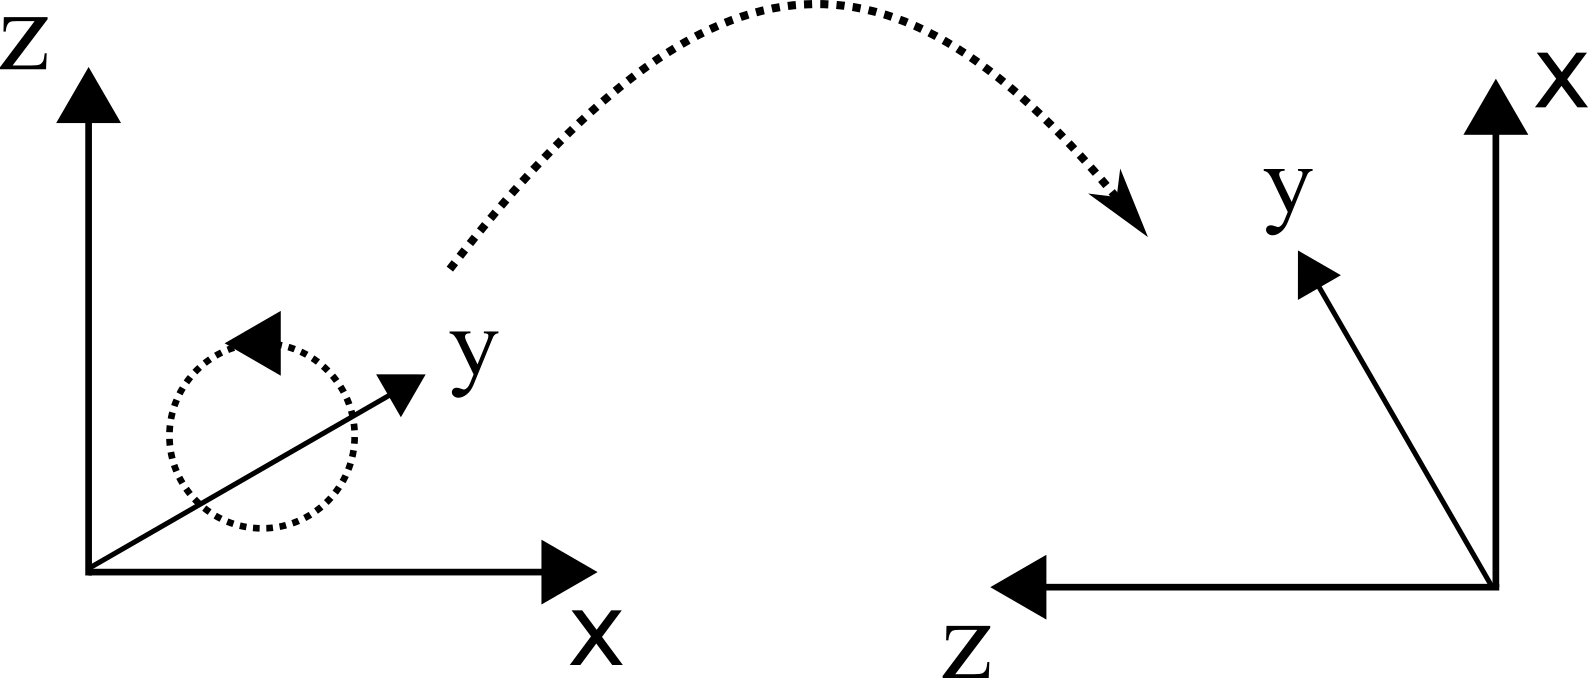
\includegraphics{./appen/rotateaxes.png}
\caption{Rotation of axes by Euler rotation $R(0\frac{\pi}{2}0)$ \label{fig:rotateaxes}.}
\end{center}
\end{figure}

For the purposes of working with the Slater-Koster parameters in 
a tightbinding Hamiltonian it remains to determine the representation of
the symmetry operation in the basis of the spherical harmonics.

The elements of the matrix representation of this symmetry operation 
can be given by $D^{l}(\Rs(0\beta0))_{m,m'}$; these are sometimes reffered to as 
the Wigner matrices. The elements of the Wigner matrix can be computed using the Euler angles
appropriate for the symmetry operation. For the example we have chosen the symmetry representation
in the basis of spherical harmonics is:
%
$\left[\begin{array}{ccccc}
0  & -1 &  0 & 0 & 0 \\
1  &  0 &  0 & 0 & 0 \\
0  &  0 & -1 & 0 & 0 \\
0  &  0 &  0 & \frac{1}{2} & \frac{1}{2}\sqrt{\frac{3}{2}} \\
0  &  0 &  0 & \frac{1}{2}\sqrt{\frac{3}{2}} & \frac{1}{2}
\end{array}\right]$
%

\section{Rotating Slater-Koster Coefficients}
The Slater-Koster coefficients are at the heart of the tight-binding method.
The Slater-Koster table plays the role for a materials scientist that a table 
of logarithms may have for a 19th century clerk.
The table is composed of the Slater-Koster coefficients 
and the energy integrals. The latter are the matrix
elements between spherical harmonics centered on two atoms and separated
by the vector $R_a$ (see Fig.\ref{SK}). 
The coefficients in that table are expressions involving combinations 
of the direction cosines connecting the two atoms.
These arise naturally from the rotation matrices required 
to reorient the vector connecting two sites so that the two
sites are oriented purely along the axis $z$.
In this frame Slater-Koster then make a further approximation
by assuming the energy integrals can be resolved in terms
of $\sigma$, $\pi$, $\delta$ bonds. This is accomplished by writing:
%
\begin{equation}
R(\alpha\beta\gamma) \bra l_{1}m'_{1}|H|l_{2}m'_{2}\ket = R(\alpha\beta\gamma)\bra l_{1}m'_{1}|H|l_{2}m'_{2}\ket' \delta_{m'_1,m'_2}
\end{equation}
%
In the Slater-Koster two center approximation the Hamiltonian matrix 
element between two states in an arbitrary position, one relative to the other is written:
%
\begin{equation}
H_{\alpha\beta}= \sum_{m_{1}'}J(l_{1}m_{1},l_{2}m_{2}m'_{1}) \bra l_{1}m_{1}'|H|l_{2}m_{1}' \ket
\end{equation}

%Sharma's J function is equivalent to the Slater-Koster coefficients and in terms of rotation
%matrices for the spherical Harmonics is written:
%\begin{equation}
%J(l_1 m_1 l_2 m_2 m'_{1}) = D^{l_1}*_{m_1',m_1}(\alpha\beta\gamma)D^{(l_2)}_{m'_1,m_2}(\alpha\beta\gamma).
%\end{equation}

Thus when the energy integrals have been determined, by computation or interpolation,  
they can be rotated by the Slater-Koster coefficients to an arbitrary position 
in a new reference frame. This allows Hamiltonians for a variety of crystals, 
BCC, FCC, HCP, diamond etc., to be easily initialized and studied in terms of a 
local geometric picture of the electron interactions in a basis of spherical harmonics. 

\section{Derivatives of Slater-Koster Parameters}
If we choose to work in spherical coordinates centered on one atom with 
the vector between our starting atom and the target atom denoted $R_{ij}$.

The correspondence between the Cartesian system and the spherical one can be given
in the usual way:
%
\begin{align}
x = r\cos\theta\sin\phi \\
y = r\sin\theta\sin\phi \\
z = r\cos\phi
\end{align}

with the inverse map:
%
\begin{align}
r=\sqrt{x^{2}+y^{2}+z^{2}} \\
\theta = \tan^{-1}(\frac{y}{x}) \\
\phi = \cos^{-1}(\frac{z}{r})
\end{align}

We will switch between $R$ and $r$ to denote the radial coordinate but
from the context it should not raise any issues. 

One quantity of interest is the derivative of the bond integral
matrix elements in the tight binding formalism which we write
as $\nabla^{ij}_{\alpha}h^{nq}_{ij}$.

The Slater-Koster parameters are given in terms of the direction
cosines of the vector connecting the two atoms $R_{ij}$ written
$l,m,n$. These direction cosines can enter the Slater-Koster expressions
linearly, as squares, or to the fourth power.

In spherical coordinates the gradient can be written:
%
\begin{equation}
\nabla =  \hat{r} \frac{\partial}{\partial r} 
          + \frac{1}{r}\hat{\phi}\frac{\partial}{\partial\phi}
          + \frac{1}{r\sin\phi}\hat{\theta}\frac{\partial}{\partial \theta}
\end{equation}

It is also useful to have the Cartesian partial derivatives written in spherical
coordinates for reference:

\begin{flalign}
\label{eq:cartpartials}
\frac{\partial}{\partial x}  =& \cos\theta\sin\phi\frac{\partial}{\partial r}
                             - \frac{\sin\theta}{r\sin\phi}\frac{\partial}{\partial \theta}
                             + \frac{\cos\theta\cos\phi}{r}\frac{\partial}{\partial \phi}\\
\frac{\partial}{\partial y}  =& \sin\theta\sin\phi\frac{\partial}{\partial r}
                             + \frac{\cos\theta}{r\sin\phi} \frac{\partial}{\partial \theta}
                             + \frac{\sin\theta\cos\phi}{r} \frac{\partial}{\partial \phi}\\
\frac{\partial}{\partial z}  =& \cos\phi\frac{\partial}{\partial r}
                             - \frac{\sin\phi}{r}\frac{\partial}{\partial\phi}
\end{flalign}

\section{Two Center Derivatives of Bond Integrals}
We will assume in what follows a scaling of the energy integrals 
as the inverse fifth power of the distance between the atoms.
The precise functional form chosen for this decay does not change
the principles of the following derivation.

We may write the integrals:
%
\begin{equation}
h^{rs}_{ij} = \frac{f_{rs}(l,m,n)}{R_{ij}^{5}}
\end{equation}
where $rs$ is the combination of spherical harmonics and $ij$ are the atom sites.
Let us look at how this energy integral varies with a perturbation of atom $i$ along $x$.
We can choose a couple different coordinate systems to take the derivative efficiently.
One way to do it is convert all the direction cosines into cartesian coordinates.

The partial derivative with respect to $\alpha = x,y,z$ are then:
%
\begin{equation}
\label{eq:derivSK}
\frac{\partial h^{rs}_{ij}}{\partial \alpha} = (\frac{-5}{R^{6}})(\frac{\partial R}{\partial \alpha})f^{rs}(l,m,n) 
                                             + \frac{1}{R^{5}}\frac{\partial f^{rs}(l,m,n)}{\partial \alpha}
\end{equation}
%
where f(l,m,n) is the Slater-Koster integral for the orbital combination $rs$.
The derivate of $R$ w.r.t to $x$ gives the direction cosine $l=x/R$ so the first contribution to the 
derivative is just the direction cosine for $x$, i.e. $l$, multiplied by 
the standard Slater-Koster term and weighted by the radial decay. 
The second term is the derivative of the Slater-Koster term with 
respect to a cartesian coordinate. This can be handled using the chain rule:
%
\begin{equation}
\frac{\partial f^{rs}(l,m,n)}{\partial x} = \frac{df^{rs}(l,m,n)}{dl}\frac{dl}{dx}
\end{equation}
%

NB the variation of the other direction cosines, $m,n$, w.r.t. $l$, and 
$l$ w.r.t. $x$: 
%
\begin{align}
\frac{dm}{dl} = \frac{-ml}{(1-l^2)} \\
\frac{dn}{dl} = \frac{-nl}{(1-l^2)} \\
\frac{dl}{dx} = \frac{(1-l^{2})}{R}
\end{align}
%
These terms contribute additional terms to the derivatives of the 
two center Slater-Koster terms. Eq.~\ref{eq:derivSK} then 
gives the first order variation of the matrix elements for
an $~R^{-5}$ dependence of the hopping integrals.

\subsubsection{Example: $h^{xy,yz}$ }
Let us take the Slater-Koster coefficient for $h^{xy,yz}$. 
We can write this overlap integral in terms of the two center bond integrals 
and the direction cosines as (after a slight rearrangement from the original table):
% 
\begin{equation}
h^{xy,yz} = \frac{ln(dd\pi-dd\delta) + lm^{2}n (3dd\sigma-4dd\pi+dd\delta)}{R^5}
\end{equation}
%

The angular part (i.e. the contribution to the derivative from the first order variation in 
the Slater-Koster coefficients w.r.t. $l$) is:

\begin{equation}
\frac{d{f^{xy,yz}(lmn)}}{dl} = (n + \frac{dn}{dl})(dd\pi-dd\delta) 
                                                  + (m^{2}n +2lmn\frac{dm}{dl}+lm^{2}\frac{dn}{dl})(3dd\sigma-4dd\pi+dd\delta)
\end{equation}

Adding the radial contribution gives the total partial derivative with respect to a cartesian coordinate:
%
\begin{equation}
\frac{\partial h^{xy,yz}_{ij}}{\partial x} =  \frac{1}{R^{6}}[-5lf^{xy,yz}(l,m,n) + (1-l^{2})\frac{df^{xy,yz}(l,m,n)}{dl}]
\end{equation}
%

   % Group Theory
%\clearemptydoublepage
\end{appendices}
\small
\bibliographystyle{cj}
\bibliography{./bibli/merged.bib}
\end{document}

